\documentclass[fyp,12pt]{socreport}

% Some generic packets.
\usepackage{color, colortbl}
\usepackage{url}
\usepackage{graphicx}
\usepackage{caption}
\usepackage{subcaption}
\usepackage{pgfplots}
\usepackage{tabularx}
\usepackage{multirow}
\usepackage{listings}
\usepackage{fullpage}
\usepackage{amsthm}
\usepackage{amssymb}
\usepackage{hyperref}
\usepackage{algorithm}
\usepackage[noend]{algpseudocode}
\usepackage[activate={true,nocompatibility},final,tracking=true,kerning=true,spacing=true,factor=1100,stretch=10,shrink=10]{microtype}
\usepackage{booktabs}
\usepackage{siunitx}



\theoremstyle{definition}
\newtheorem{defn}{Definition} \newcommand{\defnautorefname}{Definition}
\theoremstyle{plain}
\newtheorem{rul}{Rule} \newcommand{\rulautorefname}{Rule}
\newtheorem{thm}{Theorem} \newcommand{\thmautorefname}{Theorem}
\newtheorem{lemma}{Lemma} \newcommand{\lemmaautorefname}{Lemma}
\newtheorem{coroll}{Corollary} \newcommand{\corollautorefname}{Corollary}
\newcommand{\probP}{\text{I\kern-0.15em P}}
\pgfplotsset{width=10cm,compat=1.9}

% Sets the root path to look for all images.
\graphicspath{{images/}}

% Sets default options for listings.
\renewcommand\lstlistlistingname{List of Listings}
\newcommand*\lstinputpath[1]{\lstset{inputpath=#1}}
\lstinputpath{listings}
\lstset{frame=single, tabsize=2, captionpos=b}
\newcommand{\itab}[1]{\hspace{0em}\rlap{#1}}
\newcommand{\tab}[1]{\hspace{.11\textwidth}\rlap{#1}}
\newcommand{\algorithmautorefname}{Algorithm}

\usepackage{mathtools}
\DeclarePairedDelimiter{\ceil}{\lceil}{\rceil}
\DeclarePairedDelimiter{\floor}{\lfloor}{\rfloor}
\DeclarePairedDelimiter{\vbar}{\vert}{\vert}
\DeclarePairedDelimiter{\vbarbar}{\Vert}{\Vert}
\DeclarePairedDelimiter{\parenLR}{\lparen}{\rparen}
\DeclarePairedDelimiter{\brackLR}{\lbrack}{\rbrack}
\DeclarePairedDelimiter{\braceLR}{\lbrace}{\rbrace}
\DeclareMathOperator*{\argmin}{arg\,min}
\DeclareMathOperator*{\argmax}{arg\,max}

%%% Handy commands for image/figure insertion
\newcommand*{\RootPicDir}{pic}
\newcommand*{\PicDir}{\RootPicDir}
\newcommand*{\ResetPicDir}{\renewcommand*{\PicDir}{\RootPicDir}}
\newcommand*{\SetPicSubDir}[1]{\renewcommand*{\PicDir}{\RootPicDir/#1}}
\newcommand*{\Pic}[2]{\PicDir/#2.#1}

\newcommand*{\RootExpDir}{exp}
\newcommand*{\ExpDir}{\RootExpDir}
\newcommand*{\ResetExpDir}{\renewcommand*{\ExpDir}{\RootExpDir}}
\newcommand*{\SetExpSubDir}[1]{\renewcommand*{\ExpDir}{\RootExpDir/#1}}
\newcommand*{\Exp}[2]{\ExpDir/#2.#1}

\newcommand*{\BeforeCaptionVSpace}{1ex}
\newcommand*{\BeforeSubCaptionVSpace}{0.75ex}

\begin{document}
\pagenumbering{roman}

% Replace as necessary
\title{Data-driven and Physics-inspired Machine Learning: Benchmarking quantum-inspired quadratic unconstrained binary optimisation solvers}
\author{Guo Yulong}
\projyear{2023/2024}
\projnumber{H0811550}
\advisor{Assoc Prof St\'ephane Bressan}
\deliverables{
    \item \itab{Report:} \tab{1 Volume}
}
\maketitle

% Replace as necessary
\begin{abstract}
The quadratic unconstrained binary optimisation (QUBO) problem represents a cornerstone in combinatorial optimisation that encapsulates various scientific and industrial optimisation problems. However, the QUBO problem is NP-hard and is traditionally extremely difficult to solve efficiently due to the exponentially increasing search space. Our work aims to measure the performance of different quantum-inspired QUBO solvers that utilise quantum effects to search for optimal solutions. We benchmark the D-Wave Quantum Annealer, Neural Network Quantum States (NNQS), and Quantum Approximate Optimization Algorithm (QAOA) solvers with classical commercial QUBO solvers. We use a dataset with various combinatorial problems---not-all-equal 3-satisfiability, max-cut, and the Sherrington-Kirkpatrick model (SK model), and the solvers will be evaluated based on the average normalised energy and success probability. Our results show that the D-wave and NNQS solvers outperform the QAOA solver but cannot match the performance of commercial QUBO solvers. However, the D-wave solver shows promising performance compared to the GUROBI solver for some problem sizes when we match the solver runtimes. We further investigate the performance of the NNQS solver when using different architectures and training algorithms. Our results show that the NNQS with a Restricted Boltzmann Machine and a continuous training algorithm perform best across all datasets.

\begin{descriptors}
    \item \itab{10002950.10003714.10003716.10011136 Discrete optimization}
    %\item \itab{10002950.10003714.10003716.10011136 Mathematics of computing~Discrete optimization}
    \item \itab{10010405.10010432.10010441 Applied computing~Physics}
    \item \itab{10010147.10010257.10010293.10010294 Neural networks}

\end{descriptors}
\begin{keywords}
    Quadratic unconstrained binary optimisation, Ising model, Quantum annealing, Neural network quantum states, Quantum Approximate Optimization Algorithm
\end{keywords}

% Replace/Delete as necessary
\begin{implement}
    \item{Linux, GPUs, Tesla A100, Python, Tensorflow, Dimod, Qiskit}
\end{implement}

\end{abstract}

% Replace as necessary
\begin{acknowledgement}
I would like to thank my friends and family for their invaluable support during the project. I would also like to thank my project advisor, Associate Professor St\'ephane Bressan, research fellow Lu Jianlong, and past and present research group members for their invaluable guidance and support.
\end{acknowledgement}

\listoffigures % Remove if no figures
\listoftables % Remove if no tables
\tableofcontents

% Actual contents in the contents folder.
% Include additional tex files here.
\SetPicSubDir{ch-Intro}

\chapter{Introduction}
\vspace{2em}

\section{Motivation}
The quadratic unconstrained binary optimisation (QUBO) problem can represent various types of combinatorial optimisation problems and has vast applications in both operational research and industry~\cite{b1}. Most problems that involve choosing a set of binary decisions to optimise an objective function can be expressed as a QUBO problem. Examples include the max-cut problem, knapsack problem, or even problems with more complex constraints, such as the travelling salesman problem \cite{b10}. However, QUBO problems are NP-hard and are extremely hard to solve efficiently~\cite{barahona1982computational,b1}. Traditionally, QUBO-solving methods are specialised for a specific problem domain to leverage each problem domain's unique characteristics, limiting the versatility and portability of QUBO-solving methods~\cite{b5}.

The QUBO problem shares similarities with the Ising model in Physics, where the spin variables are either $-1$ or $1$, instead of the binary variables used in QUBO. The two models are equivalent, and the correspondence between the QUBO problem and the Ising model has opened the doors to solving QUBO problems with quantum computational methods~\cite{b5}. The equivalence enhances the problem domains that could be modelled as QUBO problems and allows for QUBO problems to be solved by more general quantum-inspired solving methods~\cite{b5}.

With a broad range of classical and quantum-inspired methods available to tackle QUBO problems, it is imperative to consolidate and benchmark existing QUBO-solving solvers to highlight their performance when solving different kinds of QUBO problems across a range of problem sizes.

\section{Objectives}
In the first section of the report, we aim to measure the performance of 3 quantum-inspired QUBO-solving solvers:
\begin{enumerate}
    \item Quantum Annealing
    \item Neural Network Quantum States
    \item Quantum Approximate Optimization Algorithm
\end{enumerate}
We will also use classical solvers as a baseline for comparison with quantum-inspired solvers. We will explore two classical solvers:
\begin{enumerate}
    \setcounter{enumi}{3}
    \item Fixstars Amplify QUBO Solver
    \item GUROBI Optimizer
\end{enumerate}

%QUBOs are not always effective in practice, though. In particular, they cannot directly:

%Support common real-world situations, such as continuous variables (e.g., prices, commodity flow)
%Support constraints (e.g., max/mins, price cannot exceed a certain value)
%Prove optimality (e.g., you can’t be sure you’ve identified the best solution)

For each solver, we will calculate the success rate (probability of solving optimally) and normalised energy (relative performance of candidate solution) across QUBO problems of different types and sizes. More details of the solvers and performance metrics are available in \autoref{review} and \autoref{methodology}.

In the second section of the report, we will further explore how Neural Network Quantum States can be used to simulate the quantum annealing process to solve QUBO problems. We systematically compare two neural network architectures and three different training algorithms highlighted in \autoref{nnqsresults} for Neural Network Quantum States.

The results of the study will allow us to better understand the current landscape of these quantum-inspired QUBO solvers and how they compare to state-of-the-art classical commercial solvers.
\SetPicSubDir{background}

\chapter{Background and Preliminaries}
\vspace{2em}

\section{Quadratic unconstrained binary optimization}
The quadratic unconstrained binary optimization (QUBO) problem is usually defined as
\begin{equation} 
\argmin_{x \in \{0, 1\}^n} x^\intercal Q x
\end{equation}
where $Q \in \boldsymbol{M}_{n\times n}(\mathbb{R})$ is an upper triangular square matrix with real coefficients and $x$ is a binary input vector~\cite{b1}. The matrix $Q$ characterizes the QUBO problem and can be thought of as a way of representing the QUBO problem. $x^\intercal Q x$ is also known as the objective function for the problem. Some characteristics of QUBO problems are summarised below:
\begin{itemize}
    \item The possible input space grows exponentially with the size of the problem $n$ and makes the QUBO problem NP-hard and difficult to solve efficiently.
    \item In general, the solution of a QUBO problem does not need to be unique as multiple input $x$'s can produce the same objective value.
    \item The objective function $x^\intercal Q x$ can also be expressed as $\sum_{i=1}^{n}\sum_{j=1}^{n} Q_{ij}x_{i}x_{j}$ which intuitively means that we sum up the coefficients $Q_{ij}$ where both $x_{i}$ and $x_{j}$ are $1$.
    \item The density $d$ of a QUBO problem refers to the number of non-zero elements above the main diagonal of $Q$ (quadratic terms) divided by the total number of elements above the main diagonal. 
    \item We can also express a QUBO problem as a maximization problem by using finding $\argmax_{x \in \{0, 1\}^n} -x^\intercal Q x$.
\end{itemize}

Problems that are concerned with finding the best set of binary decisions to optimize an objective function can generally be formulated as a QUBO problem~\cite{b5}. Thus, the QUBO problem model has applications in a wide range of combinatorial optimization problems such as Max-Cut~\cite{b2}, number partitioning~\cite{b3}, and machine scheduling problems~\cite{b4}. 

Once an optimization problem is expressed in a QUBO format, we can utilize general QUBO-solving methods to efficiently obtain solutions to the original problem without specializing in a particular problem domain~\cite{b1}. The following sections will describe multiple examples of QUBO problems and reformulations.

\subsection{Example QUBO problem}\label{subsection:example_qubo}
Consider the objective function \begin{equation}
f(x_1, x_2, x_3) = -8x_1 + 6x_2 + 3x_3 - 2 x_1 x_2 + 4 x_2 x_3
\end{equation} where $x_1, x_2, x_3 \in \{0, 1\}$ and we want to minimise $f$ over all possible ($x_1$, $x_2$, $x_3$) (if we wanted to maximise $f$ instead we can simply multiply all the coefficients of $f$ by $-1$). Since the variables are binary, $x_i^2 = x_i$ for all $i$, we can redefine the objective function as 

\begin{equation}
f(x) = x^\intercal Q x, \text{ where } x = \begin{bmatrix}
x_1 \\
x_2 \\
x_3 
\end{bmatrix}, \text{ }
Q = \begin{bmatrix}
-8 & -2 & 0\\
0 & 6 & 4\\
0 & 0 & 3
\end{bmatrix}
\end{equation}

The coefficients for $Q_{ii}$ are equal to the coefficient of $x_i$ in the original objective function while the coefficient for $Q_{ij}$ where $i < j$ is the coefficient of $x_{i}x_j$ while the coefficients in the lower triangular portion of $Q$ is $0$. This is a simple QUBO problem and can be solved by enumerating all the possible inputs to obtain the optimal solution of $x_1 = 1, x_2 = 0, x_3 = 0$, and $f(1,0,0) = -8$.

\subsection{Knapsack problem}
In this section, we give an example of how a combinatorial optimization problem with inequality constraints can be formalized as a QUBO problem. The knapsack problem is a classic combinatorial optimization problem where we have a knapsack with integer weight capacity $W > 0$ and $n$ items each having a weight $w_i > 0$ and profit $c_i > 0$. The problem seeks to find the optimal set of items to place in the knapsack to maximize total profit while not exceeding the knapsack weight limit. Formally, we have
\begin{align}
\max &\sum_{i=1}^n c_i x_i \label{eq:knapsack_cost}\\
\mathrm{st.} &\sum_{i=1}^n w_i x_i \leq W \label{eq:knapsack_constraint}\\
x_i &\in \{0,1\}^n \nonumber
\end{align}
The quantity \refeq{eq:knapsack_cost} refers to the total profit of the chosen items and constraint \refeq{eq:knapsack_constraint} keeps the total weight below the weight limit. To convert this optimization problem into a QUBO problem, we can include the inequality constraint in our QUBO formulation by introducing slack variables, $y_j$'s, which turn the inequality constraint into an equality constraint~\cite{b6}.
\begin{align}
\max &\sum_{i=1}^n c_i x_i \\
\mathrm{st.} &\sum_{i=1}^n w_i x_i = \sum_{j=1}^W jy_j \label{eq:knapsack_slack_weight}\\
&\sum_{j=1}^W y_j = 1 \label{eq:knapsack_slack_sum}\\
x &\in \{0,1\}^n, y \in \{0,1\}^W \nonumber
\end{align}
The slack variables $y_j$'s track the total weight of the knapsack with $y_j = 1 \Leftrightarrow$ total weight is $j$. Constraint \refeq{eq:knapsack_slack_sum} ensures that only one of $y_j$ is equal to $1$. With penalty parameters $C_1 > \sum_{i=1}^n c_i$ and $C_2 > \sum_{i=0}^n c_i$, we can formulate the following QUBO problem:
\begin{align}
    \max f(x, y) &\coloneqq \sum_{i=1}^n c_i x_i - C_1 P_w^2 - C_2 P_n^2 \\
    P_w &\coloneqq \sum_{i=1}^n w_i x_i - \sum_{j=1}^W jy_j \\
    P_n &\coloneqq 1 - \sum_{j=1}^W y_j \\
    x &\in \{0,1\}^n, y \in \{0,1\}^W \nonumber
\end{align}
Since the penalty parameters are chosen to be larger than $\sum_{i=1}^n c_i$, the optimal solution to the QUBO problem must have $P_w = P_n = 0$. Hence, ensuring that exactly one of the $y_i=1$ and the total weight is below the knapsack capacity. Since the optimal solution to the original knapsack must also have a total weight below the knapsack capacity, the value of $x$ that solves the QUBO must also solve the original knapsack problem. We can also formulate this QUBO problem in terms of $Q$ by following similar steps as \autoref{subsection:example_qubo}.

\subsection{Practical applications}
There are numerous practical scenarios where QUBO formulations can be utilized. 
\begin{itemize}
    \item~\cite{b7} uses real-world data of the location of DB Schenker shipping hubs in Europe to solve the shipment rerouting problem which aims to reduce the total distance traveled to fulfill a set of shipments.
    \item~\cite{b8} uses a QUBO formulation to solve portfolio optimization problems using real-world stock data sets of the New York Stock Exchange.
    \item~\cite{b9} formulates an image binarization method as a QUBO problem where the objective is to segment an image into its foreground and background which has further possible medical applications to improve x-ray imaging.
\end{itemize}
These practical applications of the QUBO problem motivate further exploration into different ways that QUBO problems can be solved efficiently which are explained further in \autoref{review}.

\section{The Ising Model}
The Ising model in Physics, proposed by Ernst Ising in 1925, can be thought of as a model of a magnet~\cite{isingising} and has been widely studied in Physics for its phase transition properties~\cite{cipra1987introduction}. The Ising model serves as the bridge that allows for QUBO problems to be solved with quantum-based methods~\cite{b10}. In the classical Ising model, a magnet consists of $n$ molecules that are `constrained to lie on the sites of a regular lattice'~\cite{b11}. Each molecule $i$ can be treated as a `microscopic magnet' that points along some axis and has a `spin' ($s_i$) that is either $+1$ (parallel to the axis) or $-1$ (anti-parallel to the axis). With $n$ particles, the system can then have $2^n$ states, each corresponding to a configuration of the individual molecule spins.


\subsection{Ising Hamiltonian}
In quantum mechanics, the Hamiltonian of a system $\Hat{H}$, is a linear operator that represents the total energy of a system and is a key component that governs the evolution of the system~\cite{GriffithsSchroeter2018}. \hyperref[sdd_1]{Section \ref{wavefunction}} discusses the Hamiltonian and general quantum mechanics in greater detail. For this study, we can treat the Hamiltonian as a function of the quantum system that maps a quantum state to an energy level. The possible energy levels of the system are exactly the eigenvalues of its Hamiltonian and the corresponding eigenvectors are the possible states that are mapped to the certain energy level~\cite{b21}. 

In the Ising model with $n$ particles, the Hamiltonian has two components --- the external field term (characterized by $\mathbf{h} = (h_1, h_2, ..., h_n) \in \mathbb{R}^n$) and the interaction term between molecules (characterized by a strictly upper triangular matrix $\mathbf{J} \in \boldsymbol{M}_{n\times n}(\mathbb{R})$)~\cite{b10}. We can express the Hamiltonian as a function of the $n$ spins from each particle:
\begin{equation}
    \Hat{H}(s) = \Hat{H}(s_1, s_2, ... , s_n) = -\sum_{1\leq i < j \leq N} J_{ij}s_i s_j - \sum_{i=1}^N h_i s_i
\end{equation}
We can view $\mathbf{h}$ as the interaction of each particle with an external magnetic field and $\mathbf{J}$ as the coupling between pairs of spins. A positive $J_{ij}$ term means that the energy is low when spins $s_i$ and $s_j$ are aligned while a negative $J_{ij}$ term means that the energy is low when the spins are anti-aligned. A large value of $h_i$ means that the spin $s_i$ tends to be aligned or anti-aligned with an external magnetic field in the ground state.
The Ising model was initially proposed to study phase transitions of the system at certain critical temperatures by solving for the ground state of the system at different temperatures~\cite{isingising}. To find the ground state---the state of spins that minimizes the total system energy of the Ising model---we have to solve for $ \argmin \Hat{H}(s) $ for $ s \in \{ 0, 1 \}^N $. This is equivalent to a corresponding QUBO problem up to a change in the variable domain (from spins to binary variables). The equivalence of the QUBO problem and the Ising model is one of the most significant applications of QUBO~\cite{b5}. We will show in the following subsections how we can convert a QUBO problem into an Ising model and vice versa.

\subsection{Converting QUBO to Ising}
Given a QUBO problem with QUBO matrix $Q$, we can use the conversion, $x_i = \frac{s_i + 1}{2}, s_i \in \{-1, 1\}$ to change the spin variables into binary variables. The objective function $f(x)$ of the QUBO problem can be expressed as
\begin{align}
    f(x) &= f(x_1, ..., x_n) \nonumber\\
    &= \sum_{1\leq i < j \leq n} Q_{ij}(x_i x_j) + \sum_{i=1}^N Q_{ii} x_i \nonumber \\
    &= \sum_{1\leq i < j \leq n} \frac{1}{4} Q_{ij}(s_i + 1)(s_j + 1) + \sum_{i=1}^N \frac{1}{2} Q_{ii} (s_i + 1) \nonumber
\end{align}
If we group the constant terms into $k$ and let $a_i = \sum_{1\leq j \leq N, j \neq i} \frac{1}{4}Q_{\min(i,j)\max(i,j)} + \frac{1}{2}Q_{ii}$, we can express the objective function as:
\begin{align}
    f(x) = \sum_{1\leq i < j \leq n} \frac{1}{4} Q_{ij}s_i s_j + \sum_{i=1}^N a_i s_i + k \nonumber
\end{align}
Removing the constant $k$ which is irrelevant for optimization, we can reformulate the QUBO problem as an Ising model with $h_i = -a_i$ and $J_{ij} = -\frac{1}{4}Q_{ij}$ for $i \neq j$. Finding the ground state for the Ising model is the same problem as finding $\argmin_{x \in \{0, 1\}^n} x^\intercal Q x$, and the solution to the ground state of the Ising model can be mapped to a solution for QUBO problem using $x_i = \frac{s_i + 1}{2}$. However, note that the optimal objective function value may be different due to the constant $k$.

\subsection{Converting Ising to QUBO}
Given the Hamiltonian of an Ising problem, we use the conversion $s_i = 2x_i - 1, x_i \in \{0, 1\}$ to change the spin variables into binary variables:
\begin{align}
    \Hat{H}(s) &= -\sum_{1\leq i < j \leq n} J_{ij}s_i s_j - \sum_{i=1}^N h_i s_i \nonumber\\
    &= -\sum_{1\leq i < j \leq n} J_{ij}(2x_i - 1) (2x_j - 1) - \sum_{i=1}^N h_i (2x_i - 1) \nonumber\\
    &= -\sum_{1\leq i < j \leq n} J_{ij}(4x_i x_j - 2x_i - 2x_j + 1) - \sum_{i=1}^N (2h_i x_i - h_i) \nonumber
\end{align}
If we group the constant terms into $k$ and let $a_i = 2h_i + \sum_{1\leq j \leq N, j \neq i} 2J_{\min(i,j)\max(i,j)}$, we can express the Hamiltonian as:
\begin{align}
    \Hat{H}(s) &= -\sum_{1\leq i < j \leq n} 4J_{ij}x_i x_j - \sum_{i=0}^N a_{i}x_i + k \nonumber
\end{align}
Removing the constant $k$ which is irrelevant for optimization, we can reformulate the Ising model Hamiltonian as a QUBO matrix $Q$ such that $Q_{ii} = -a_i$ and $Q_{ij} = -4J_{ij}$ for $i < j$. Finding $\argmin_{x \in \{0, 1\}^n} x^\intercal Q x$ is now the same problem as finding the ground state for the original Ising model and the solution to the ground state of the Ising model can be mapped to a solution for QUBO problem using $s_i = 2x_i - 1$. However, note that the optimal objective function value may be different due to the constant $k$.

\section{Solving for the ground state of the Ising model}
In one and two-dimensional Ising models, where each particle can only interact with two or four direct neighbors, the ground state can be solved through exact methods such as calculating the partition function~\cite{onsager} or using the transfer matrix method~\cite{kramerising}. However, when solving for the ground state of higher dimension Ising models, which are those that we are interested in, exact methods are computationally intractable for large systems since the computational resources scale exponentially with the number of spins~\cite{barahona1982computational}. However, there are ways to approximate the ground state such as with the Metropolis-Hastings algorithm \cite{metropolissampling} which can be used to increase the probability of finding the ground state of the system. More details for methods of solving Ising models that have higher dimensions can be found in \autoref{review}.

\section{Wave functions, Observables and Ansatzes}\label{wavefunction}
Quantum physics is built around wave functions and operators \cite{GriffithsSchroeter2018}. Wave functions represent the state of the system and live in a Hilbert space, which is the set of all square-integrable functions:
\begin{equation*}
    f(x) \text{ such that } \int_{-\infty}^\infty |f(x)|^2 \; dx < \infty
\end{equation*}
This is generally an infinite dimensional complex vector space and allows for the wave function, denoted as $\Psi$, to be normalized so that $\int_{-\infty}^\infty |\Psi|^2 \; dx = 1$. Under the statistical interpretation of quantum mechanics, $|\Psi(x)|^2$ would also represent the probability of a system being in state $x$ once it is measured. This also means that a wave function can exist as a superposition of states. For this project, we will adopt the statistical interpretation and view the wave function as simply a probability distribution over all possible state configurations.

Quantum operators represent the observables---measurable quantities of the system such as position, momentum, or energy. Quantum operators are hermitian linear operators that act on a wave function to map states to real values. The eigenvalues of the operator have to be real as they correspond to one of the possible measured values of the represented quantity. When an operator acts on a wavefunction that exists as a superposition of multiple states, it returns an expected value of the observable instead. The Hamiltonian, which is the energy operator, is the main operator used in this study and the set of eigenvalues of the Hamiltonian are all the possible energies that the system could have. 

For an Ising model, the wavefunction encodes the probabilities of each configuration of spins and the Hamiltonian maps each wavefunction to an energy level. If a wave function only has one possible configuration, the Hamiltonian will return the eigenvalue that matches the energy level of the state. If the wave function is in a superposition of states, the Hamiltonian will return a linear combination of the eigenvalues instead.

An Ansatz is an educated guess for the solution to a problem and often involves a reduction in the complexity or size of the problem \cite{qaoareview}. When solving for the ground state of a wave function with variational methods, an Ansatz is used to represent a subspace of the infinite-dimensional Hilbert space that the wave function lives in. It is important to ensure that the wave function is general enough to closely approximate the space of all solutions yet is specific enough to be computed.
\chapter{Related Work}
\label{review}
\vspace{2em}

\section{Methods for solving QUBO problems}
There are many possible methods for solving QUBO and Ising problems which can be broadly categorized as Classical, Quantum-based, and Hybrid.

\subsection{Classical}
A typical classical approach to solving QUBO problems is by exact diagonalization of the corresponding Ising Hamiltonian \cite{b25}. Exact diagonalization solves for all the eigenvalues and eigenvectors by diagonalizing the Hamiltonian matrix \cite{b25}. This is also known as the eigendecomposition of a matrix and is possible for all real symmetric matrices \cite{b27}. However, the runtime of exact diagonalization scales exponentially with input problem size and becomes computationally infeasible once the matrix grows large \cite{b25}. Since we are only interested in finding the smallest eigenvalue and the corresponding eigenvector, we can use iterative methods such as the Lanczos algorithm or the implicitly restarted Arnoldi method to find the smallest eigenvalue \cite{b28,b29}. However, such methods often run into stability issues.

Other classical methods for efficiently solving QUBO problems rely on "heuristics and approximation algorithms" as exact methods have an exponential worst-case runtime \cite{b12}. For example, variants of Tabu search---a local search algorithm that allows for moves that are not improvements and discourages visiting already visited states---are highly competitive heuristic algorithms to find good solutions to QUBO problems\cite{b2,b30}.

Dunning et al.\cite{b12} conducted a systematic review and evaluation of published heuristics for QUBO problems and provided an open-source problem repository MQLib for further research. In addition, the solver by Dunning et al.\cite{b12} also provides a machine-learning model that predicts the best-performing set of heuristics for a given problem input.

\subsection{Quantum-based}
Quantum-based methods for solving QUBO problems include quantum annealing and neural network quantum states.

\subsubsection{Quantum Annealing}
Quantum annealing-based methods can solve for the ground state configuration of Ising models by utilizing the \textit{adiabatic theorem}\cite{b14}. The \textit{adiabatic theorem} states that "a quantum system in its ground state will remain in the ground state, provided the Hamiltonian governing the dynamics changes sufficiently slowly" \cite{b14,b15}.

Quantum annealers first prepare a system in the ground state with a simple initial Hamiltonian $H_0$, then slowly manipulate the system Hamiltonian to a more complex form $H_c$ \cite{b10}. The Hamiltonian at any point $H(s)$, where $s \in [0,1]$ is the normalized anneal fraction, can be written as

\begin{equation}
    \label{eqn:annealinghamiltonian}
    H(s) = A(s)H_0 + B(s)H_c
\end{equation}

Where $A(s)$ and $B(S)$ are decreasing and increasing functions respectively and are determined by the quantum annealing controls. If the transition time is sufficiently large, and $H_0$ and $H_c$ do not commute, the adiabatic theorem ensures that the system will remain in the ground state which can then be measured to yield the desired ground state configuration \cite{b14}.

Quantum annealing has been extensively studied and applied in multiple fields such as Scheduling Problems \cite{b17}, Portfolio Optimization \cite{b18} and Quantum simulations \cite{b19}. Even though it is debated whether Quantum Annealing will be superior to classical methods \cite{b10} and there are significant roadblocks in scaling hardware capabilities \cite{b14}, there is hope that these challenges will be solved in the near future with the rapid progress made in quantum computing research.

\subsubsection{Neural-Network Quantum States}
Carleo and Troyer \cite{b20} introduced another quantum-based method for modeling the wave function of a given Ising Hamiltonian known as \textit{neural-network quantum states} (NNQS). The wave function can be viewed as a complex probability distribution over all the possible state configurations and the NNQS method approximates the wave function of a system as an artificial neural network \cite{b25}. 

The original NNQS architecture utilized a Restricted Boltzmann Machine (RBM) to represent the wave function of an arbitrary quantum system \cite{b20}. The RBM is an energy-based machine learning model that has two layers of nodes, a visible layer $\boldsymbol{s}$, and a hidden layer $\boldsymbol{h}$, where each visible node $s_i$ represents the spin of a particle in the Ising model \cite{b20}. Each visible node $s_i$ is connected to every hidden node $h_j$ with a certain weight $W_{ij}$ but there are no connections within the visible or hidden layer \cite{b20}. The representation of the wave function by the RBM can then be expressed as

\begin{equation}
    \Psi(\boldsymbol{s}, \boldsymbol{\theta}_{rbm}) = \sum_{h} e^{\sum_i a_s s_i + \sum_j b_j h_j + \sum_{i,j}W_i s_i h_j} 
\end{equation}

where  $\boldsymbol{\theta}_{rbm} = \{\boldsymbol{a}, \boldsymbol{b}, \boldsymbol{W}\}$ are the biases and weights of the RBM \cite{b20}. The RBM is trained in an unsupervised manner. The weights $W$ are usually updated by performing Gibbs sampling, calculating the average energy of sampled configurations, and using gradient-based optimization algorithms \cite{b25}.

Other neural network architectures such as the Multilayer Perceptron (MLP) can also be used for NNQS. An MLP model consists of an input layer $\boldsymbol{x}$, one or more hidden layers, and an output layer. Each layer is fully connected to the next layer with certain weights and each node has an activation function $\sigma$ such as the sigmoid or ReLU. Each input node $x_i$ represents the spin of a particle in the Ising model and the output nodes represent the output from the wave function. If we assume that the wave function is real and positive, then only one output node is needed to represent the real part of the wave function. \cite{b20}. With one hidden layer, the MLP representation of the wave function can be expressed as

\begin{equation}
    \Psi(\boldsymbol{x}, \boldsymbol{\theta}_{mlp}) = 
    \sigma_{out} \left(
    \boldsymbol{W}_{out}
    \sigma_{hidden} \left( \boldsymbol{W}_{hidden}\boldsymbol{x} + \boldsymbol{b}_{input} \right) + \boldsymbol{b}_{hidden} \right)
\end{equation}

where  $\boldsymbol{\theta}_{mlp} = \{\boldsymbol{W}_{hidden}, \boldsymbol{b}_{input}, \boldsymbol{W}_{out}, \boldsymbol{b}_{hidden}\}$ are the weights and bias of the MLP \cite{b20}. The MLP is trained in an unsupervised manner, similar to the RBM, except that a more general sampling method, the Metropolis algorithm, has to be used \cite{b25}.

\subsection{Hybrid quantum-classical}
A third class of QUBO solving methods are hybrid quantum-classical methods which are designed to make use of current limited quantum computing resources by integrating them with classic methods to solve combinatorial optimization problems \cite{b32}. One such algorithm is the Quantum Approximate Optimization Algorithm (QAOA) which is used to find approximate solutions to general combinatorial optimization problems \cite{b23}. Similar to NNQS, QAOA aims to find an approximation of the ground state of an input Hamiltonian using gate-based quantum circuits and $2p$ parameters which are optimized with a classical computer \cite{b34}. With a problem of size $N$. the algorithm first prepares a quantum state $| + \rangle^{\otimes N}$ in uniform superposition by applying the Hadamard gate to each of the $n$ inputs \cite{b34}. The trial wave function is then constructed by

\begin{equation}
    \Psi(\boldsymbol{\gamma}, \boldsymbol{\beta}) = U_B(\beta_p) U_C(\gamma_p)...U_B(\beta_1) U_C(\gamma_1) | + \rangle^{\otimes N}
\end{equation}
\begin{align*}
    U_C(\gamma) &= e^{-i\gamma H_c} \\
    U_B(\beta) &= e^{-i\beta H_0}
\end{align*}

$U_c$ and $U_B$ are operators that evolve the state with the Hamiltonian $H_c$ (problem Hamiltonian) and $H_0$ (an easy-to-implement Hamiltonian) for times $\boldsymbol{\gamma}$ and $\boldsymbol{\beta}$ and the parameter $p$ determines the number of independent parameters of the final state \cite{b34}. The state is then measured and $\boldsymbol{\gamma}$ and $\boldsymbol{\beta}$ are chosen to minimize the average energy of the sample measurements. With the optimal parameters, the final solution can then be determined by repeatedly sampling from the trial wave function and using the state that occurs most frequently during measurements.

In contrast to quantum annealing which can only be run on specialized quantum annealing devices, QAOA can be implemented on a general gate-based quantum computer \cite{b22}. 

\section{Related benchmarking work}
Willsch et al. \cite{b34} evaluated the performance of the QAOA algorithm and the D-Wave quantum annealer using instances of MaxCut and 2-satisfiability problems with up to 18 variables. The performance of the QAOA algorithm is inconsistent and underperforms quantum annealing in their problem set \cite{b34}. 

Similarly, Pelofske et al. \cite{b35} compared the performance of QAOA and quantum annealing on Ising models with cubic interaction terms and also found that quantum annealing had superior performance over QAOA. 

Benchmarking work of NNQS against other quantum-based QUBO solving methods is unexplored.

\SetPicSubDir{ch-methodology}
\SetExpSubDir{ch-methodology}

\chapter{Methodology}
\label{methodology}
This chapter explains the methodology employed in our study, which includes the solvers, datasets, and evaluation metrics.

\section{Solvers}
We will employ five QUBO-solving-methods:
\begin{enumerate}
    \item D-Wave Quantum Annealing
    \item Neural Network Quantum States (NNQS)
    \item Quantum Approximate Optimization Algorithm (QAOA)
    \item GUROBI Optimizer
    \item Fixstars Amplify QUBO Solver
\end{enumerate}
The following sections will provide more information on the solvers used for each method.

\subsection{D-Wave Quantum Annealing}
We will use quantum annealers from D-wave Systems as the solver for Quantum Annealing. D-Wave Systems, a Canadian-based company, currently produces the most popular commercially available quantum annealing hardware and uses superconducting qubits to represent binary variables in their annealers \cite{b14}.  Given a target QUBO problem to solve, the process for using a D-Wave Systems Quantum Processing Unit (QPU) is as follows:

\begin{enumerate}
    \item \textbf{Problem Definition} QUBO problem is first converted to its corresponding Ising model Hamiltonian on the local device.
    \item \textbf{Minor Embedding} As the Quantum Processing Unit (QPU) used by D-Wave is not fully connected as shown in \autoref{pegasustopology}, a single variable in the Ising model may need to be represented by multiple qubits called a \textit{chain} which are forced to return the same value with large interaction terms \cite{b16}. This will be done with an embedder provided by the D-wave library.
    \item \textbf{Programming} The parameters of the annealing process are set, which consists of the bias for each qubit (represents magnetic field acting on each qubit) and coupler strength (represents variable interaction).
    \item \textbf{Initialization} The QPU is initialized in the ground state of an easy-to-implement initial Hamiltonian. The qubits are prepared to be in a superposition of all possible states.
    \item \textbf{Annealing} The system evolves with a time-varying Hamiltonian.
    \item \textbf{Readout of solution} The spin values of the qubits are measured and stored as a possible solution.
    \item \textbf{Resample} As the finite-time quantum annealing process does not guarantee that the system ends up in the ground state, we repeat the sampling to obtain many possible solutions that are likely to be the ground state of the initial Hamiltonian.
\end{enumerate}
\begin{figure}[h!]
    \centering
    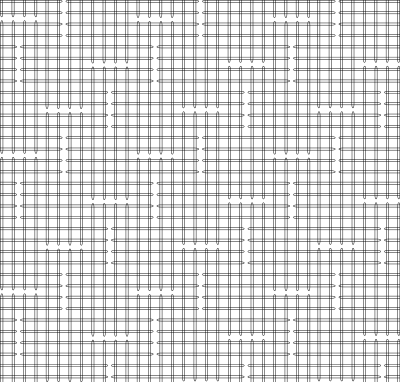
\includegraphics[width=0.5\linewidth]{images/pegasus_topology.png}
    \caption[A view of the D-Wave pegasus topology---each line represents a qubit and intersections represent available couplers]{A view of the D-Wave pegasus topology where each line represents a qubit and intersections represent available couplers~\protect\cite{dwaveadvantage}}
    \label{pegasustopology}
\end{figure}
The experiments will be conducted with the D-Wave Advantage 4.1 QPU with up to 5640 qubits and 40484 couplers \cite{dwaveadvantage}. The QPU operates at a temperature of approximately $12$mK and is built with "a network of tunably coupled rf superconducting quantum–interference device (rf-SQUID) qubits" arranged with the Pegasus graph topology that allows for up to 15 couplers per qubit, shown in \autoref{pegasustopology}. The system Hamiltonian as a function of $s$, the normalized anneal fraction, is:
\begin{equation}
    \label{eqn:dwavehamiltonian}
    H(s) = -\frac{A(s)}{2}\left(\sum_{i} \Hat{\sigma}_x^{(i)}\right) + \frac{B(s)}{2}\left(\sum_{i}h_i \Hat{\sigma}_z^{(i)}\ + \sum_{i > j}J_{i,j} \Hat{\sigma}_z^{(i)}\Hat{\sigma}_z^{j)}\right)
\end{equation}
where functions $A(s)$ and $B(s)$ used in the Advantage 4.1 QPU are shown in \autoref{dwaveannealing} with $A(s) >> B(s)$ when $s=0$ and $B(s) >> A(s)$ when $s=1$ and have an energy scale of around $10^{-24} J$.
\begin{figure}[h!]
    \centering
    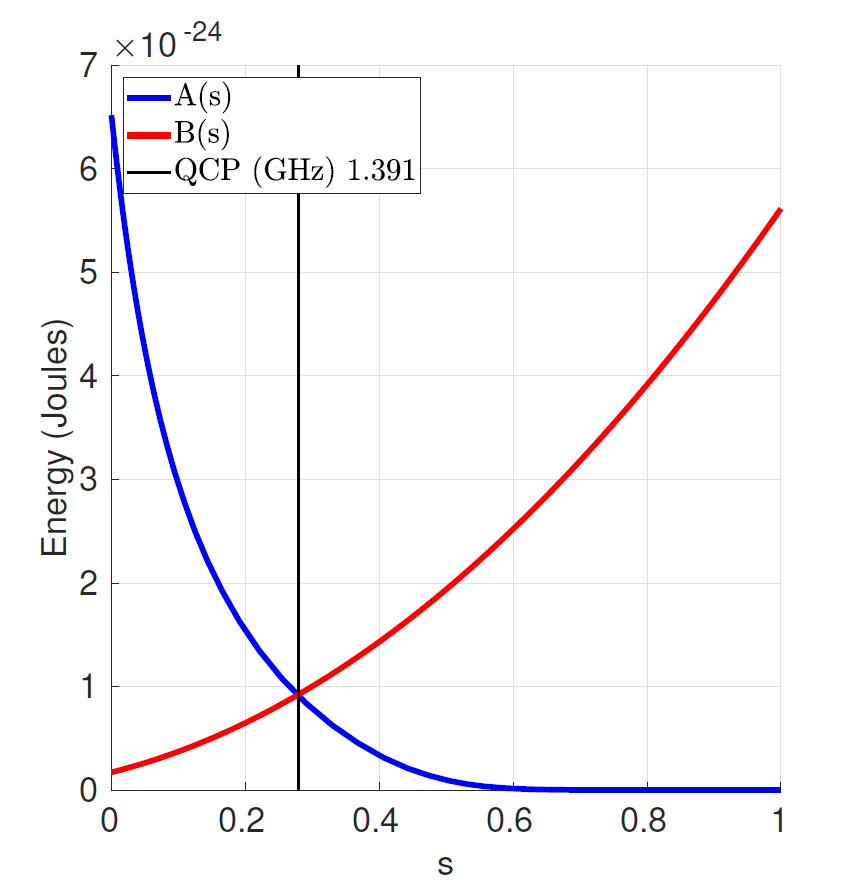
\includegraphics[width=0.6\linewidth]{images/dwave_annealing.png}
    \caption[Annealing functions $A(s)$ and $B(s)$ as a function of the normalized anneal fraction $s$]{Annealing functions $A(s)$ and $B(s)$ as a function of the normalized anneal fraction $s$~\protect\cite{dwaveadvantage}}
    \label{dwaveannealing}
\end{figure}
We will use the default annealing time of $20\mu s$ with $1000$ repeated samplings (number of reads). The candidate solution will be taken as the best solution among the $1000$ sampled configurations.


\subsection{Neural-Network Quantum States}
We will adopt the Python library MAPALUS for implementing the Neural-Network Quantum States \cite{b25}. MAPALUS uses the Tensorflow library and enables parallel execution on general-purpose graphics processing units (GPUs) for quicker sampling. In this section, we will use the Restricted Boltzmann Machine (with $5n$ hidden nodes and the sigmoid activation function) as the underlying architecture for the NNQS. 

To solve a given input QUBO problem, the NNQS will be used to simulate a quantum annealing process with a time-dependent Hamiltonian that follows \autoref{eqn:annealinghamiltonian}. Since the equations for $A(s)$ and $B(s)$ are not available, we employ a curve-fitting process to obtain analytical functions for use in the NNQS. The fitted functions used are $A(s) = 1.11e^{-7.06s} + -0.00569$ and $B(s)= 0.680s^2 + 0.288s + 0.0305$, details on the curve fitting process are available in \autoref{appendix:curvefitting}.

\begin{algorithm}
    \begin{algorithmic}
    \Require Problem Hamiltonian $\hat{H}_c$
    \Ensure Trained NNQS
    \State Initialize NNQS with random weights;
    \For {$s \in [0.1, 1.0]$ step $0.1$}
    \State Set $H(s) \leftarrow A(s)\hat{H}_0 + B(s)\hat{H}_c$;
    \State Train NNQS on $H(s)$ until convergence or until epoch limit of $100$ is reached;
    \EndFor
    \end{algorithmic}
    \caption{NNQS Progressive Training}
    \label{alg:progressive}
\end{algorithm}

The NNQS will be trained with a progressive training schedule that mimics the quantum annealing process and follows \autoref{alg:progressive}. $\hat{H}_c$ is the problem Hamiltonian and $\hat{H}_0$ is a Hamiltonian with linear biases as $1$ and no quadratic terms. The normalized anneal fraction $s$ is increased in small steps while the NNQS is trained until convergence or until the epoch limit. This ensures that the NNQS remains in the ground state throughout the training and that the problem Hamiltonian changes relatively slowly. 

The parameters of the NNQS, $\mathbf{\theta}$ are updated with a Variational Monte Carlo approach in order to minimize the energy expectation value. The general training algorithm is described as follows:
\begin{enumerate}
    \item Initialize the NNQS parameters $\mathbf{\theta}$ randomly.
    \item Sample a set of $m$ configurations $\mathbf{s}$ from the probability distribution defined by the NNQS, $\probP(s) = |\Psi(s;\theta)|^2$, with a Markov Chain Monte Carlo technique such as Gibbs sampling or the Metropolis-Hastings algorithms \autoref{samplingmethods}.
    \item Calculate the energy expectation value by taking the mean of the  energies of the sampled configurations with the Hamiltonian, which will form an unbiased estimate of the true energy expectation value.
    \item Compute the gradients of the energy expectation value with respect to the NNQS parameters using backpropagation.
    \item Update the parameters with gradient-based optimizers such as Root Mean Squared Propagation (RMSprop) \cite{rmsprop}.
    \item Repeat steps 2-5 for some iterations or until convergence is reached.
\end{enumerate}
The appendix in \cite{b20} describes the NNQS training algorithm in full. Each training process runs for at most $1000$ epochs and the model weights are updated with the RMSprop optimizer with a learning rate of $0.001$. The candidate solution will be taken as the best solution among the final $1000$ sampled configurations. All NNQS experiments were run on a 32 Core AMD 7543P Processor and an NVIDIA A100 40GB GPU with 500GB of RAM.

\subsection{Quantum Approximate Optimization Algorithm}
We will employ the implementation of QAOA in Qiskit with $p=1$ using a backend hosted on the IBM Quantum Platform (IBMQ) \cite{b24}. Even though IBMQ allows for access to quantum computers with up to 127 qubits, it is highly limited with long wait times ($>5$ hours for each problem) for a benchmarking experiment. Instead, we will be utilizing the IBMQ simulator, which is capable of handling quantum circuits with up to 32 qubits. With an input Hamiltonian $\Hat{H}_c$, we will use the default mixing Hamiltonian of $\Hat{H}_0 = \sum_{i}\Hat{\sigma}_x^{(i)}$ and a set of Hadamard gates applied to all qubits as the initial state. The Qiskit transpiler is used to optimize the decomposition of the operators into their individual parametrized quantum gates as shown in \autoref{qiskitcircuit} \cite{qiskittranspiler}.

\begin{figure}[h!]
    \centering
    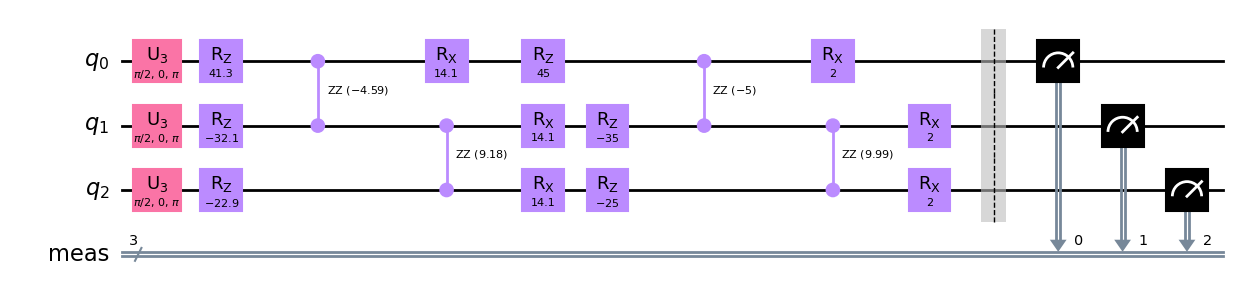
\includegraphics[width=1\linewidth]{images/qiskit_circuit.png}
    \caption{Circuit diagram with the Hadamard gates, problem Hamiltonian operator, and mixing Hamiltonian operator and  (left to right)}
    \label{qiskitcircuit}
\end{figure}

The parameters of QAOA, $(\boldsymbol{\gamma}, \boldsymbol{\beta})$ are updated to minimize the energy expectation value. The general training algorithm is described as follows:
\begin{enumerate}
    \item Initialise the circuit in the initial state $| + \rangle^{\otimes n}$ with each qubit is in a superposition state. and random initial $\gamma, \beta$. 
    \item Construct the operators $U_C(\gamma), U_B(\beta)$ with $\gamma, \beta$.
    \item Calculate the energy expectation value by taking the mean of the  energies of sampled configurations by repeatedly measuring the final states of the qubits.
    \item Use a classical derivative-free optimizer such as Constrained Optimization by Linear Approximation (COBYLA) to optimize the parameters $\gamma, \beta$ to mimimize the energy expectation value.
    \item Repeat steps 2-4 for some iterations or until convergence is reached.
\end{enumerate}
The experiments were run on the IBMQ cloud with the ibmq\_qasm\_simulator, a general-purpose simulator for simulating quantum circuits, and the COBYLA optimizer for updating the circuit parameters. We will assume an ideal circuit without a quantum noise model for measuring the optimal performance of the QAOA algorithm. We will repeatedly sample the final circuit with optimized parameters for $1000$ times and the candidate solution will be taken as the best solution among the sampled configurations.


\subsection{GUROBI Optimizer}
The GUROBI optimizer is used as a state-of-the-art classical commercial solver which is free for academic use \cite{b26}. As the GUROBI optimizer supports QUBO problems, we construct the QUBO matrix directly using the Gurobi Python library and run the optimizer locally for $10$ minutes for each input problem. If the optimizer finishes before the cutoff, the candidate solution is guaranteed to be the optimal configuration, otherwise, we would use the best solution found within the cutoff time as a candidate solution. All experiments were run on a 32 Core AMD 7543P Processor and an NVIDIA A100 40GB GPU with 500GB of RAM using Gurobi Optimizer version 10.0.3.

%All GUROBI experiments used the Gurobi Optimizer version 9.0.1 and were run on a local machine with an 8-core Apple M1 chip at 3.2GHz with 16GB of RAM.

\subsection{Fixstars Amplify QUBO Solver}
The Fixstar Amplify QUBO solver is a commercial simulated annealing-based QUBO solver that has limited free access \cite{b12}. As the Fixstar solver supports QUBO problems, we submit the QUBO matrix directly using the Fixstar API and run the solver with the highest allowed time limit which is $100$ seconds for each input problem. The solver is implemented on GPUs and is run on Fixstar remote servers which are accessed with an API token.

\section{Benchmark datasets}
We use 3 randomly generated problem sets to benchmark our QUBO solvers. These problems were chosen as they are commonly used to represent NP-hard problems to measure the performance of QUBO solvers and are relatively straightforward to encode into QUBO form. They are the not-all-equal 3-satisfiability (NAE3SAT), max-cut, and the Sherrington-Kirkpatrick (SK) model. The NAE3SAT and max-cut problem sets are macro benchmarks (application-based) to represent practical combinatorial optimization problems while the SK model problem set is a microbenchmark that is designed to test the performance of the solvers. Each problem set comprises problems of 13 sizes, ranging from $10$ to $300$\footnote{$n \in [10,15,20,25,30,35,50,75,100,150,200,250,300]$}. $20$ different random problems are generated\footnote{random seed is chosen to be from $0-19$} for each problem size $n$ for a total of $260$ problems per problem set. Each problem is also first formulated in either the QUBO or Ising form and conversion between them follows \autoref{qubotoising} and \autoref{isingtoqubo}.

\subsection*{Not-all-equal 3-satisfiability (NAE3SAT)}
The NAE3SAT problem is a variant of the boolean satisfiability problem where each problem instance consists of $n$ boolean variables $(x_1, x_2, ..., x_n)$ and $m$ clauses that each combine three literals which can be a variable or its negation. The objective is to find an assignment of boolean values such that the three values in each clause are not all the same, i.e., each clause has at least one true and one false value. The ratio of clauses to variables $\rho = \frac{m}{n}$ is a problem parameter and NAE3SAT problems are known to transition from being satisfiable to unsatisfiable at around $\rho = 2.1$ \cite{nae3sattransition}. We generate random NAE3SAT problems with $\rho = 2.1$ using the random\_nae3sat generator from the dimod D-wave Python library which "randomly samples clauses from the space of 3-variable clauses with replacement" \cite{dimodrandomnae3sat}. 

To convert a NAE3SAT problem into an Ising problem, we represent each boolean variable as a spin variable and turn each clause into a Hamiltonian term. For example, for the clause $(x_1, x_2, \neg x_3)$, we use the Hamiltonian term $H(s_1, s_2, s_3) = s_1 \cdot s_2 + s_2 \cdot (-s_3) + s_1 \cdot (-s_3)$ which has a value of $3$ when $x_1=x_2=\neg x_3$ and $-1$ otherwise. The final Hamiltonian $\Hat{H}_c$ is simply a sum of the individual Hamiltonian terms for each clause.

\subsection*{Max-cut}
The max-cut problem aims to find a partition of the vertices of a graph $G = (V, E)$ into $V_0, V_1$ with $V = V_0 \cup V_1$ and $V_0 \cap V_1 = \emptyset$, such that the number of edges crossing $V_0$ and $V_1$ is maximized. We will use the Erdos-Renyi model to generate random graphs with $n$ vertices and a probability $p=0.25$ to include each edge.

To convert a max-cut problem into a QUBO problem, we represent the assignment of each vertex as a binary variable ($x_v = i$ if $x \in V_i$) and use the objective function $f(\mathbf{x}) = \sum_{e = (u, v) \in E} -x_u - x_v + 2x_u x_v$, where each term has a value of $-1$ when $x_u  \neq x_v$ and $0$ otherwise. If a problem has a max-cut value of $C$, the objective function would have a minimum value of $-C$. 

\subsection*{Sherrington-Kirkpatrick (SK) model}
The Sherrington Kirkpatrick (SK) model is an Ising problem with a random Hamiltonian of the form $\hat{H}_c = \frac{1}{\sqrt{n}} \sum_{1 \leq i < j \leq n} J_{ij}s_i s_j$
where $J_{ij} \sim \mathcal{N}(0,1)$ are independent standard Gaussian variables. The energy landscape of the SK model is complex and has exponentially many local minima with a unique global minimum separated by high energy barriers \cite{skmodel}. This many-valley structure implies that it is extremely difficult to find the exact solution of the model. We generate random Gaussian variables with a random normal generator from the NumPy Python library.

%Parisi [6] provides a formula (for proof, see [7]) that, when numerically evaluated [8, 9, 1], shows for typical instances,
%\begin{equation*}
%    \lim_{n\rightarrow \infty} \argmin \frac{E}{n} = -0.763166...
%\end{equation*}
%(get from this paper https://quantum-journal.org/papers/q-2022-07-07-759/pdf/)

%\subsection*{Quantum Critical Points}
%get rid of linear term
%J terms are 1
%Ising model has no linear term
%QCP is A(s)/2 = +-B(s)/2 * J magnitude is the same.
%harder for Dwave to solve, jump to excited state
%finite infinite approximating

%We plan to use a subset of the 3296 QUBO problems provided by MQLib as our benchmark dataset. These problems are publicly accessible and contain both "real-world problem instances" and randomly generated problems \cite{b12}. The dataset also contains problems of various sizes and densities. The exact benchmark dataset will be determined after further testing to determine the input limits of each solver. Each QUBO problem will first be converted into an Ising model problem and then passed to each of the solvers.

\section{Performance evaluation}
To evaluate the performance of each solver we will use two performance metrics:
\begin{enumerate}
    \item The probability of finding the best solution. The best solution is one that has the same energy as the lowest energy among all solutions found by the $5$ solvers. Since we are generating $20$ problems of each type and size, the success probability for each solver is:
    \begin{equation}
        \Bar{p} = \frac{\text{number of best solutions found}}{20}
    \end{equation}
    \item The average normalized energy, used in \cite{b34}, which is:
    \begin{equation}
        \Bar{r}_{solver} =  \frac{1}{20} \sum_{i = 1}^{20} \frac{E_{max} - E_{solver}}{E_{max} - E_{min}}
    \end{equation}
    where $E_{max}$ and $E_{min}$ are the energies of the worst and best solutions found by all solvers and $E_{solver}$ is the energy that the solver found. Note that if a solver finds the best solution it gets a normalized energy of $1$ and if it finds the worst solution it gets a normalized energy of $0$. All solvers get a normalized energy of $1$ if all solutions have the same energy.
\end{enumerate}

The average normalized energy reflects the quality of the solutions that the solvers produce, while the success probability measures the solvers's ability to find the best solution.
\chapter{Benchmarking QUBO solvers}\label{benchmark}

\section{Related benchmarking work}
One of the first benchmarking works for quantum annealing was conducted by Denchev et al. \yrcite{denchev2016computational}, who measured the performance of D-Wave quantum annealing on the older D-Wave 2X machine using specially crafted problems that have tall and narrow energy barriers separating local minima. Quantum annealing is expected to be $1.8 \times 10^8$ times faster compared to simulated annealing, which tends to fail with problems with such an energy landscape.


\outcite{b34} evaluated the performance of QAOA on the IBMQ backend and the D-Wave quantum annealer using instances of MaxCut and 2-satisfiability problems with up to 18 variables. The performance of the QAOA algorithm is inconsistent and underperforms quantum annealing in their problem set. More recently, \outcite{b35} also compared the performance of QAOA on the IBMQ backend and D-Wave quantum annealing on randomly generated Ising problems with cubic interaction terms and also found that quantum annealing had superior performance over QAOA for all problem sizes. 

\outcite{gomes2019classical} showed that the NNQS solver with an RBM architecture produces good solutions for the max-cut problem with graph sizes of up to 256. \outcite{khandoker2023supplementing} uses recurrent neural networks as the NNQS architecture for the max-cut and traveling salesman problem and found that it outperforms SA. However, there is no direct study that compares performance across quantum annealing, QAOA, and NNQS.

\section{Results and Discussion}
\subsection{NAE3SAT}

\begin{figure}[!htbp]
    \subfloat[Normalized energy]{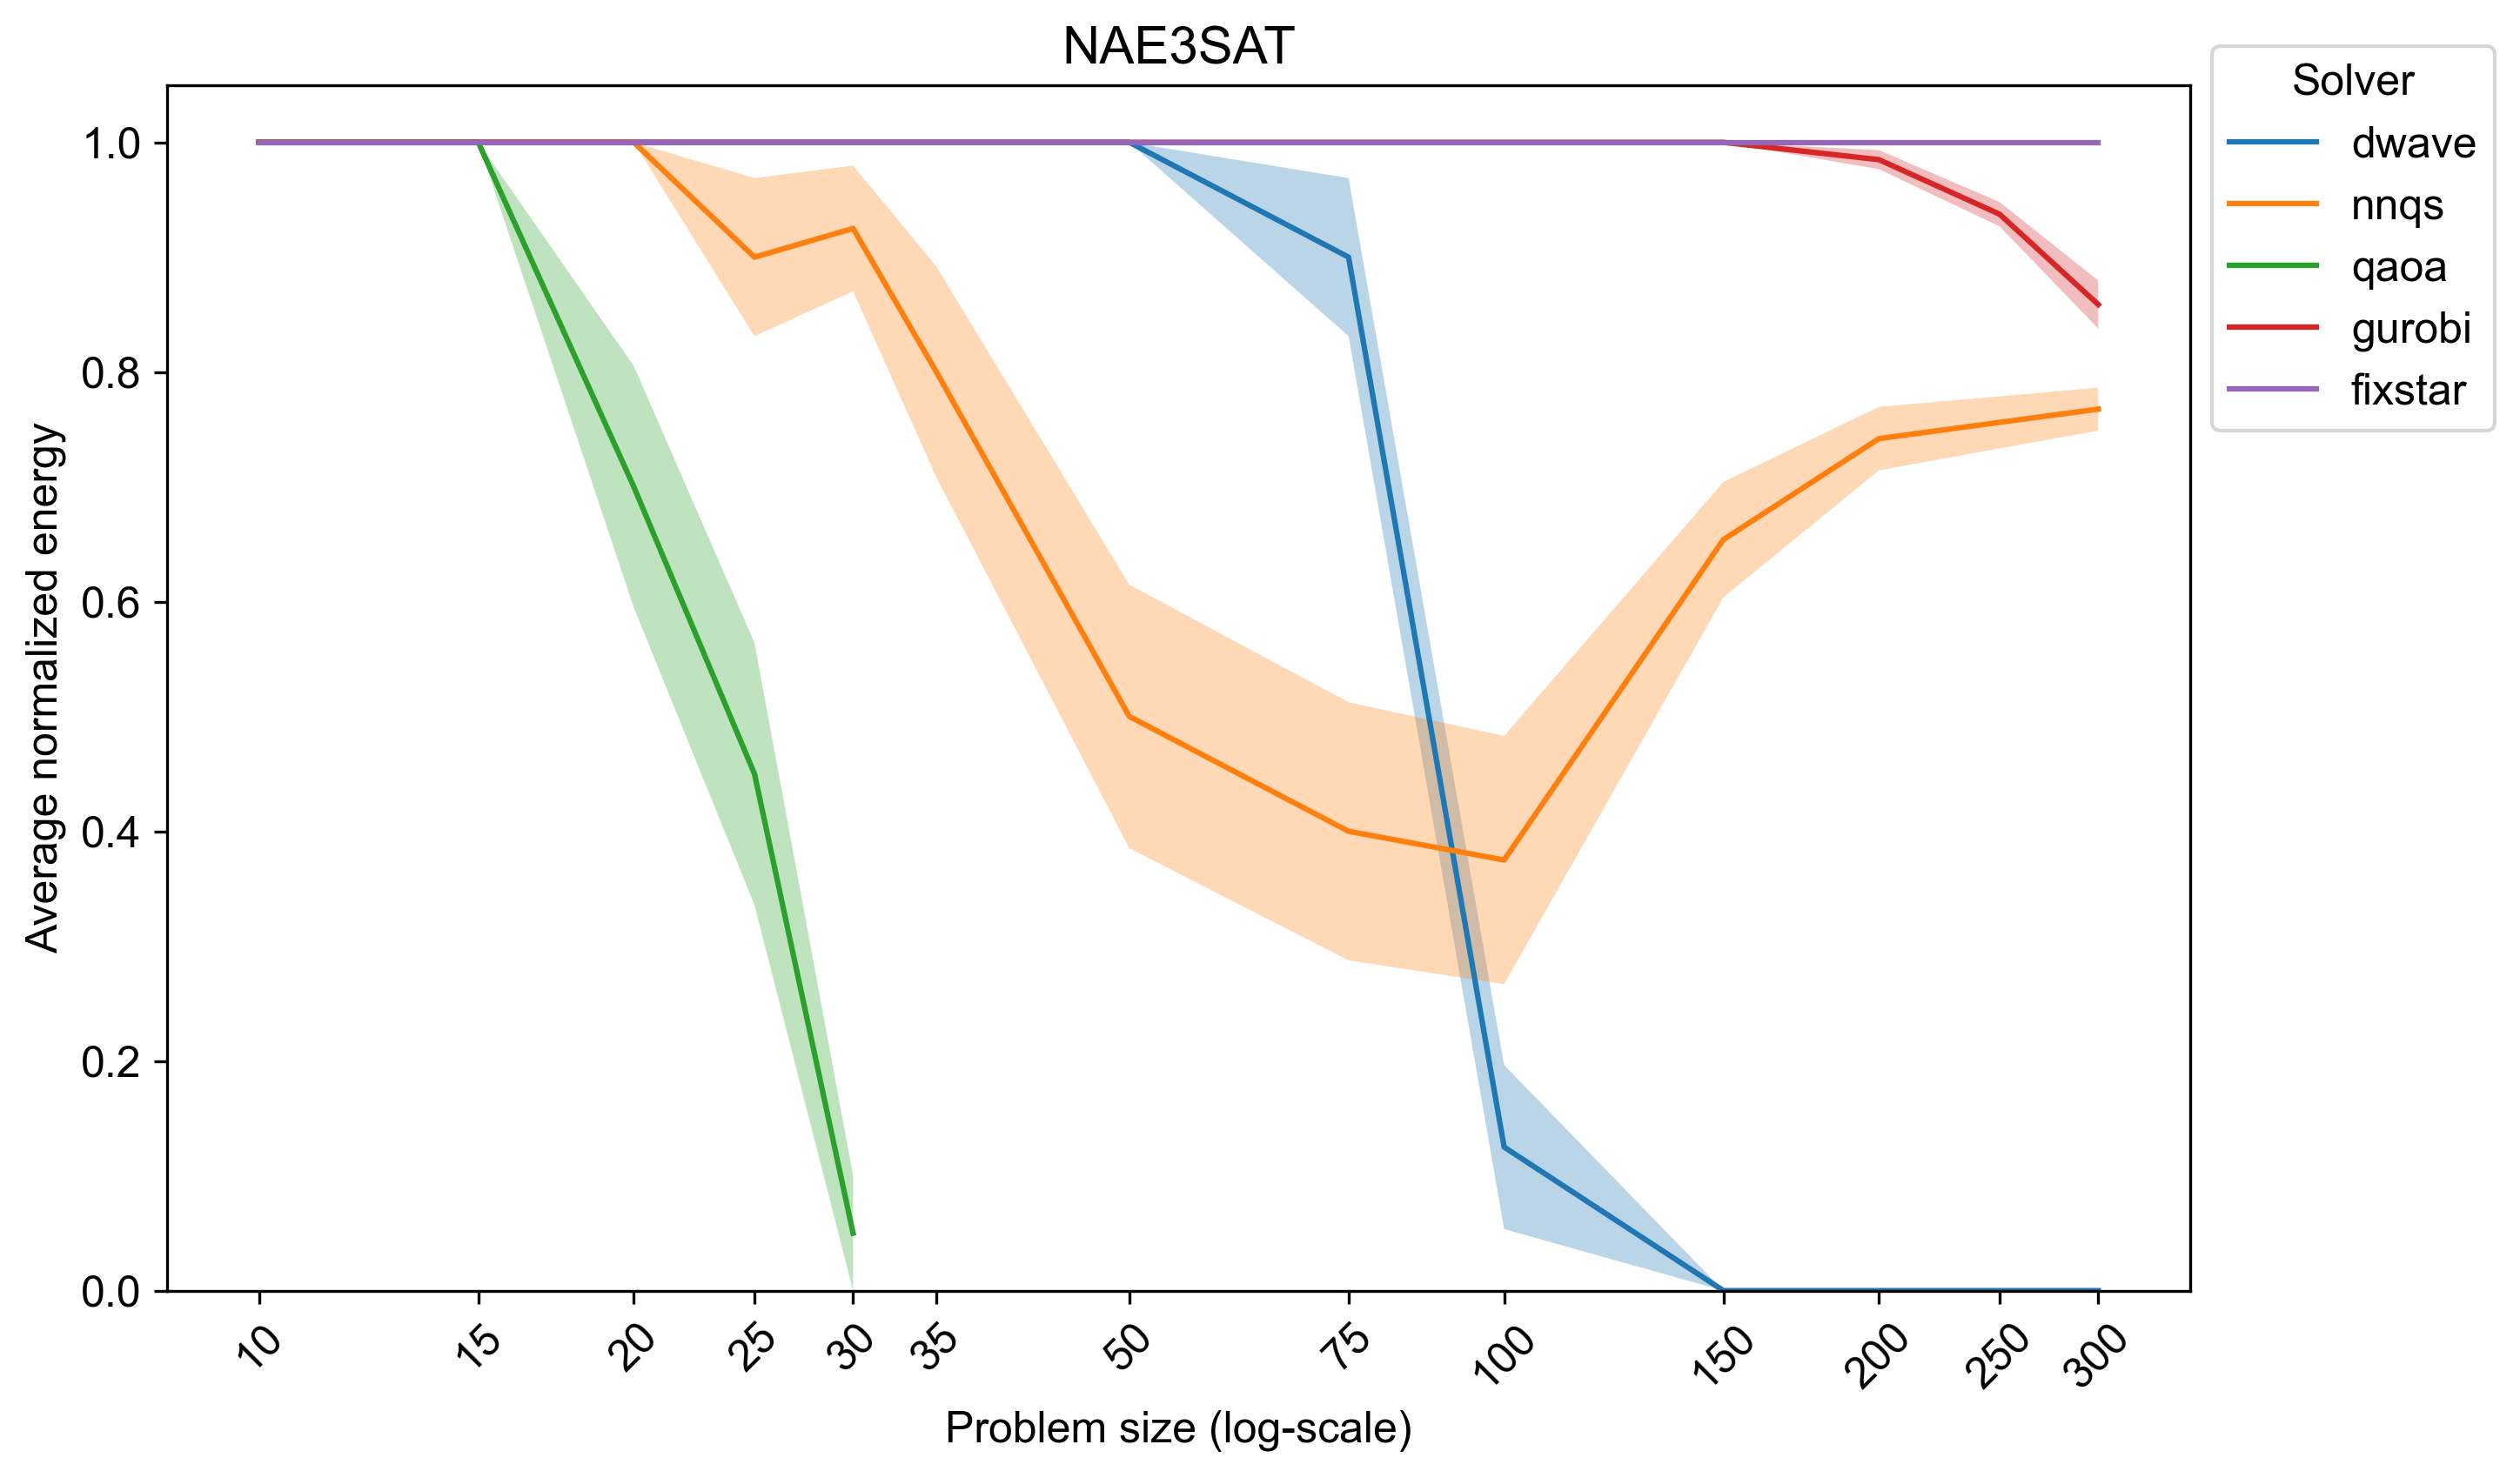
\includegraphics[width=0.9\textwidth]{images/nae3sat_all_size.png}}
    \\
    \subfloat[Success probability]{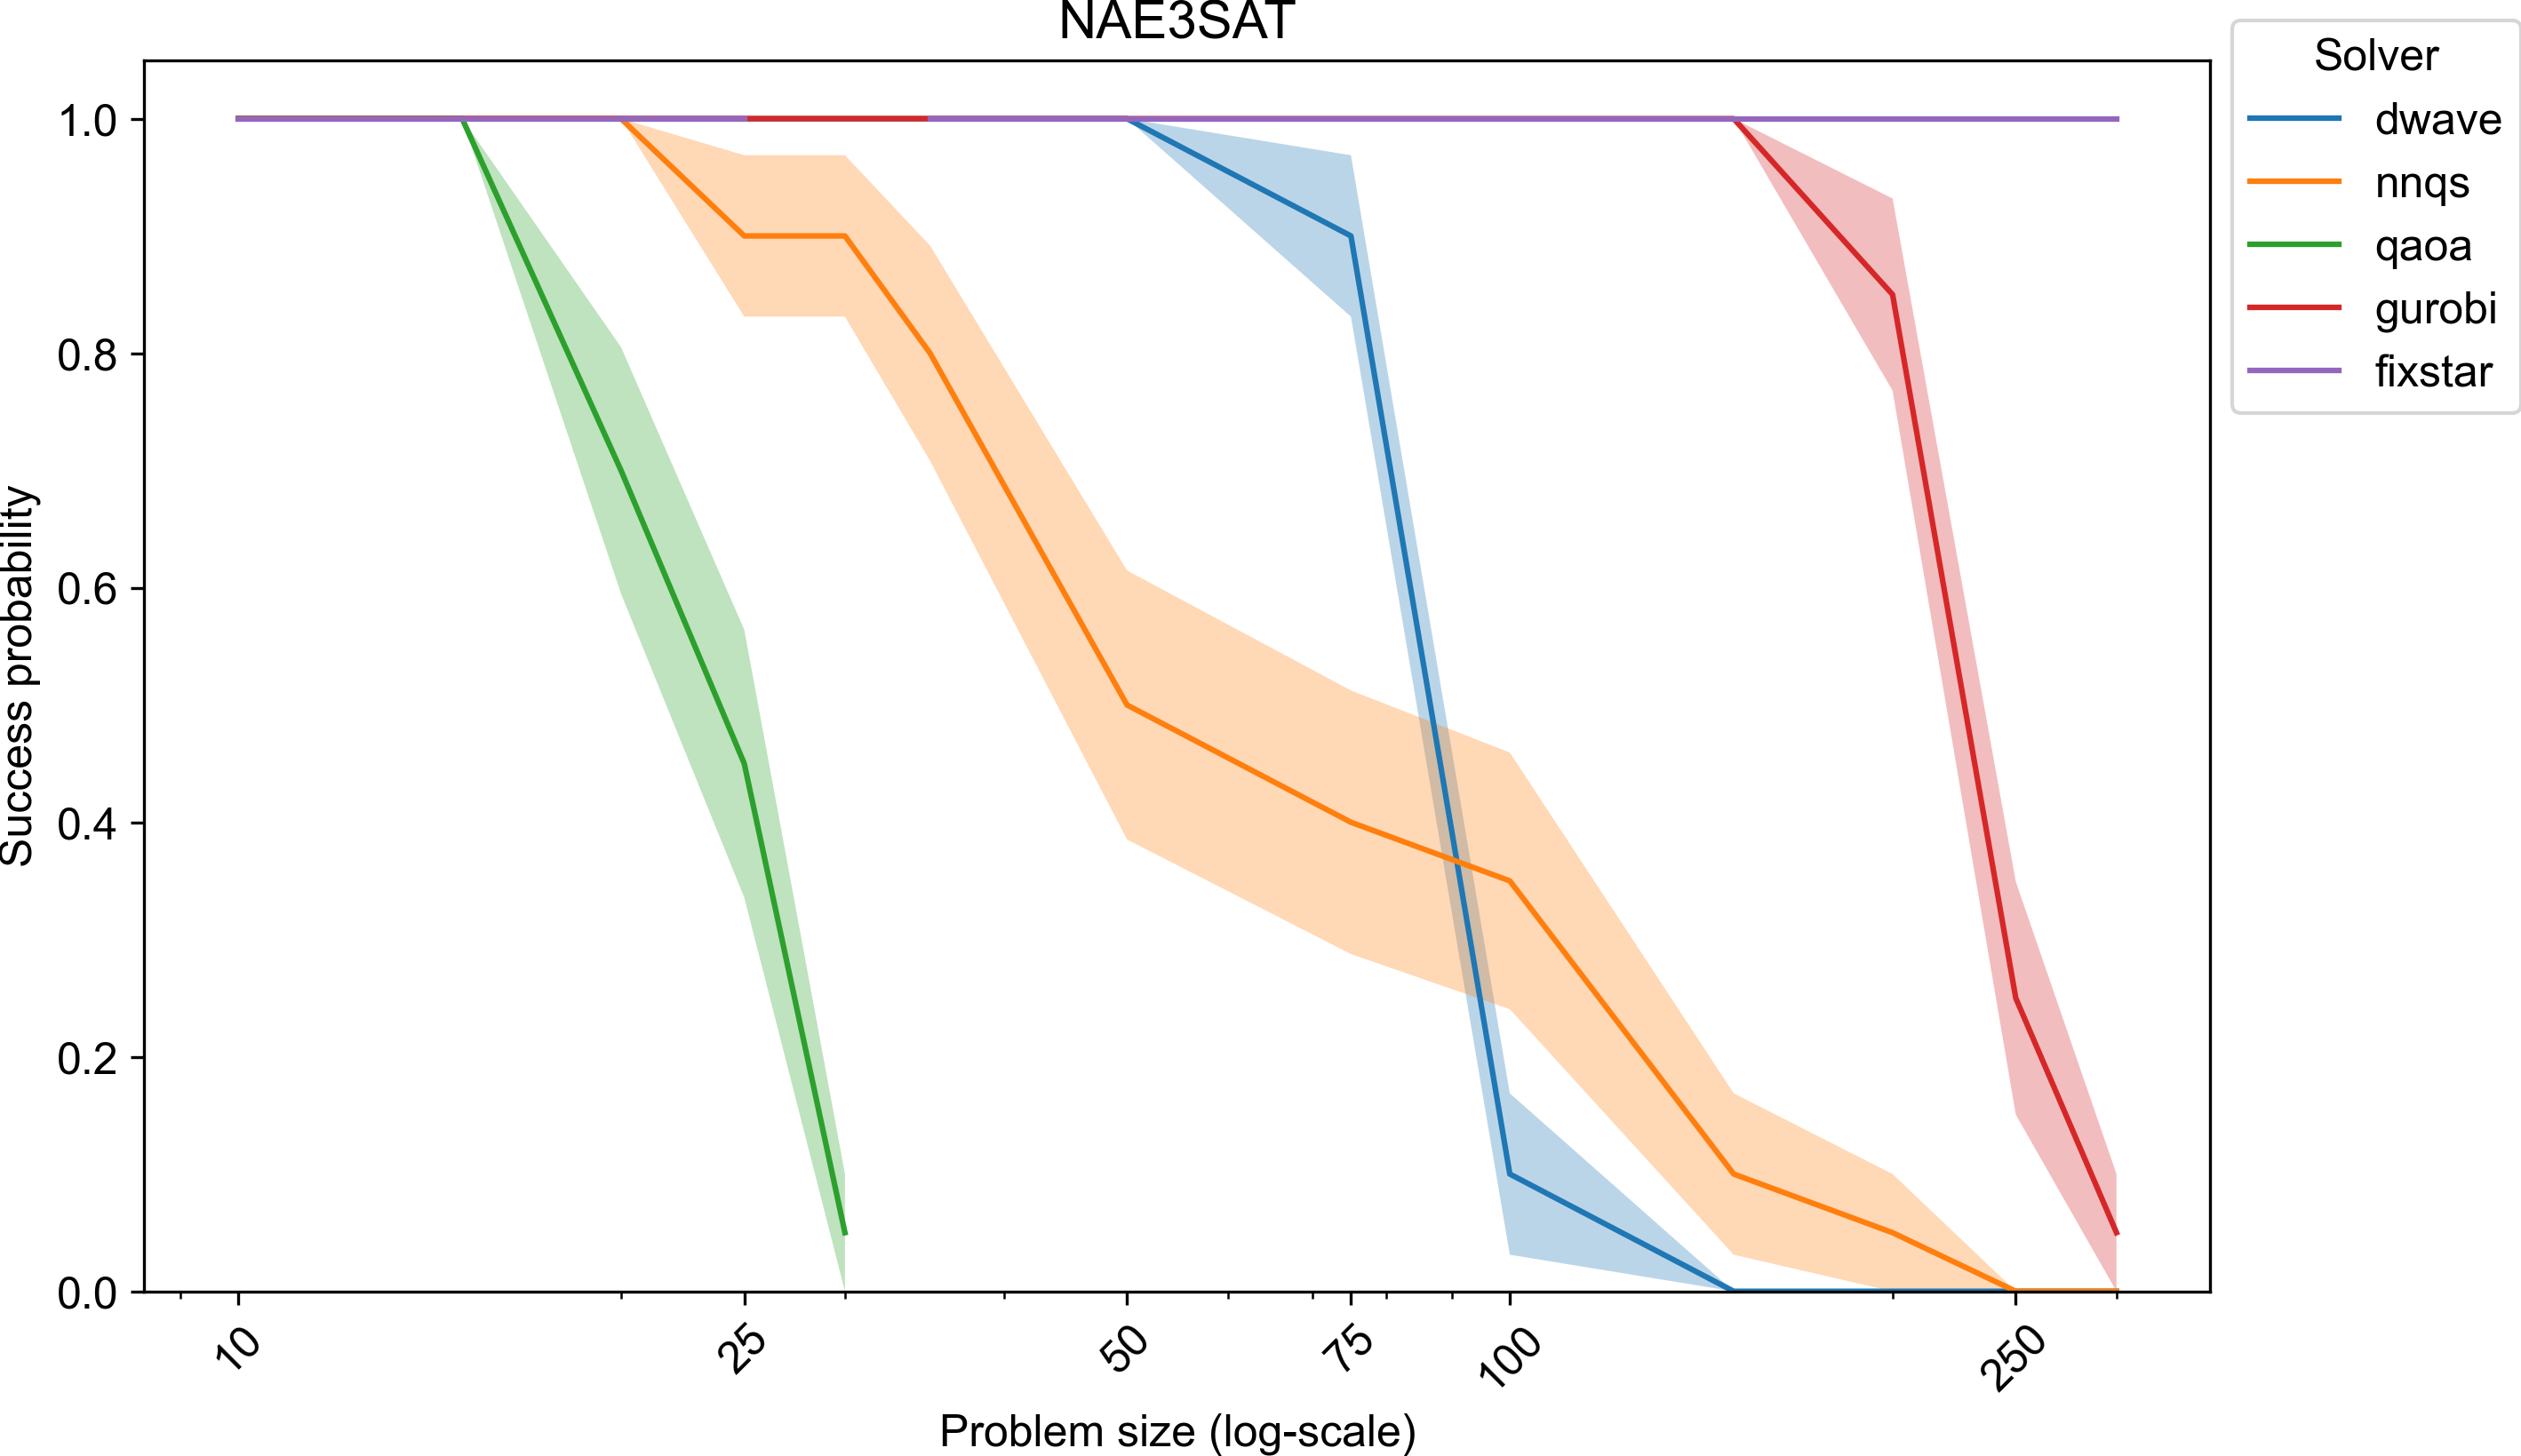
\includegraphics[width=0.9\textwidth]{images/nae3sat_all_success_size.png}}
    \caption{Performance of different solvers for NAE3SAT by problem size}
    \label{all-nae3sat-size}
\end{figure}

\begin{figure}[!htbp]
    \subfloat[Normalized energy]{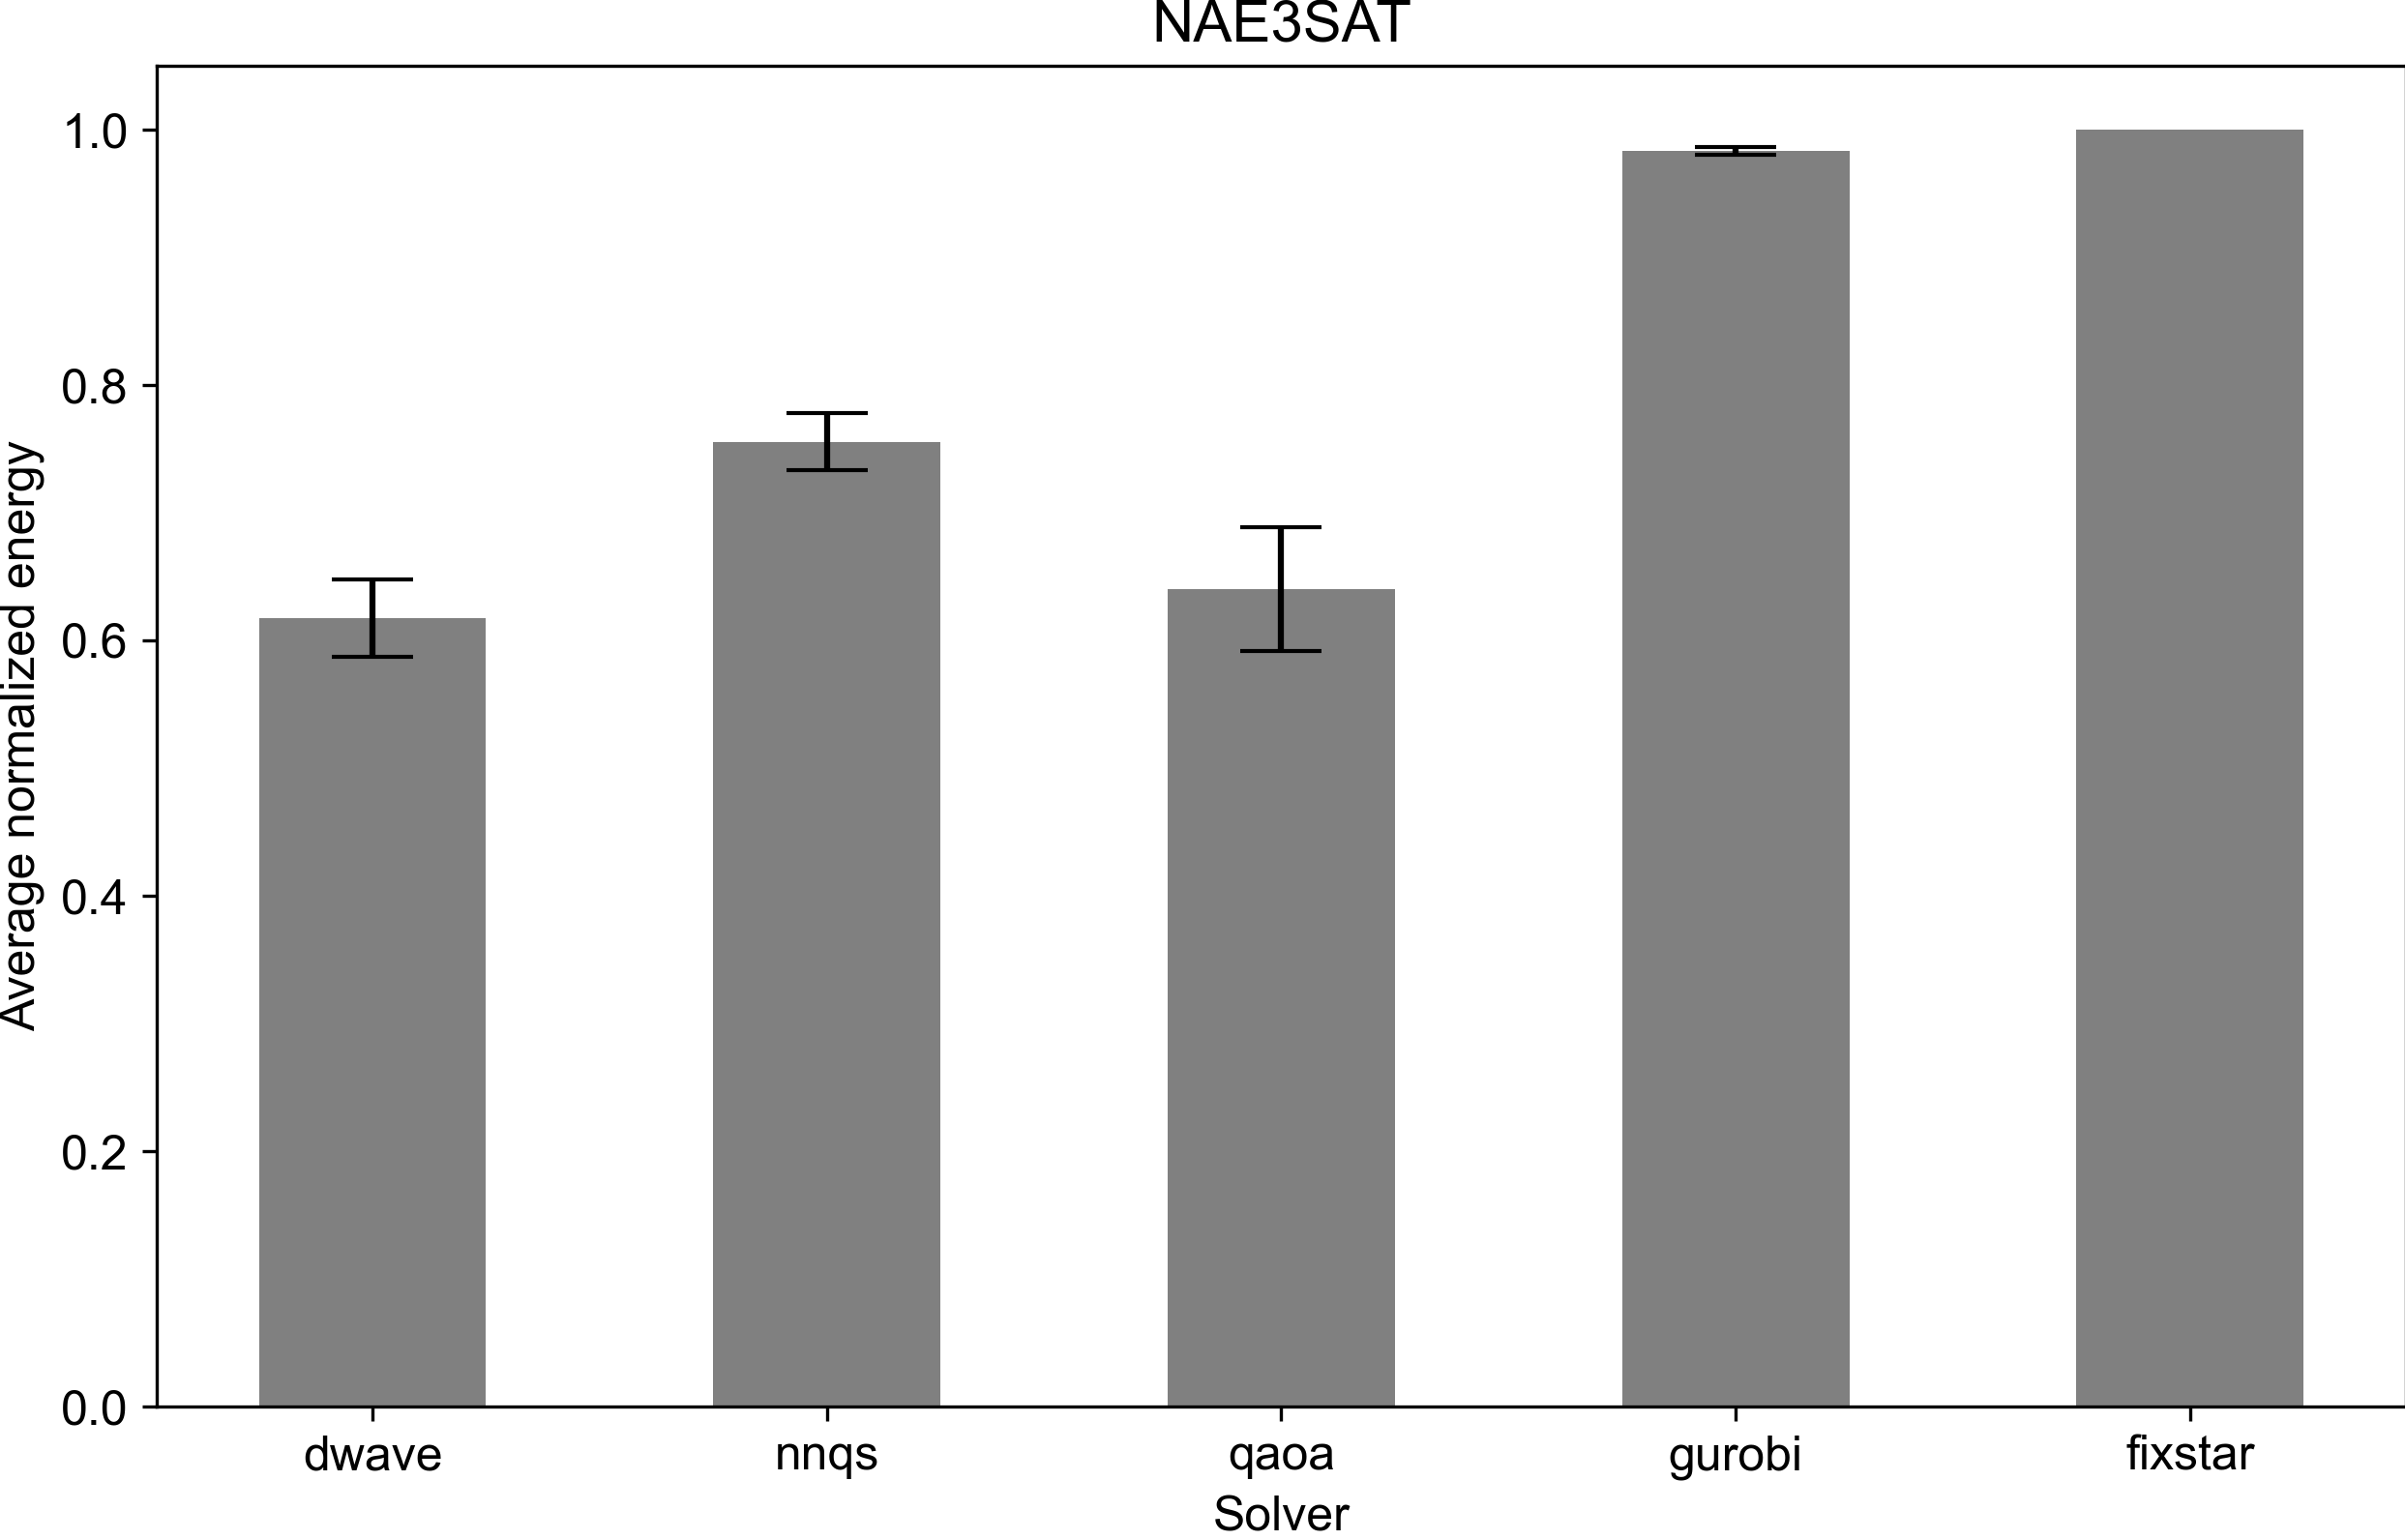
\includegraphics[width=0.49\textwidth]{images/nae3sat_all_avg.png}}\hfill
    \subfloat[Success probability]{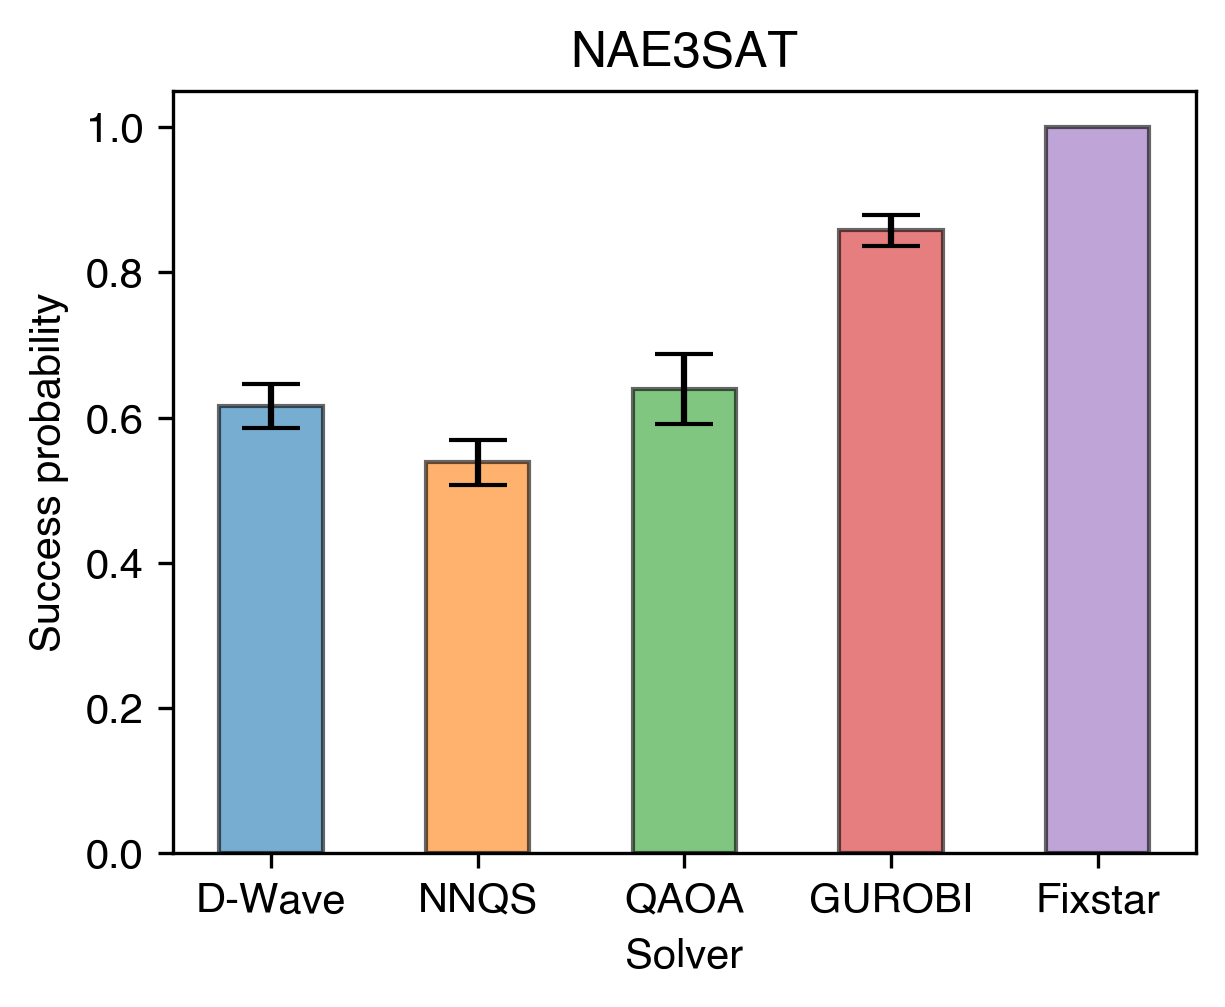
\includegraphics[width=0.49\textwidth]{images/nae3sat_all_success_avg.png}}
    \caption{Average performance of different solvers for NAE3SAT}
    \label{all-nae3sat-average}
\end{figure}

For the NAE3SAT dataset, the continuous training algorithm with the RBM performed the best in terms of normalized energy and success probability, shown in \autoref{all-nae3sat-size}, except with a problem size of $50$. This is likely due to variance in the randomly generated data set. The performance averaged across all sizes, shown in \autoref{all-nae3sat-average}, also highlights that the RBM with a continuous training algorithm performs the best.

\subsection{Max-cut}

\begin{figure}[!htbp]
    \subfloat[Normalized energy]{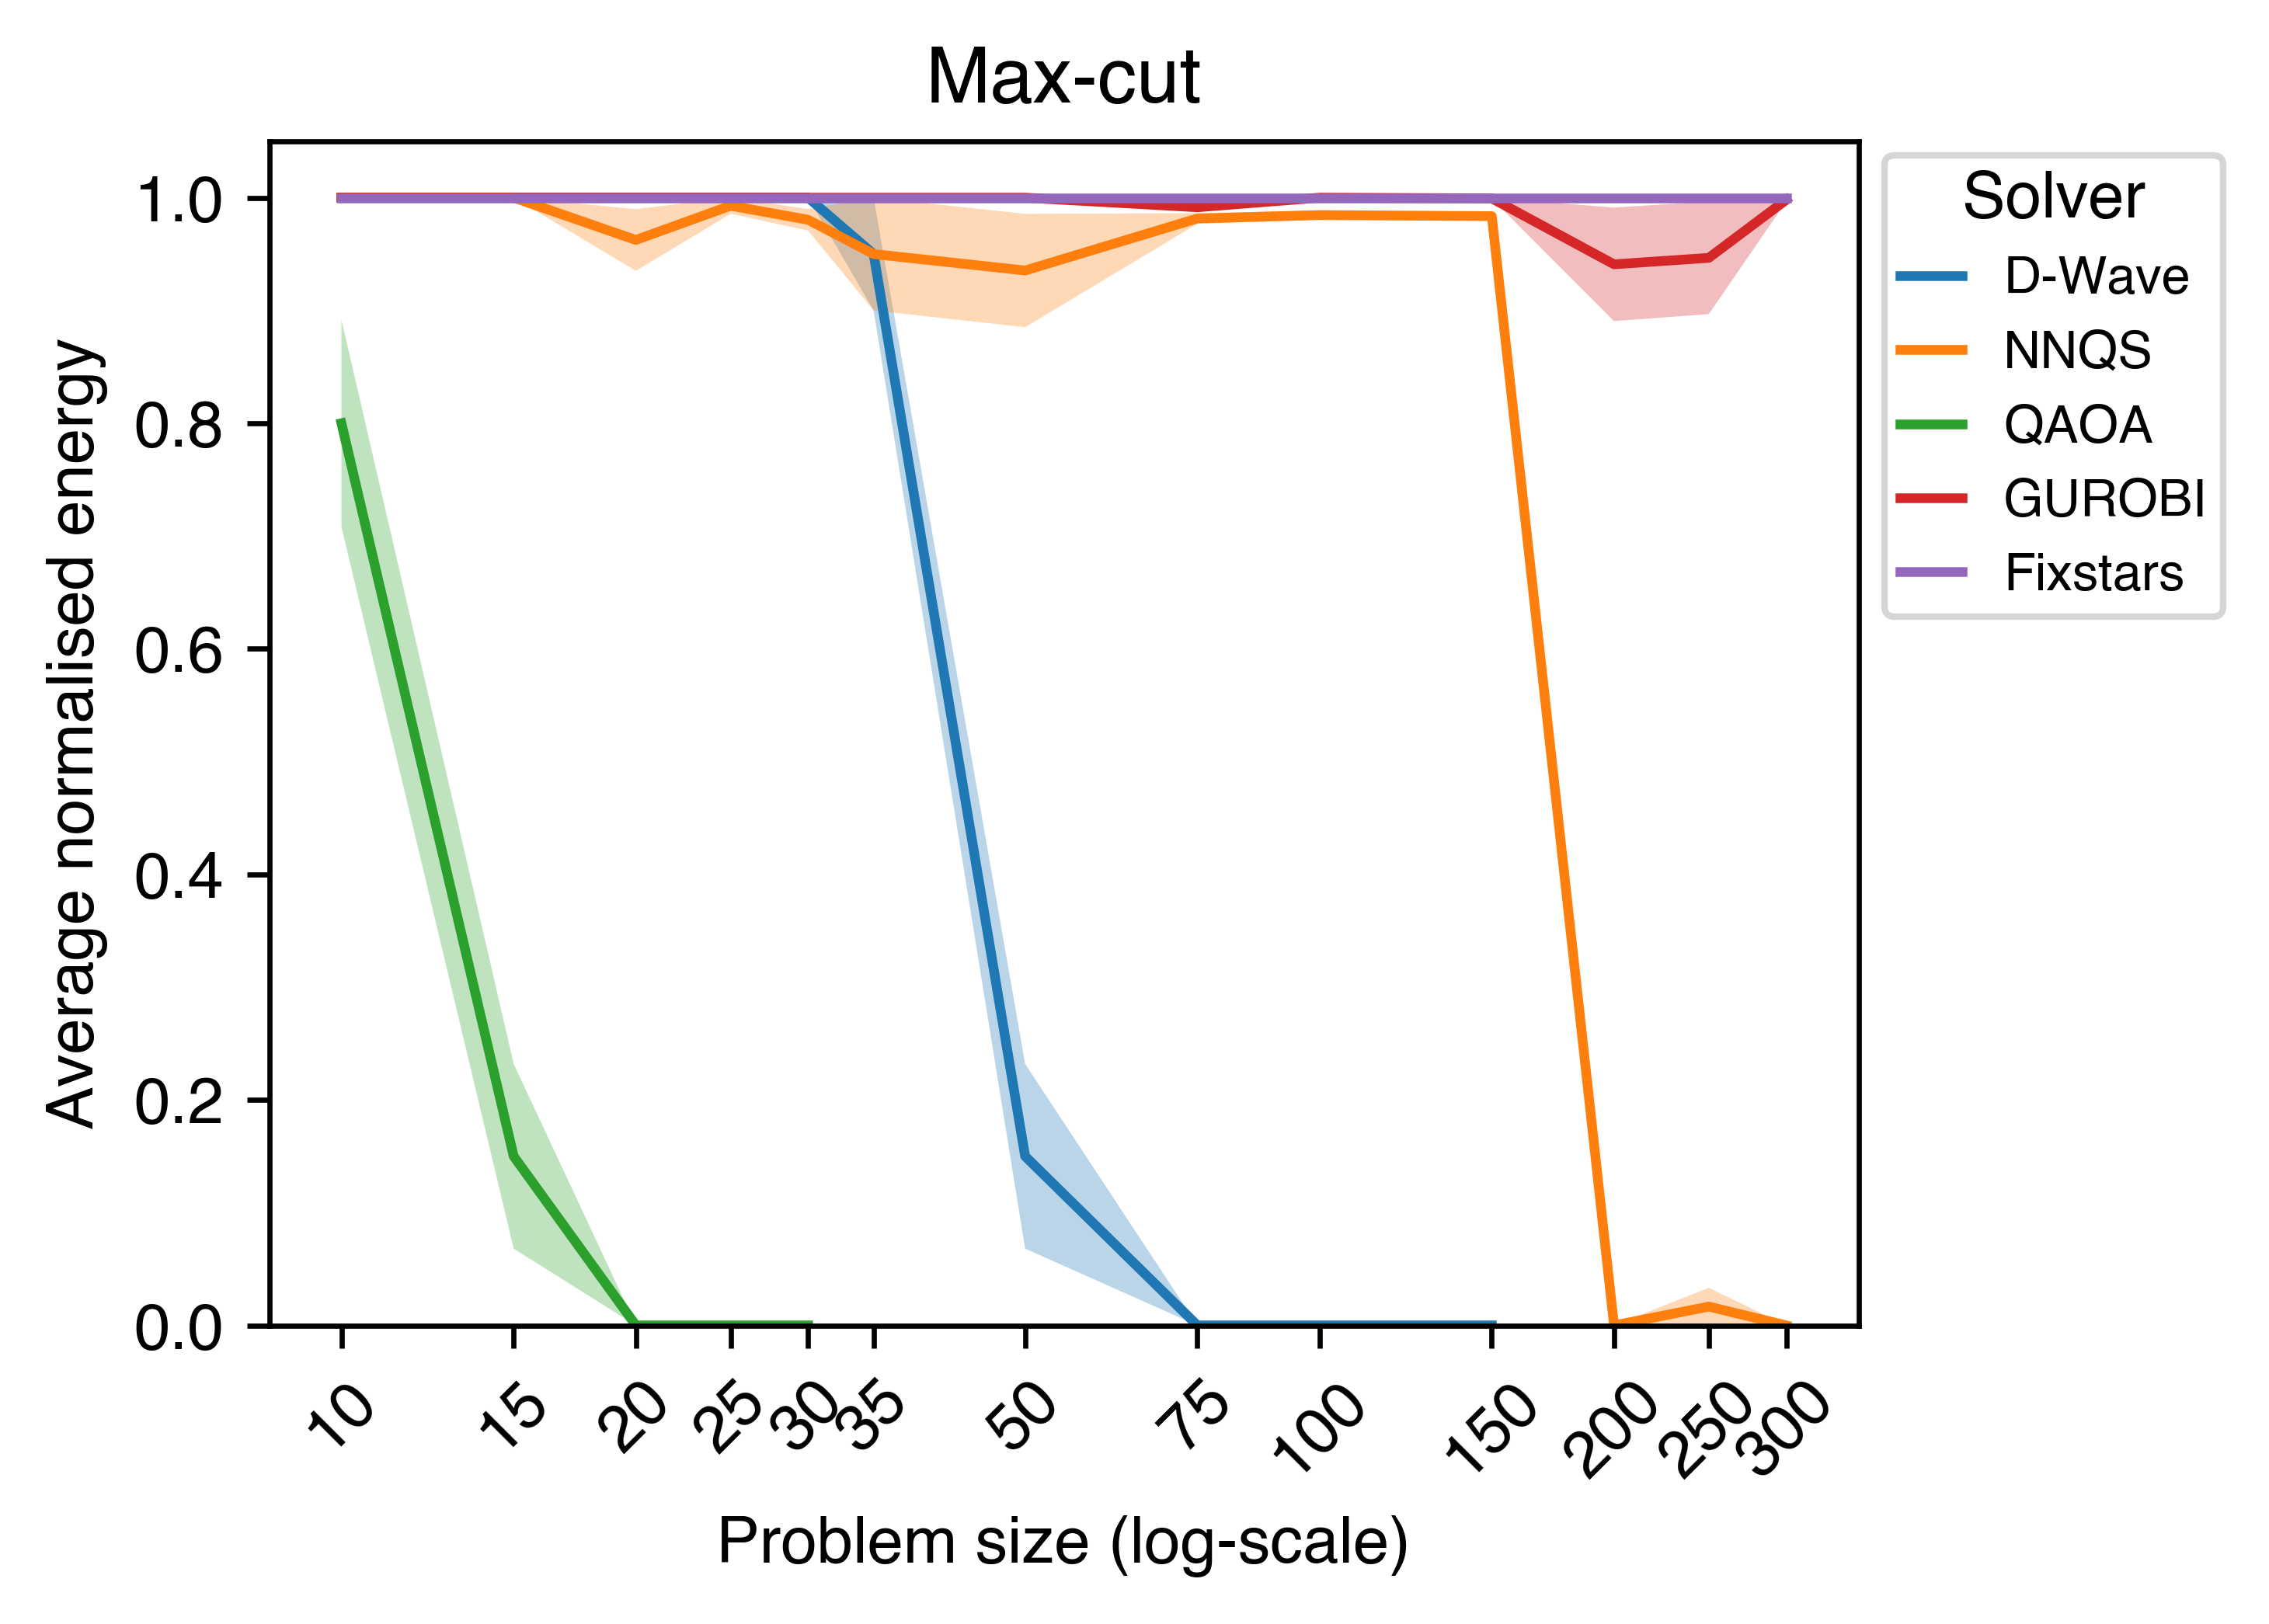
\includegraphics[width=0.9\textwidth]{images/maxcut_all_size.png}}
    \\
    \subfloat[Success probability]{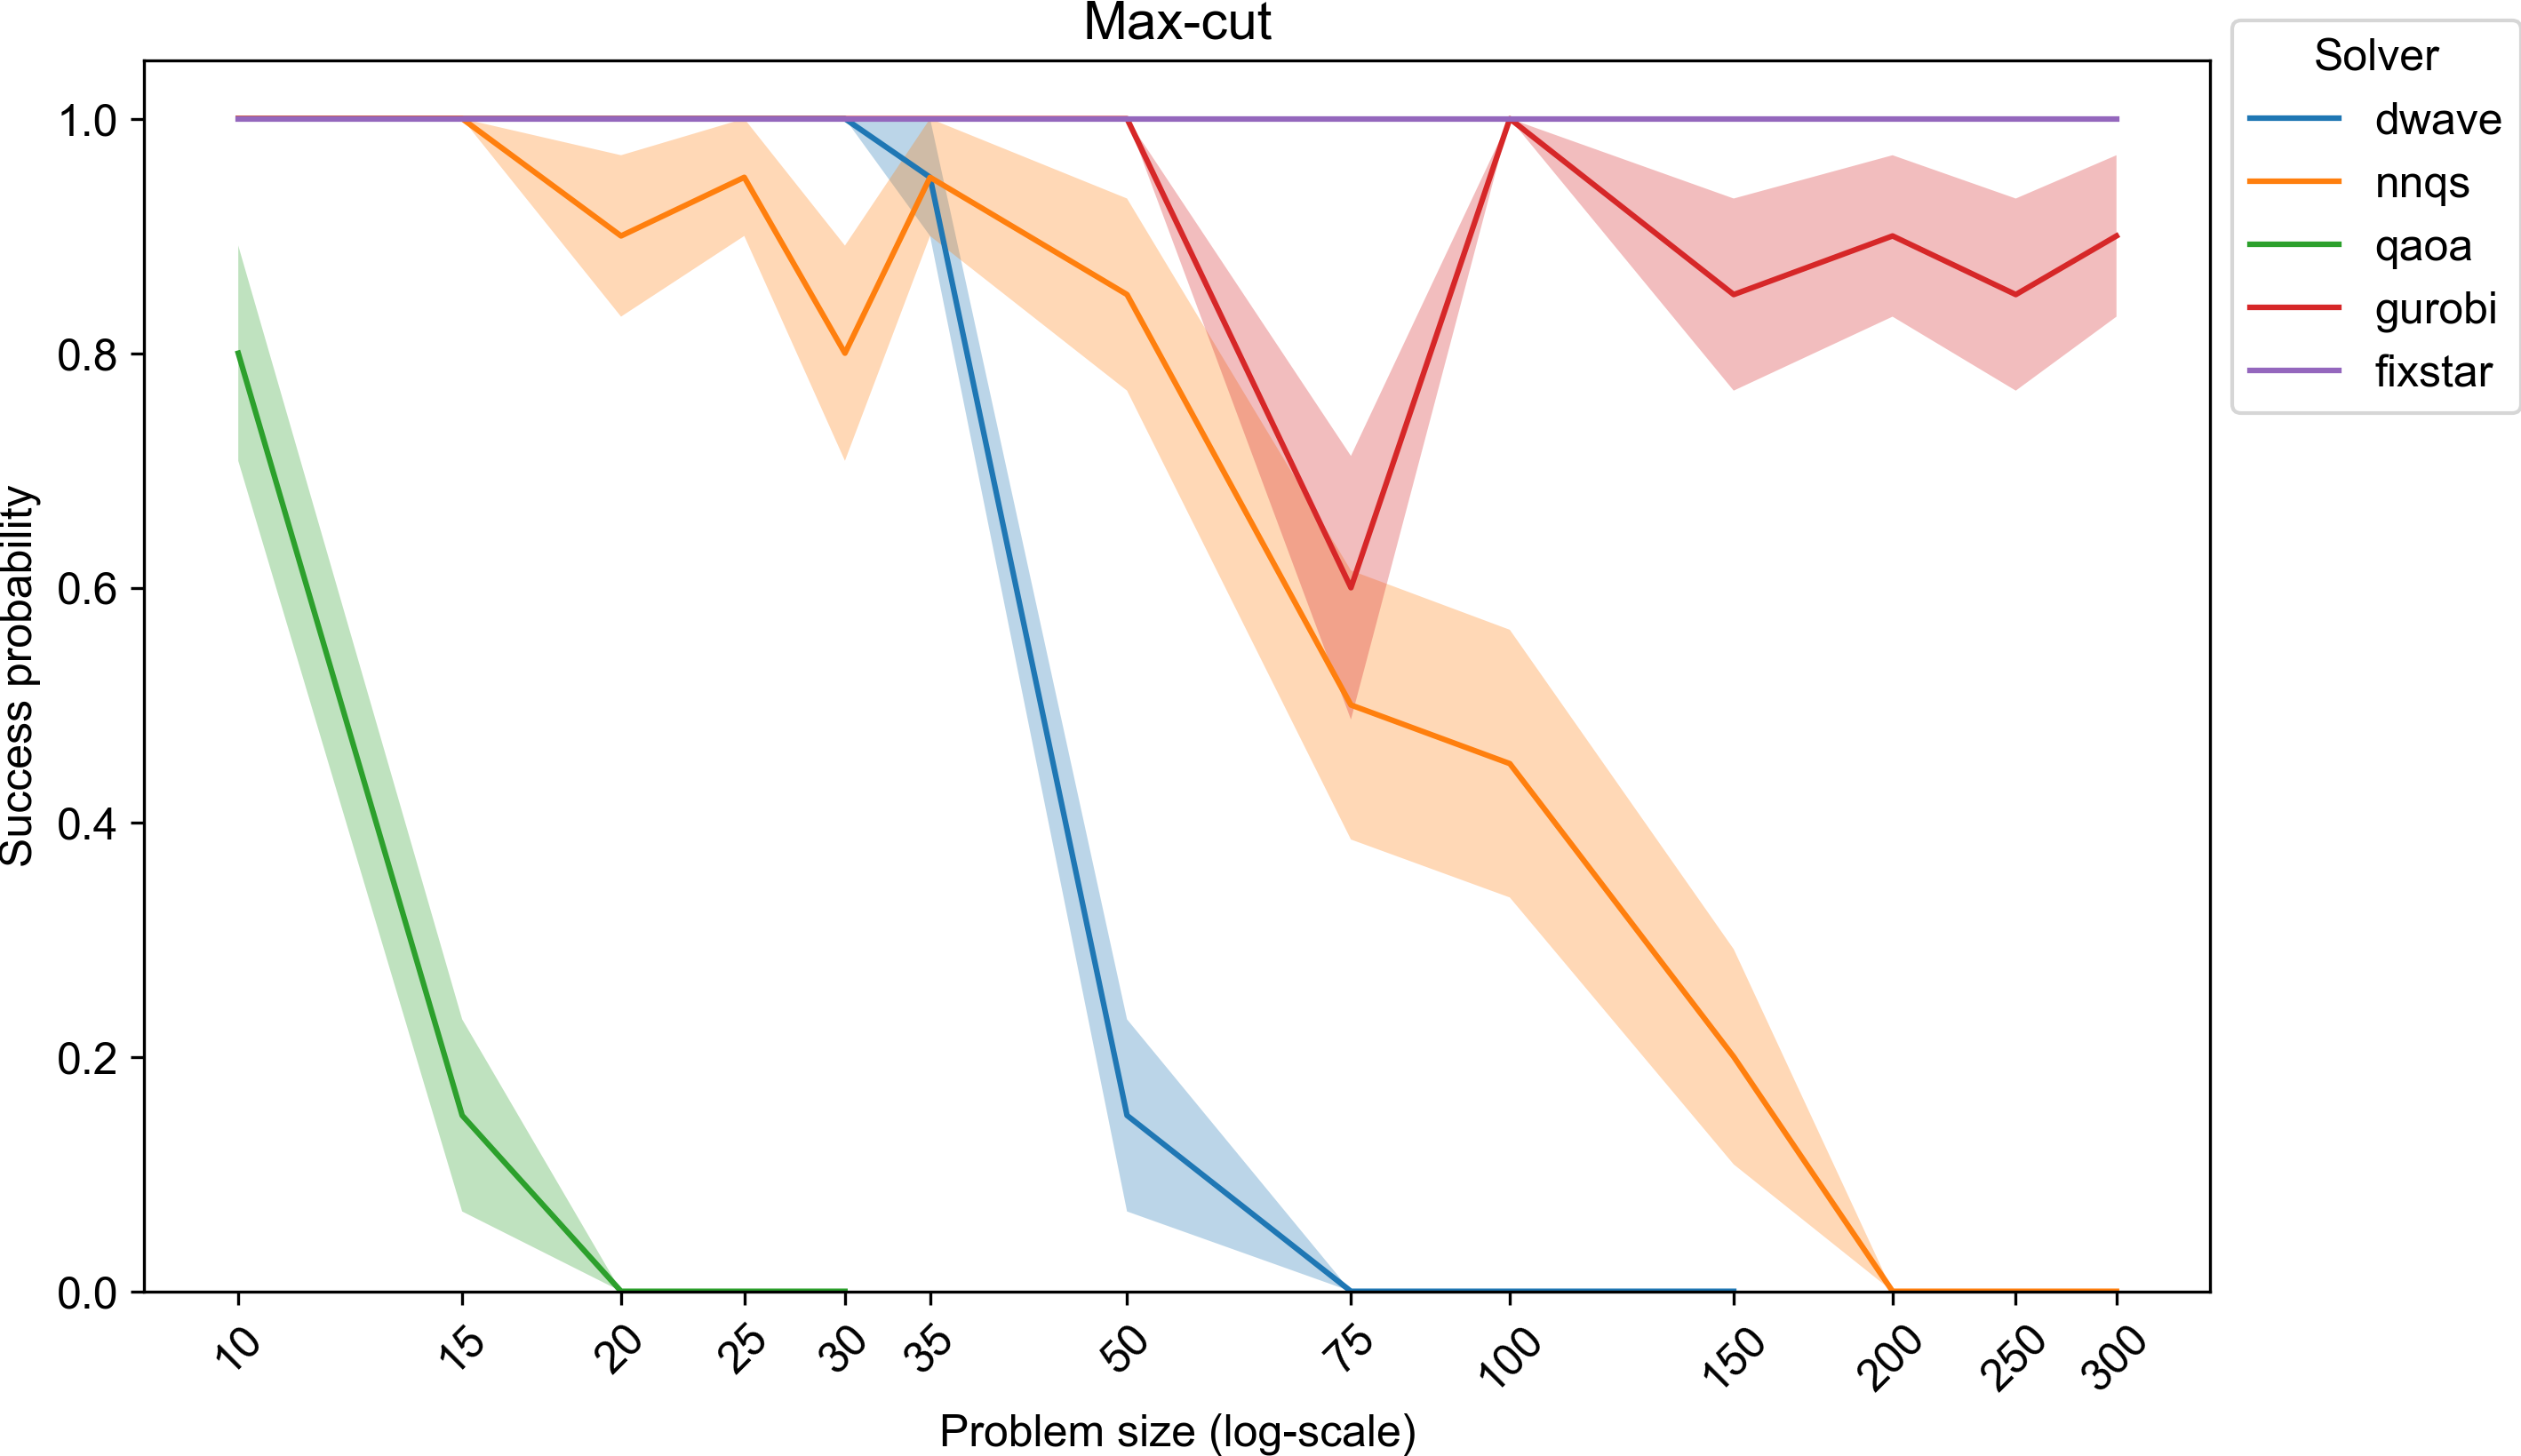
\includegraphics[width=0.9\textwidth]{images/maxcut_all_success_size.png}}
    \caption{Performance of different solvers for max-cut by problem size}
    \label{all-maxcut-size}
\end{figure}

\begin{figure}[!htbp]
    \subfloat[Normalized energy]{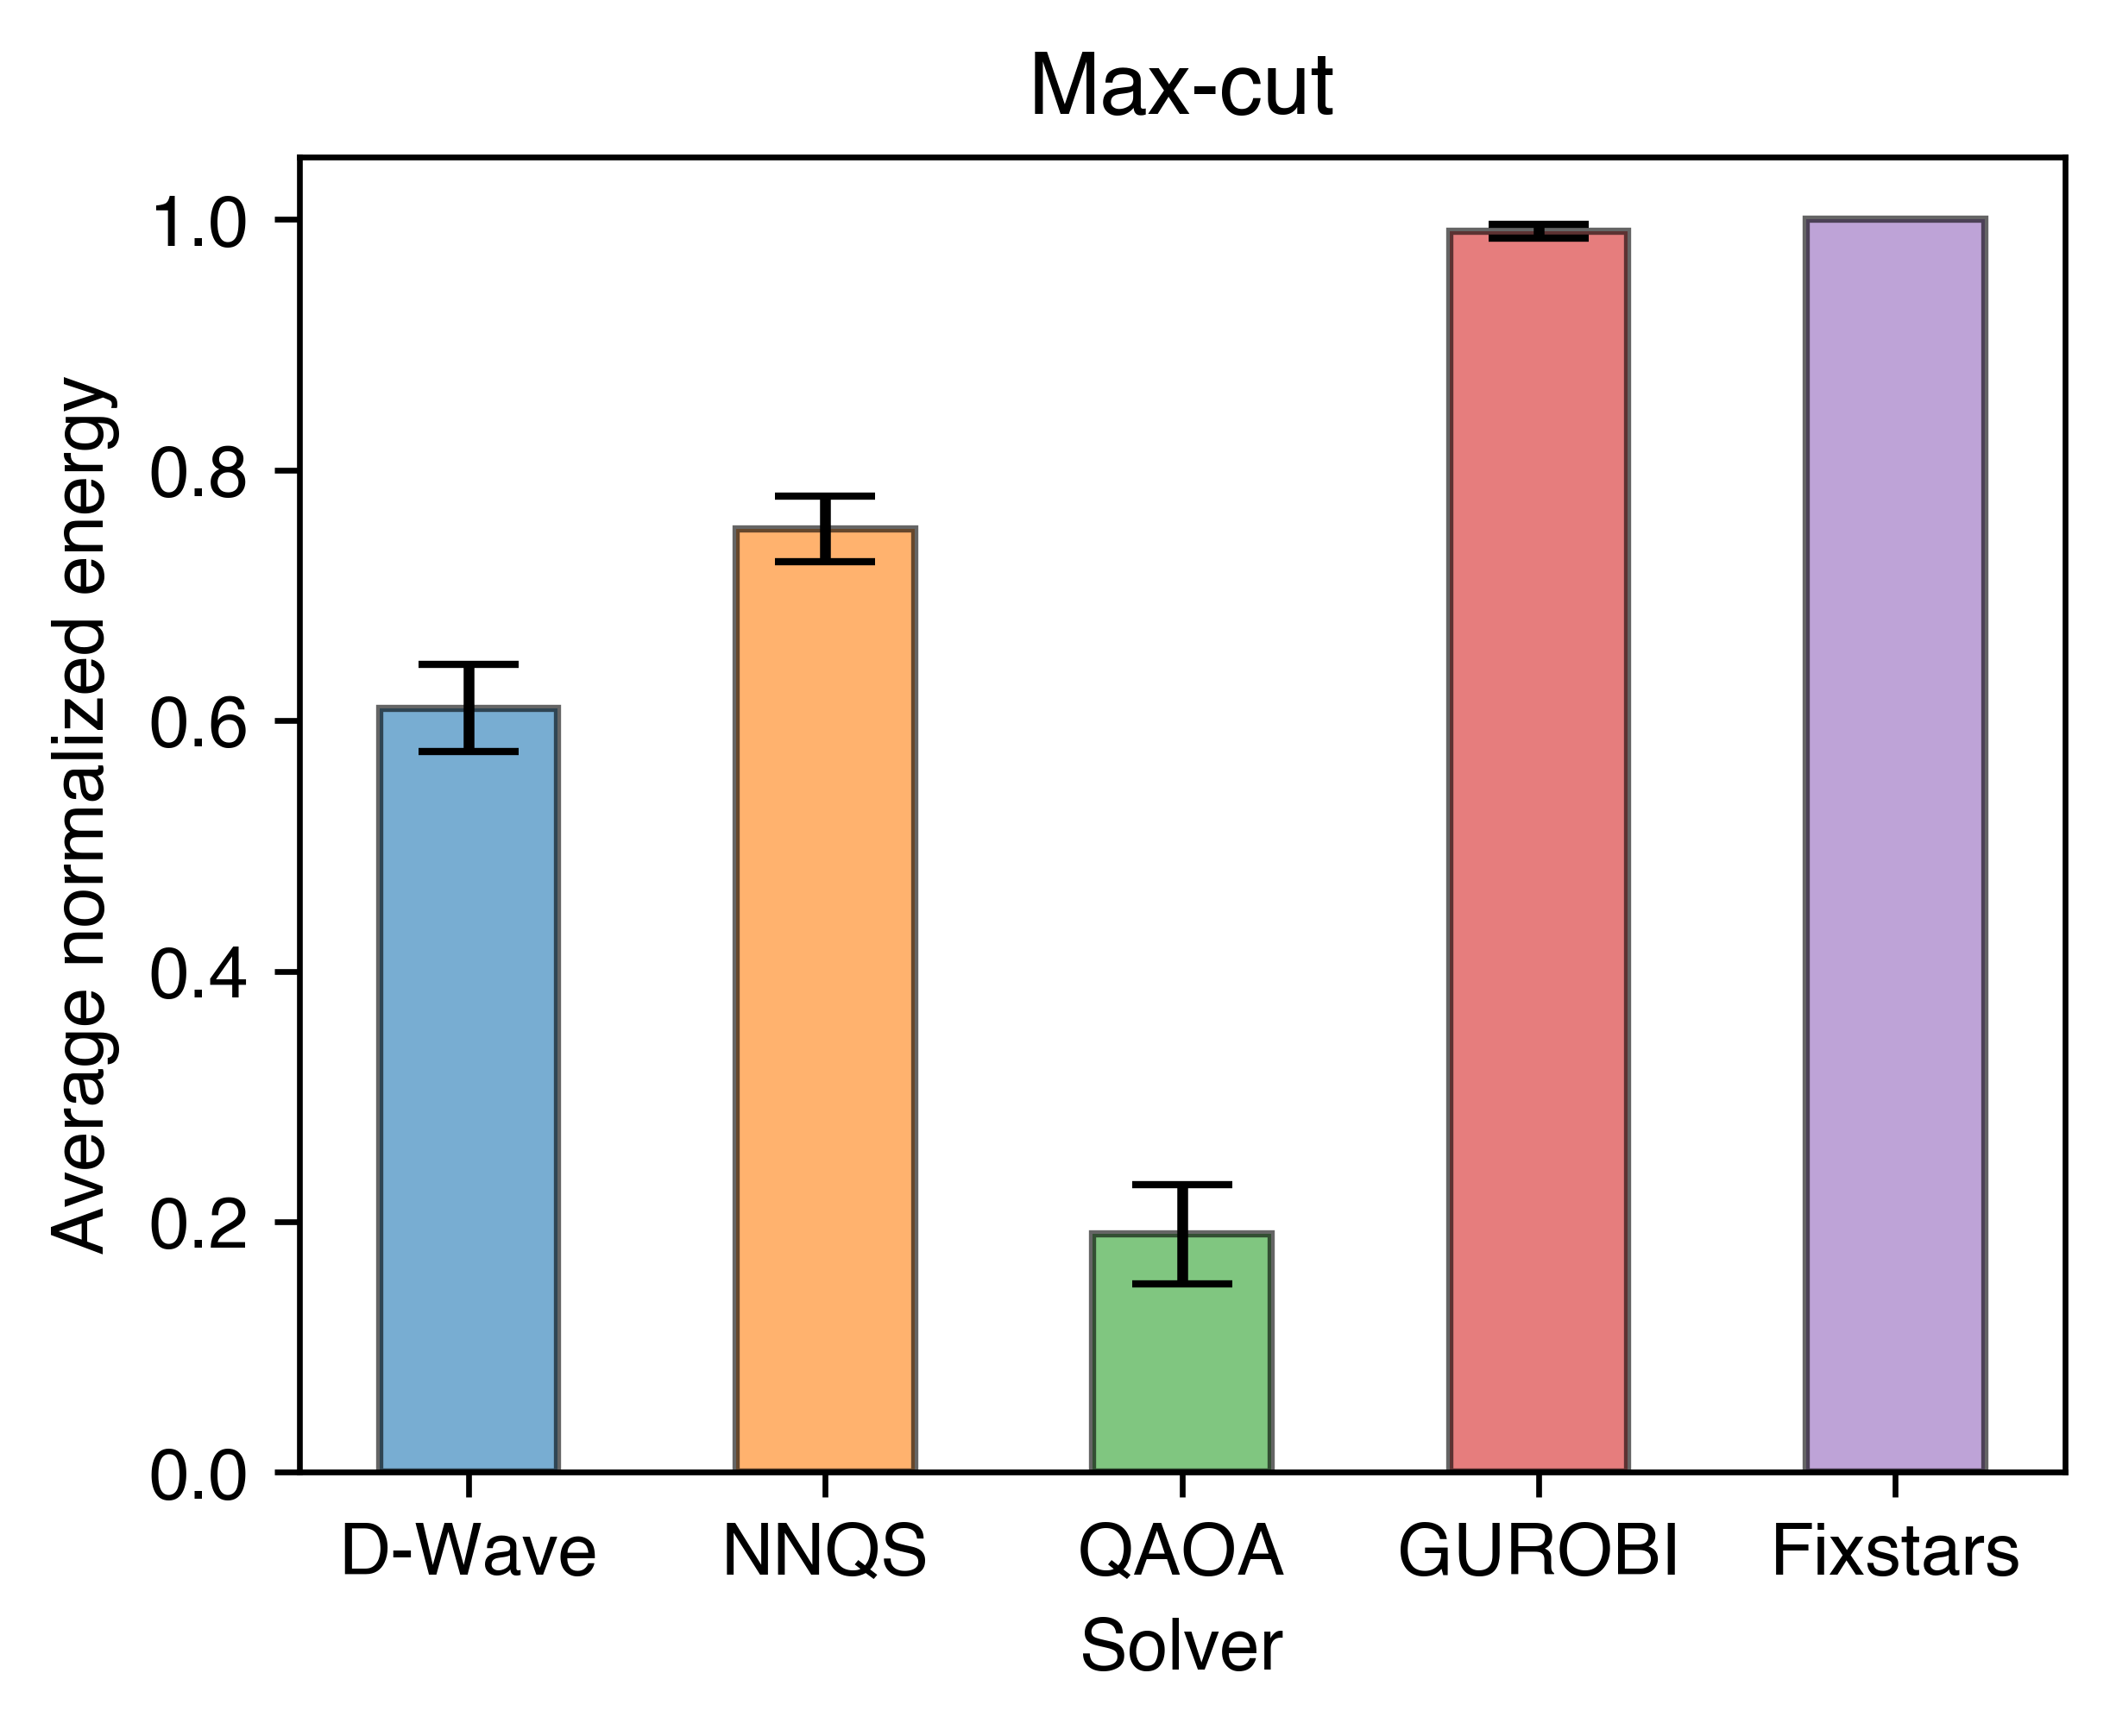
\includegraphics[width=0.49\textwidth]{images/maxcut_all_avg.png}}\hfill
    \subfloat[Success probability]{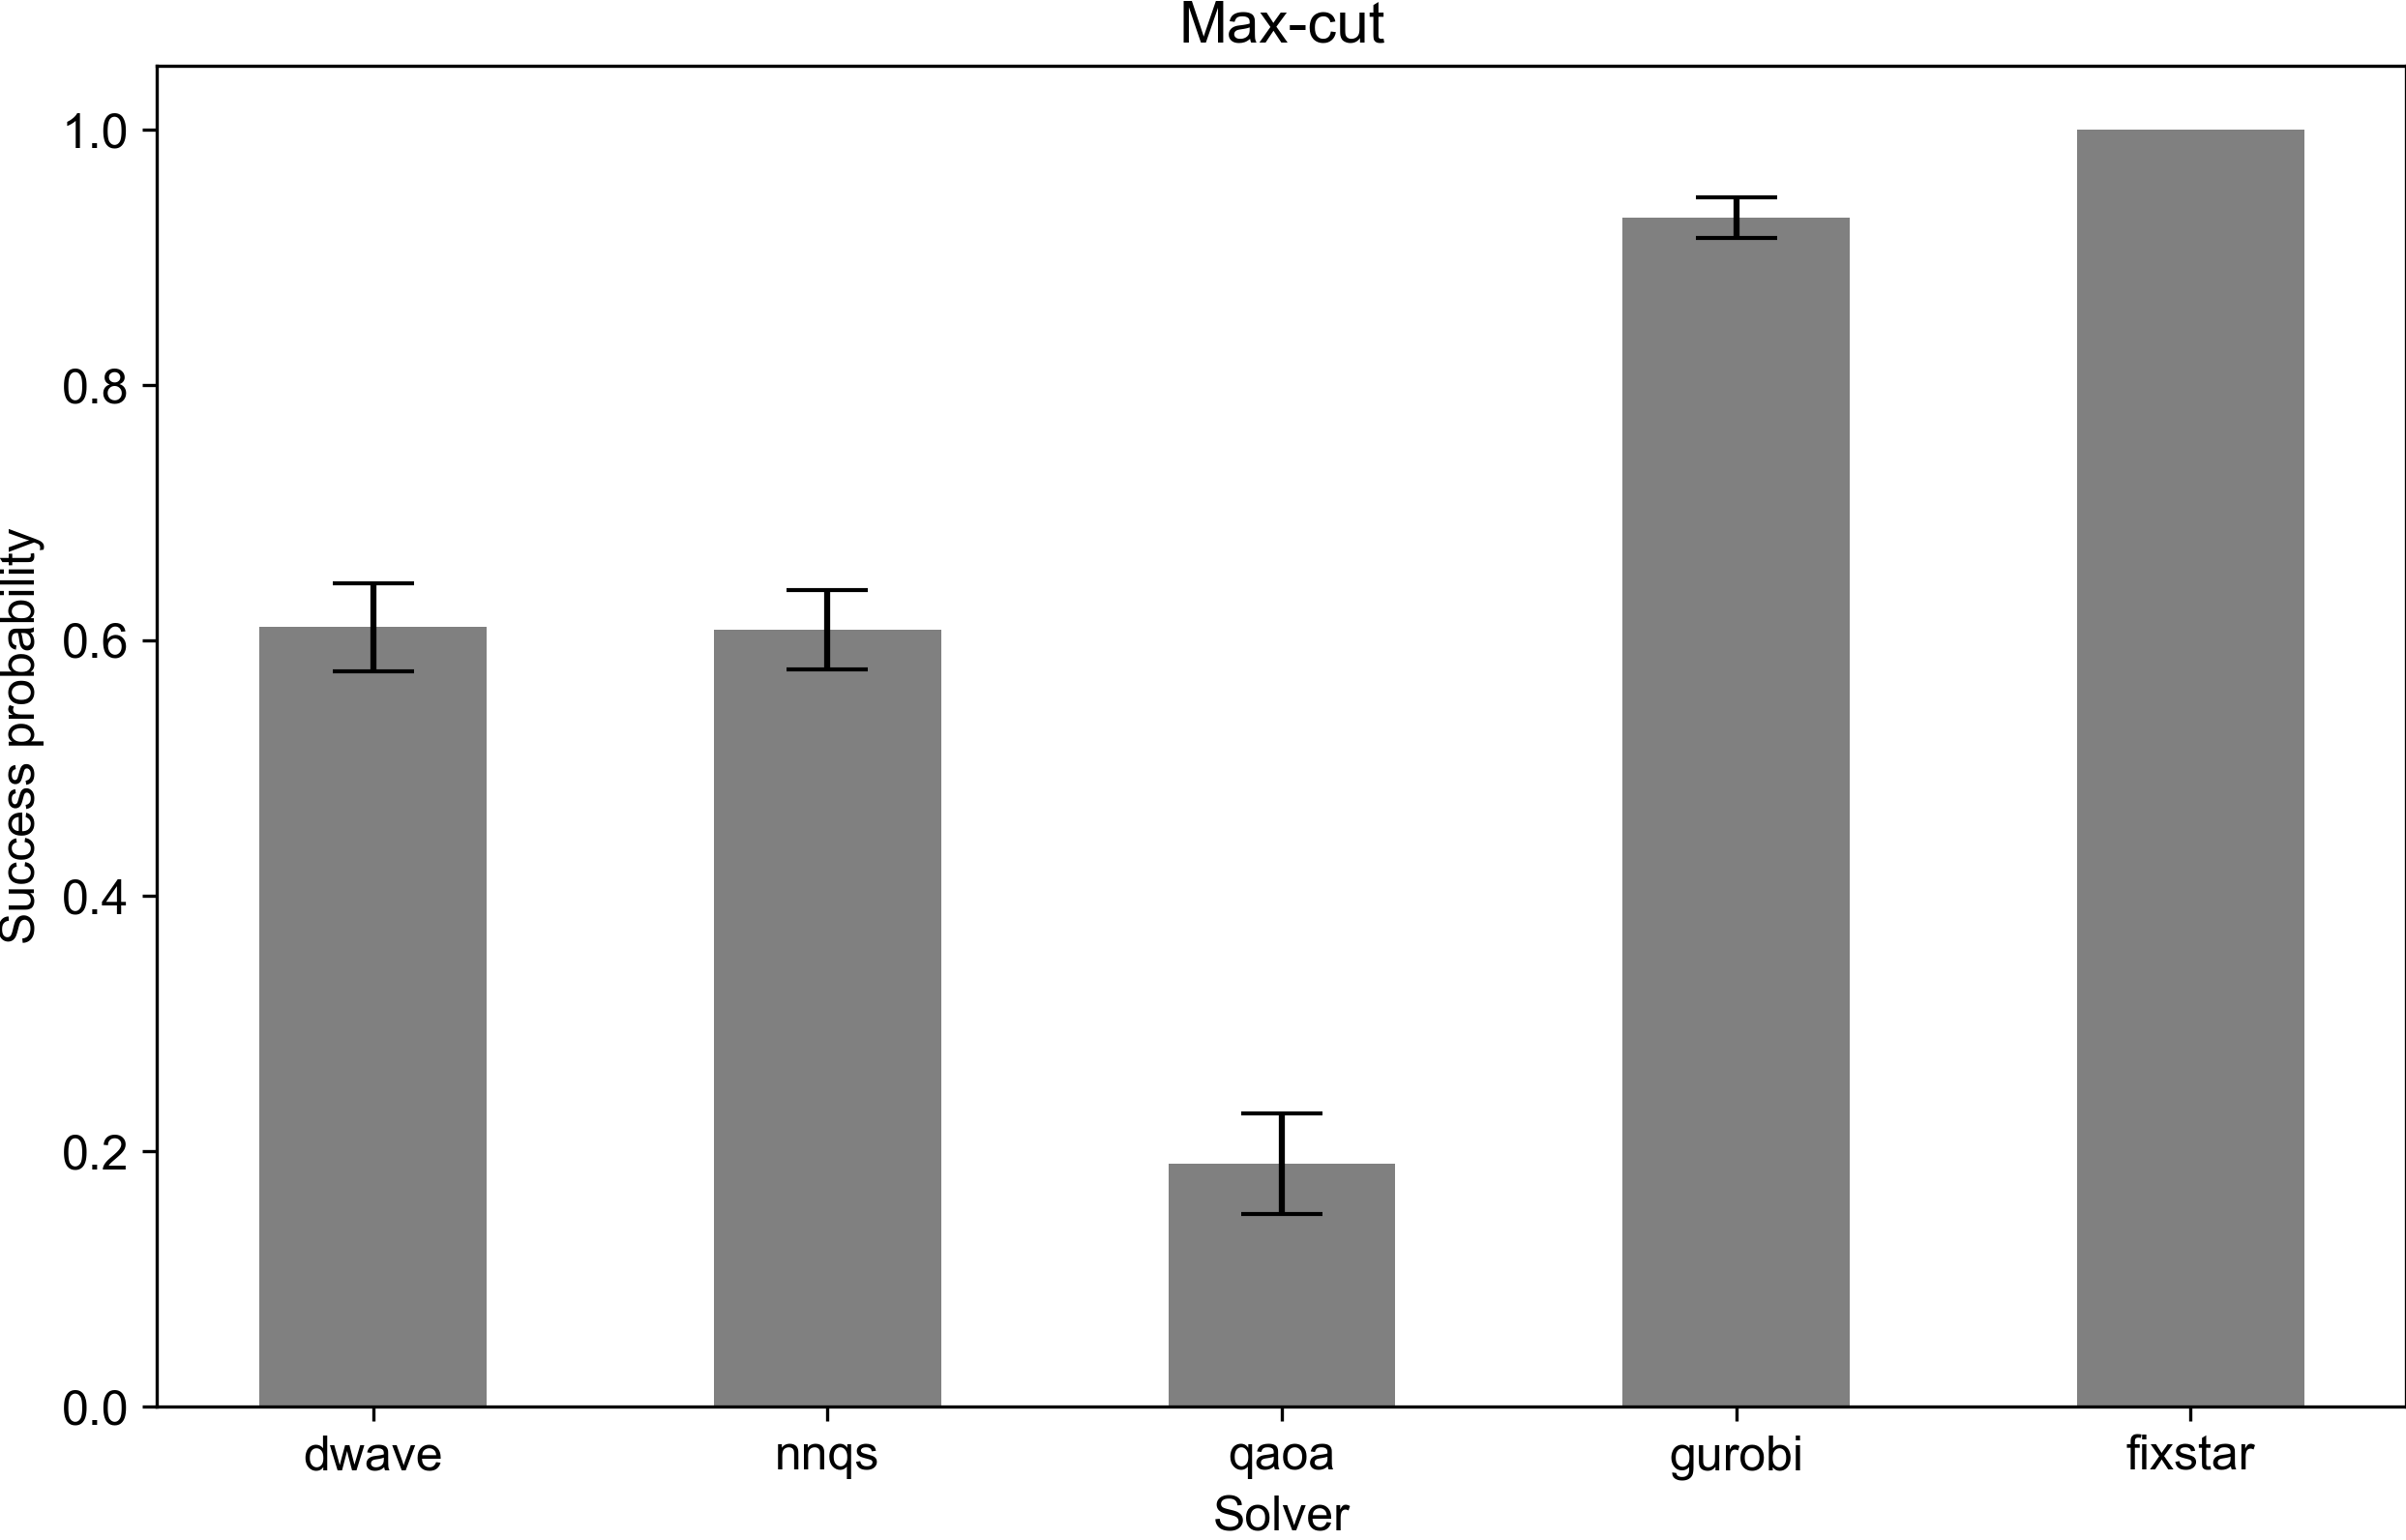
\includegraphics[width=0.49\textwidth]{images/maxcut_all_success_avg.png}}
    \caption{Average performance of different solvers for max-cut}
    \label{all-maxcut-average}
\end{figure}

For the max-cut dataset, the continuous training algorithm with the RBM generally performed the best in terms of normalized energy and success probability, shown in \autoref{all-maxcut-size}, except with a problem size of $25$. This is likely due to variance in the randomly generated data set. The performance averaged across all sizes, shown in \autoref{all-maxcut-average}, also highlights that the RBM with a continuous training algorithm performs the best. However, the gap in success probability between the models is relatively small and this likely implies that the max-cut problem is easier in general compared to the NAE3SAT problem.


\subsection{SK model}

\begin{figure}[!htbp]
    \centering
    \subfloat[Normalized energy]{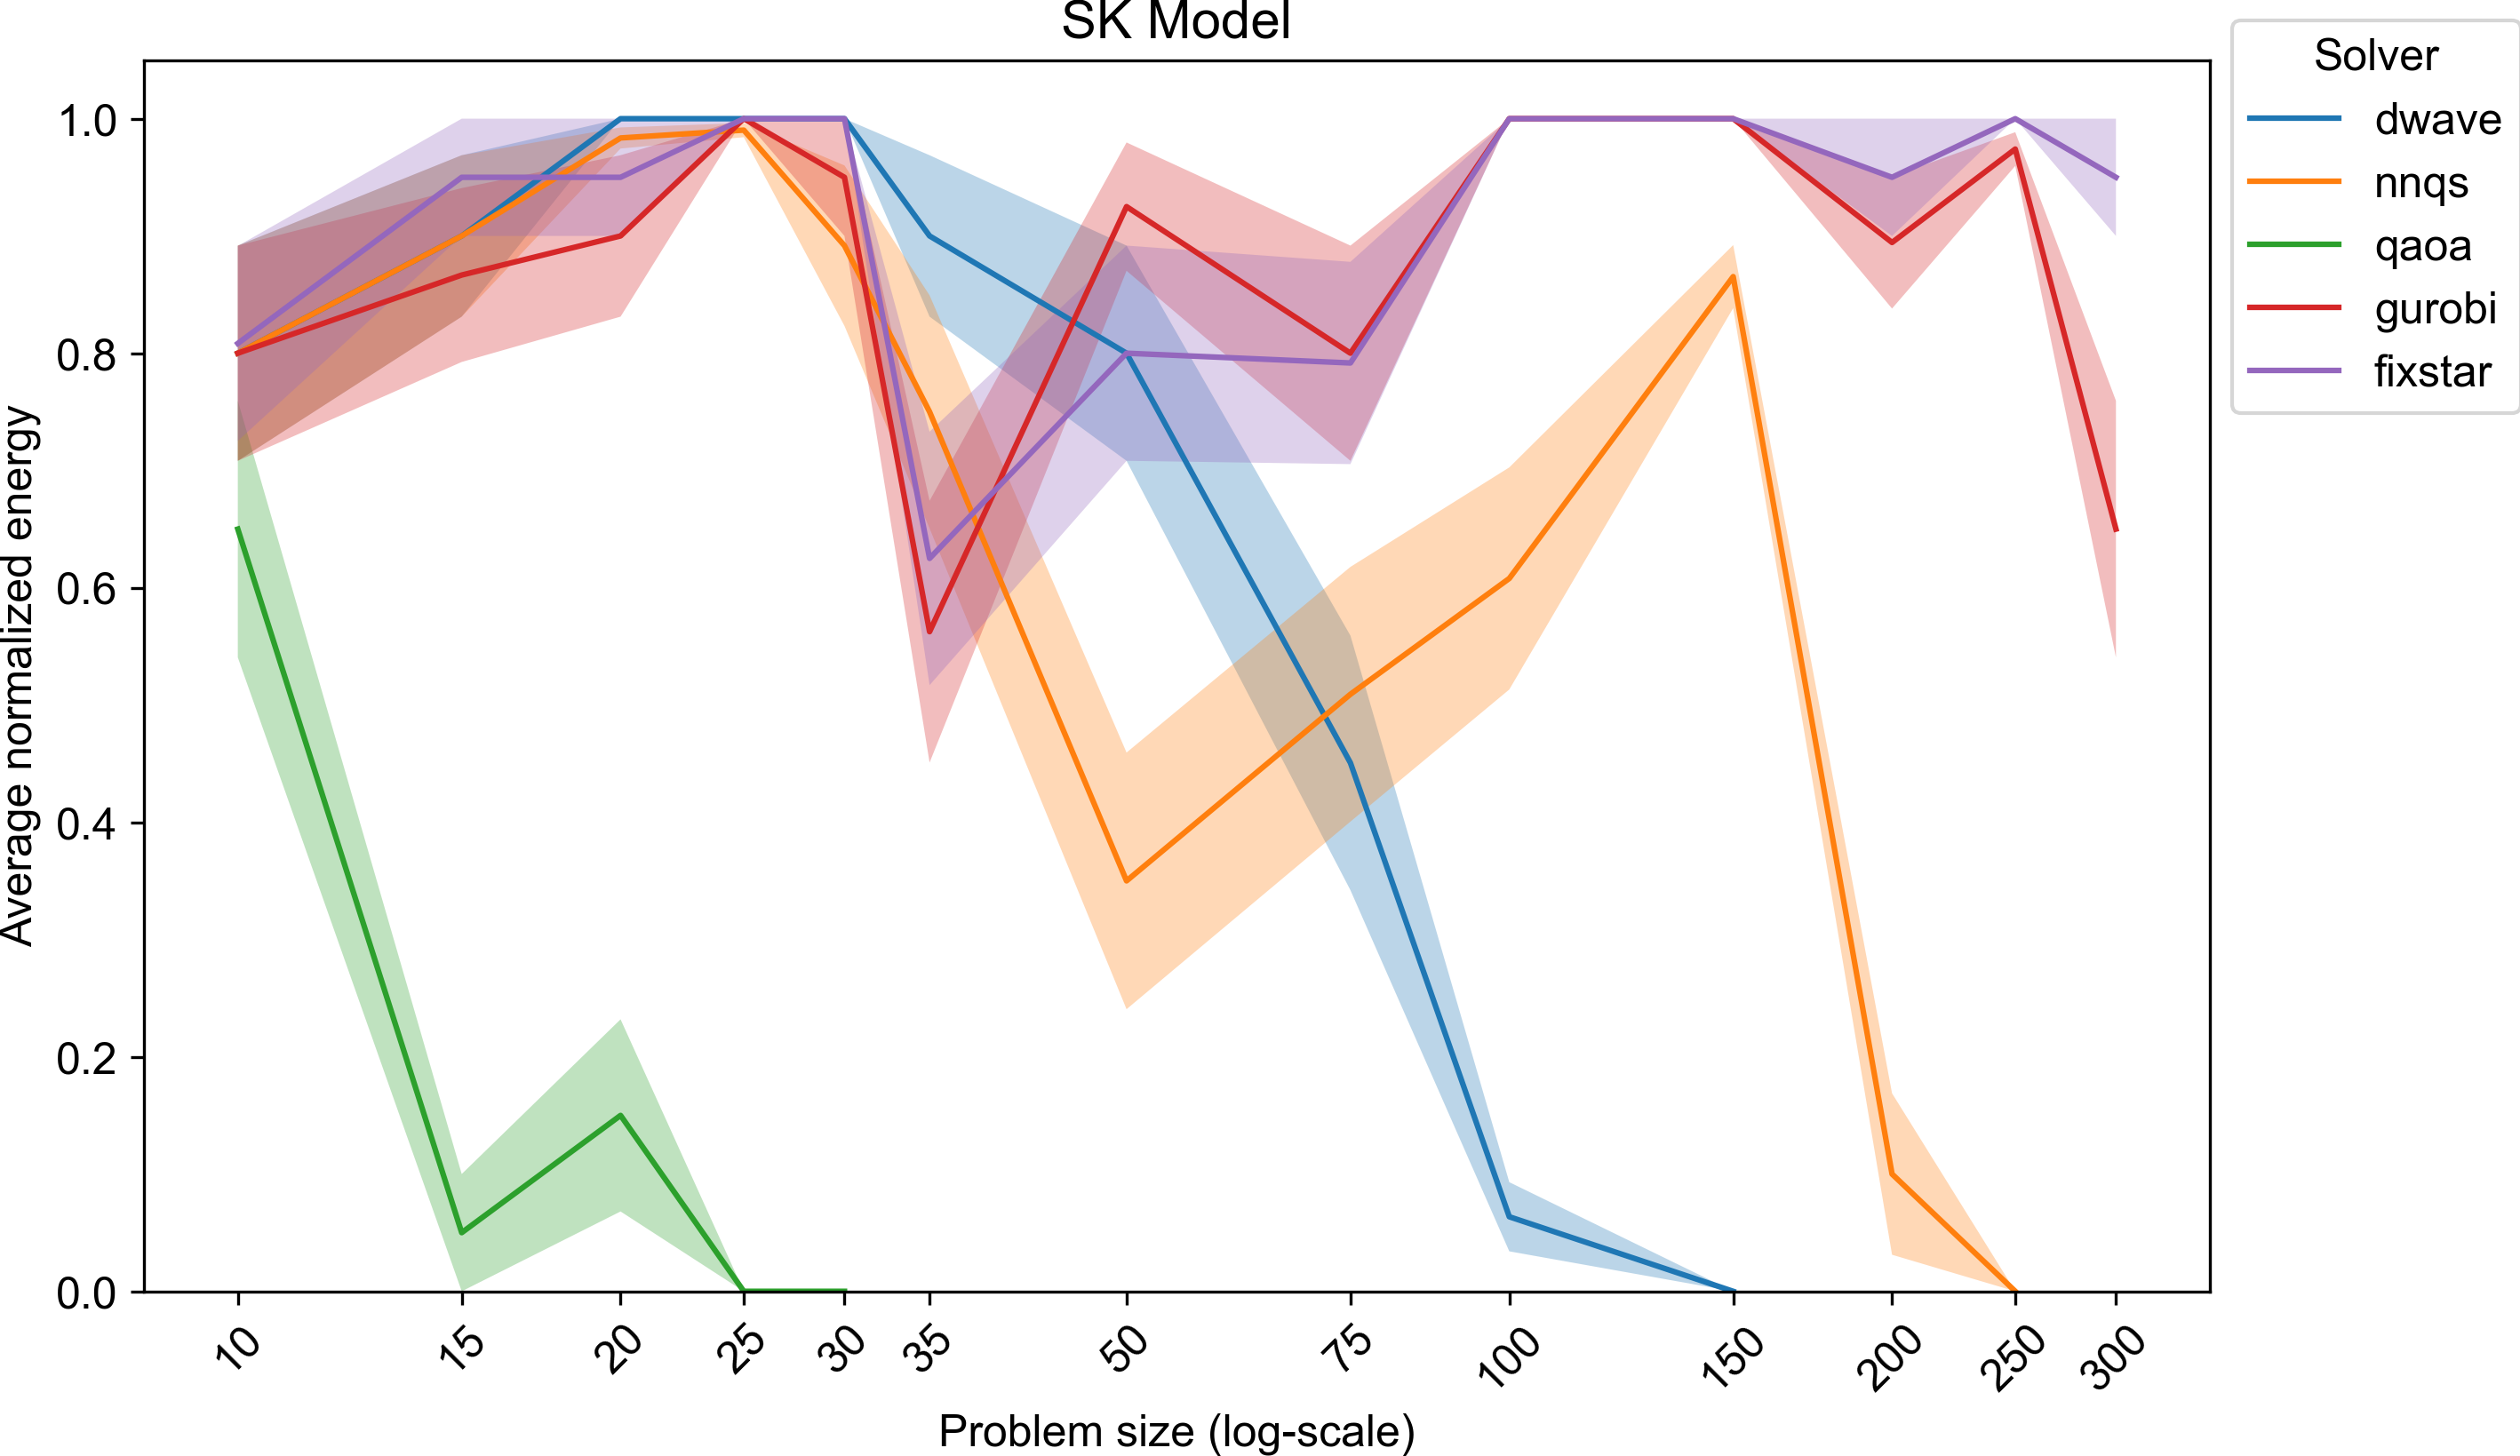
\includegraphics[width=0.9\textwidth]{images/skmodel_all_size.png}}%\hfill
    \\
    \subfloat[Success probability]{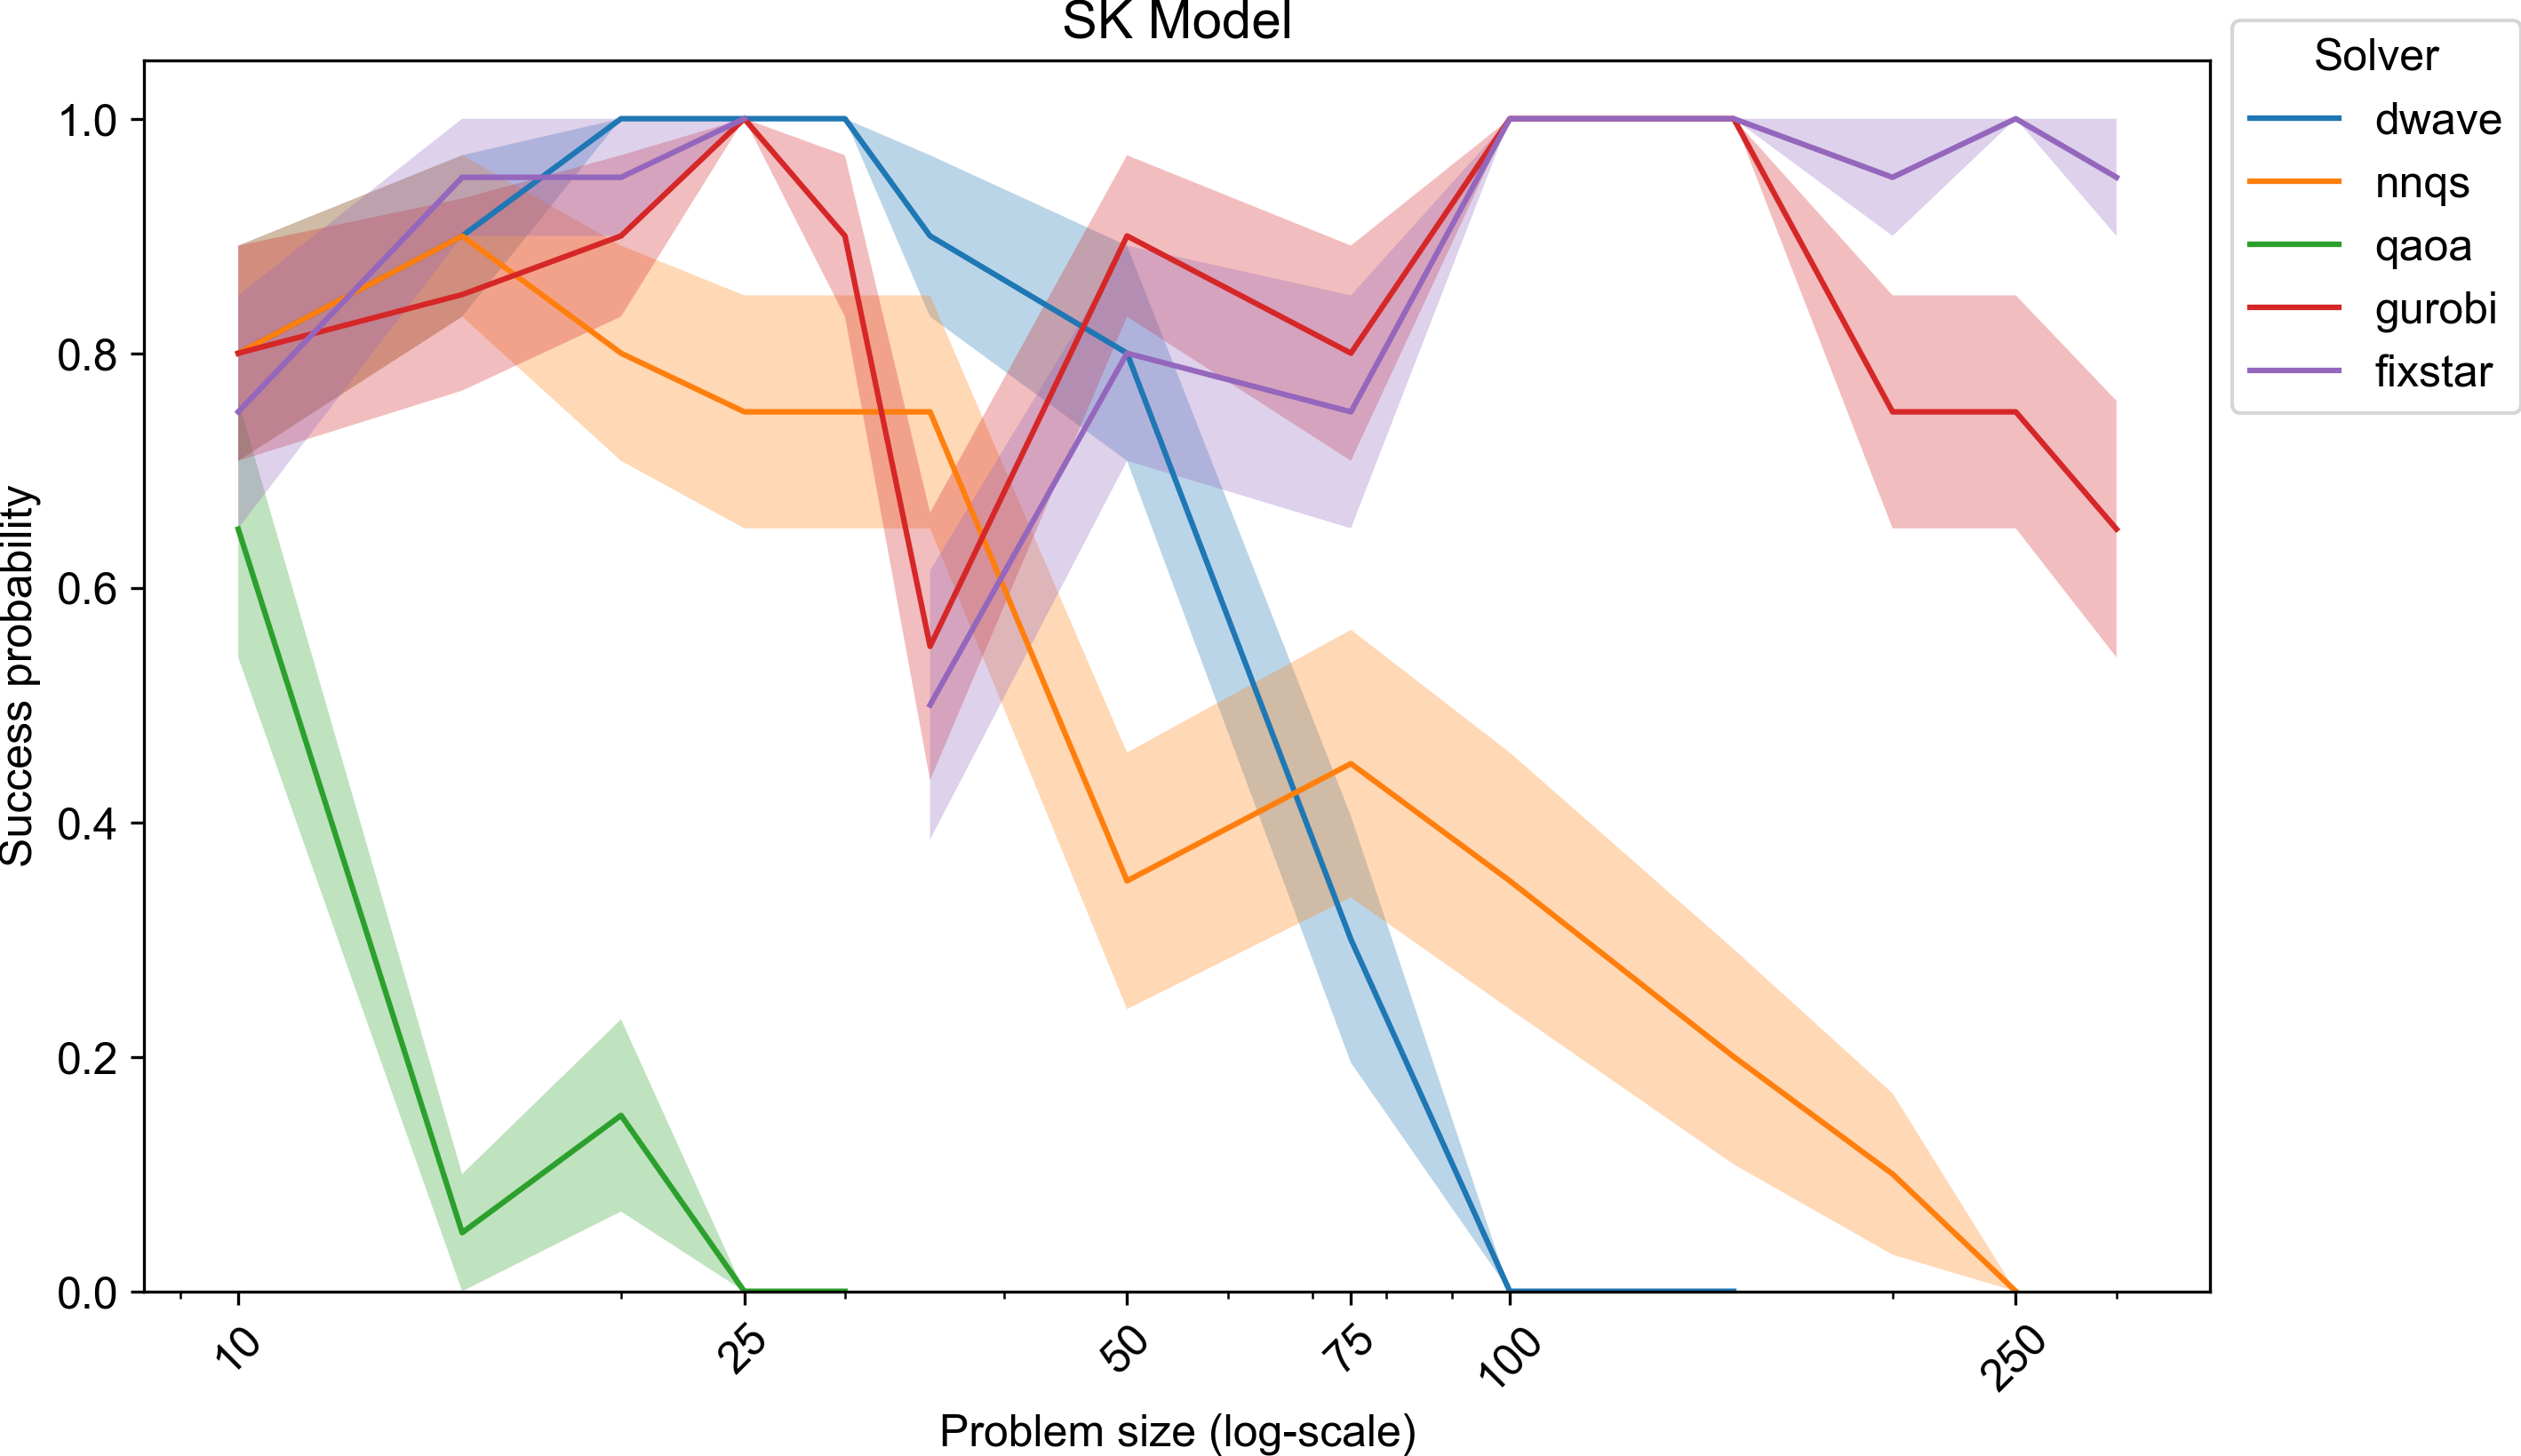
\includegraphics[width=0.9\textwidth]{images/skmodel_all_success_size.png}}
    \caption{Performance of different solvers for SK model by problem size}
    \label{all-skmodel-size}
\end{figure}

\begin{figure}[!htbp]
    \subfloat[Normalized energy]{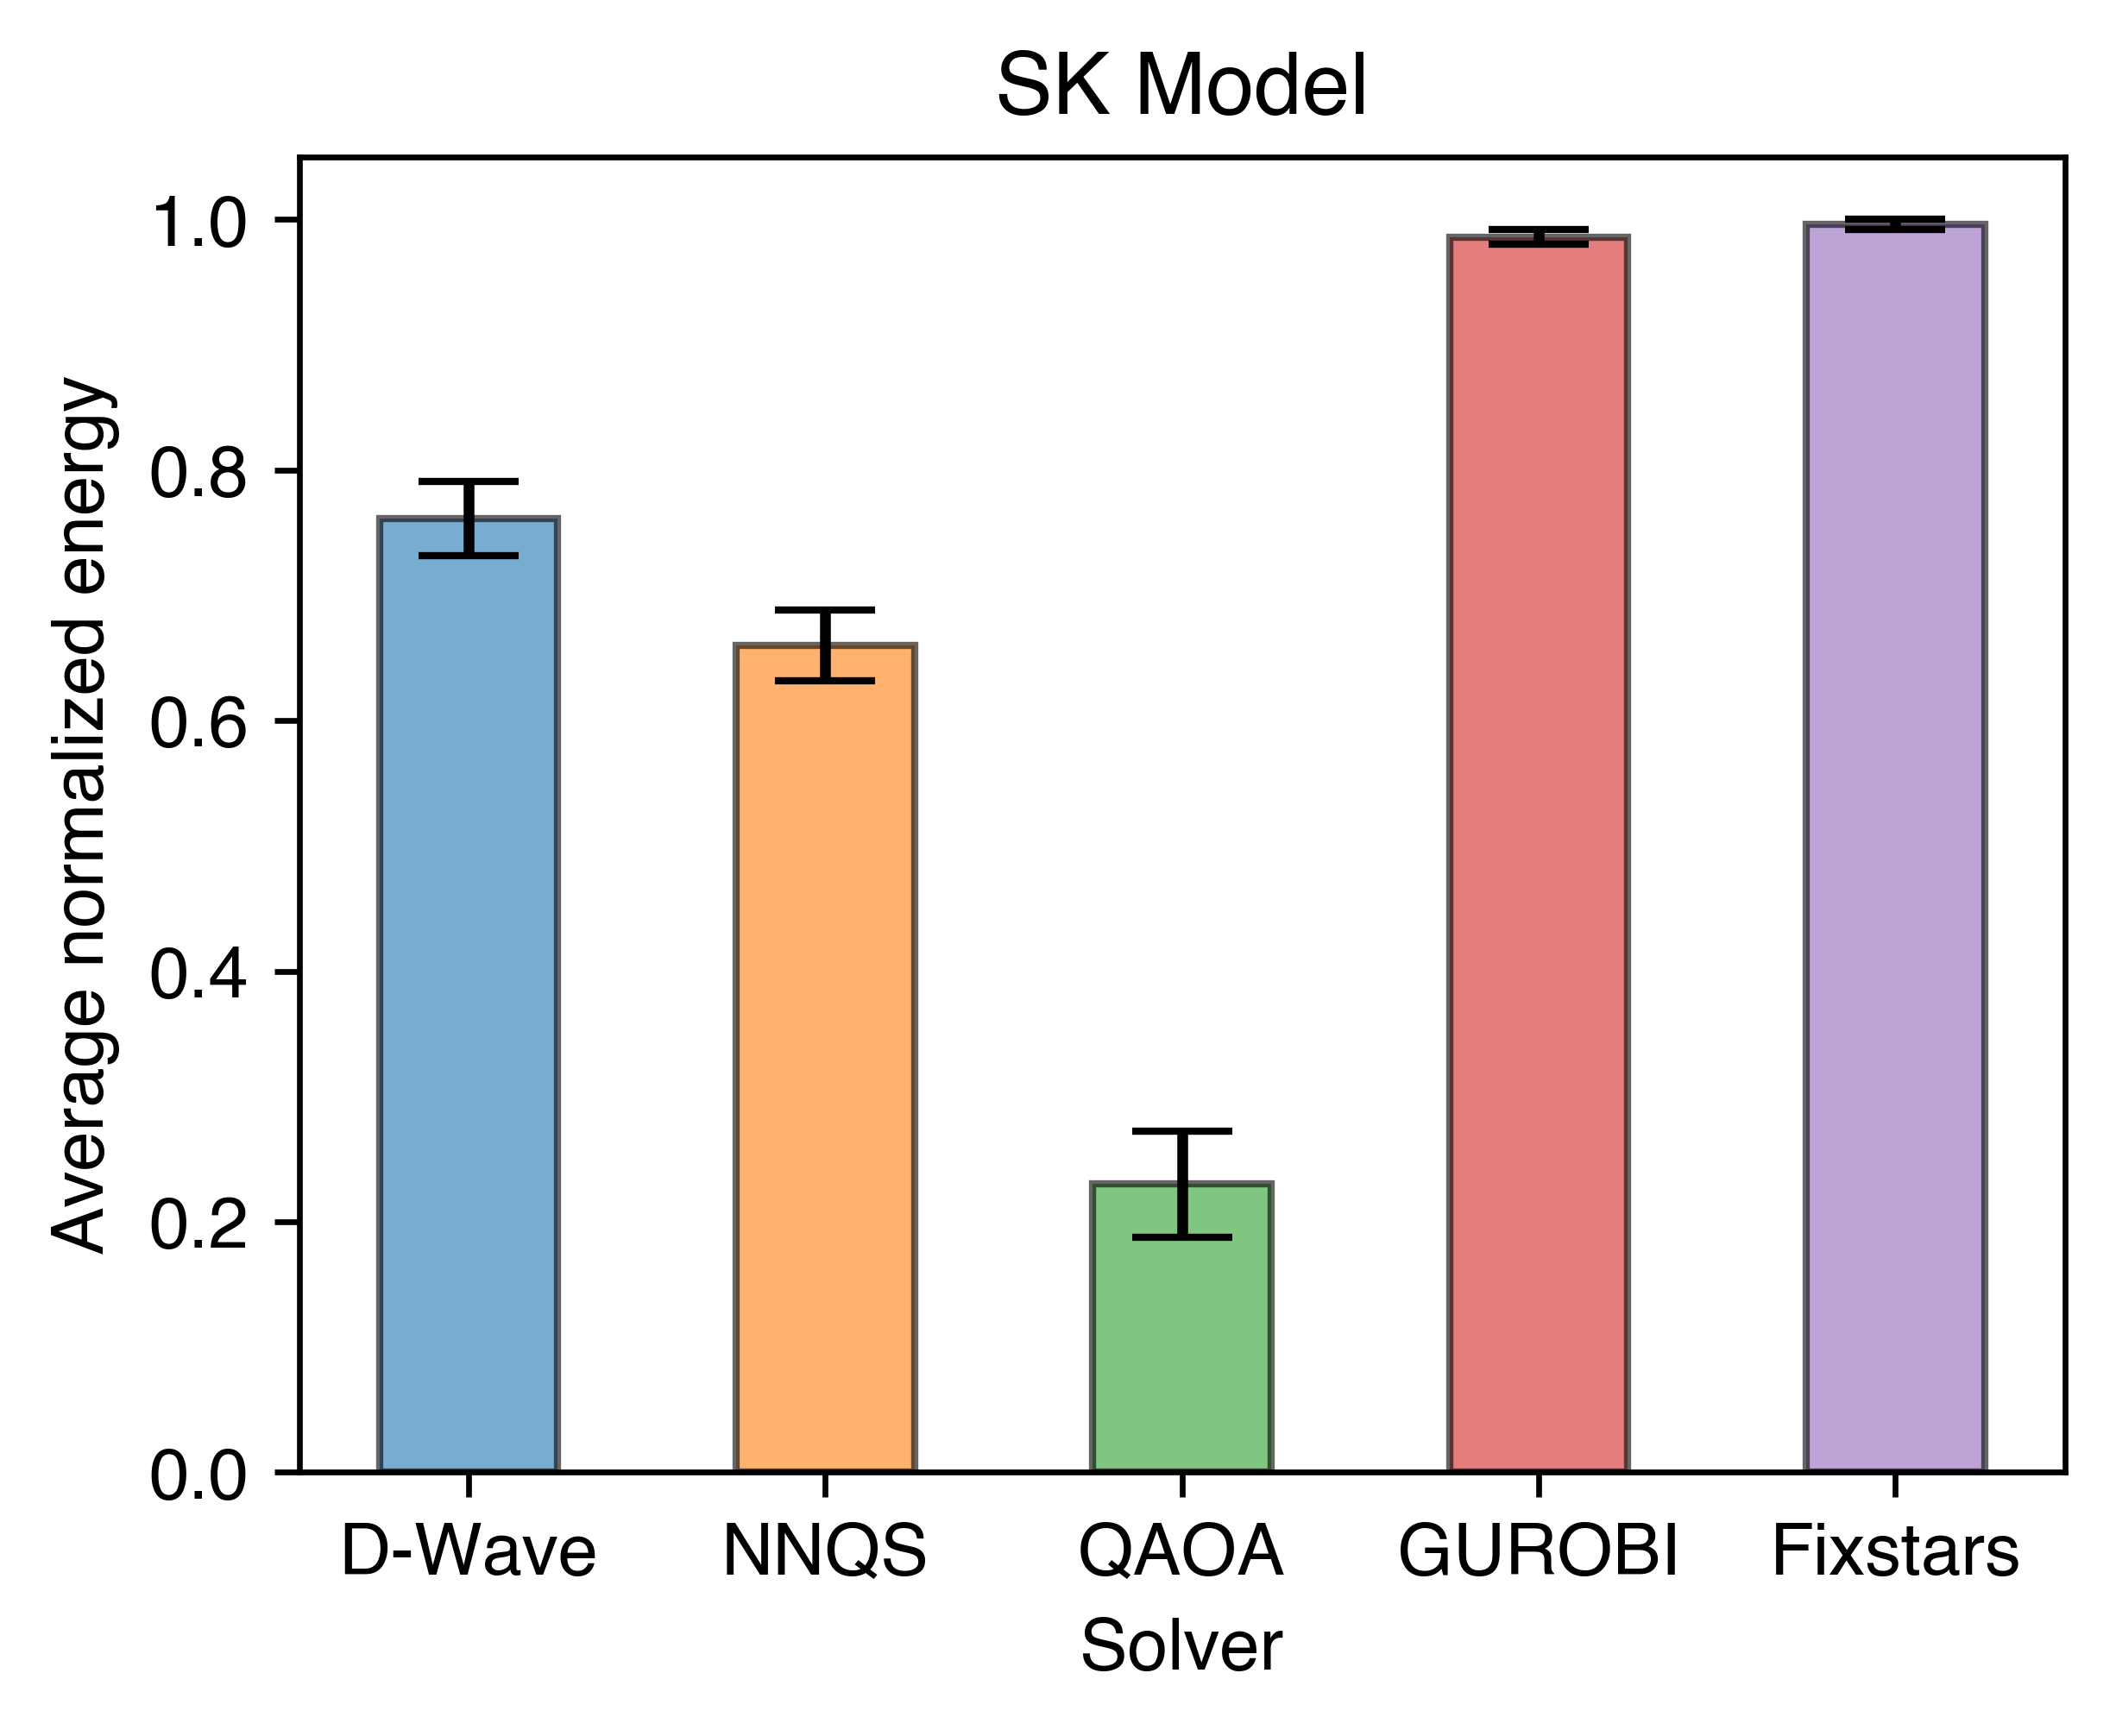
\includegraphics[width=0.49\textwidth]{images/skmodel_all_avg.png}}\hfill
    \subfloat[Success probability]{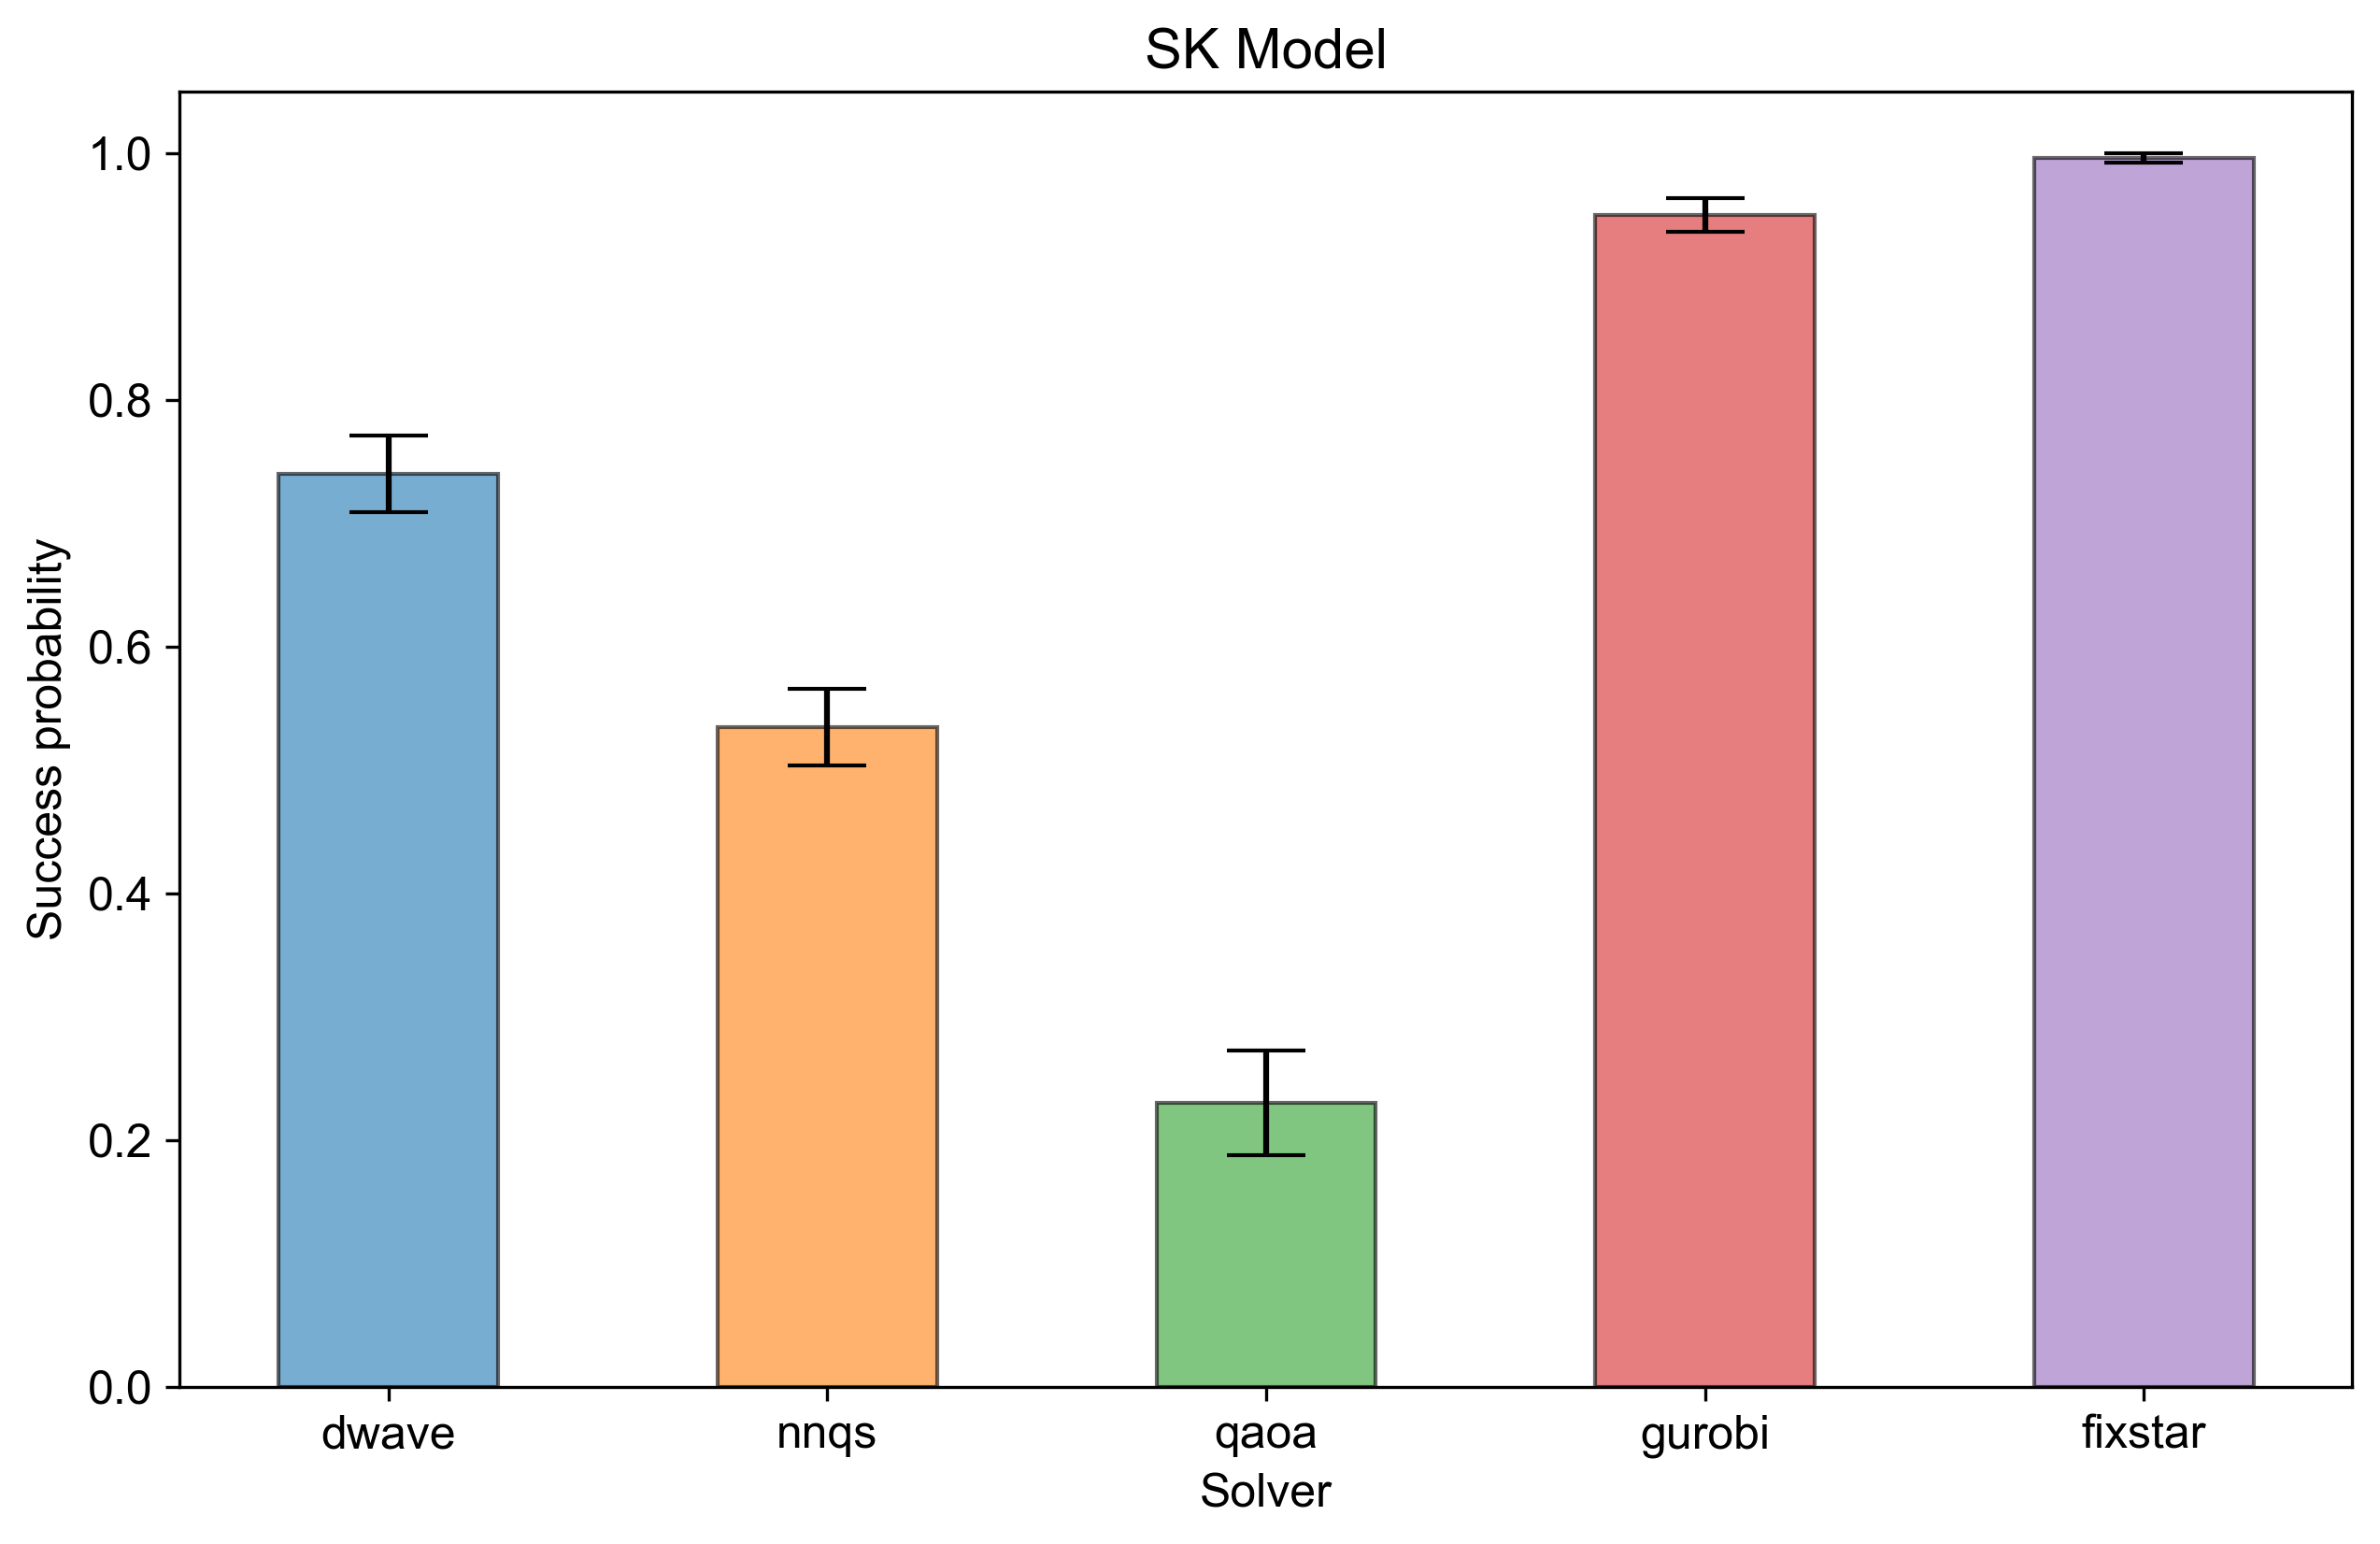
\includegraphics[width=0.49\textwidth]{images/skmodel_all_success_avg.png}}
    \caption{Average performance of different solvers for SK model}
    \label{all-skmodel-average}
\end{figure}

For the SK model dataset, the continuous training algorithm with the RBM generally performed the best in terms of normalized energy and success probability, shown in \autoref{all-skmodel-size}. The performance averaged across all sizes, shown in \autoref{all-skmodel-average}, also highlights that the RBM with a continuous training algorithm performs the best. However, it is interesting that the direct training schemes have poor performance with small problem sizes ($\leq 50$) but are relatively better at higher problem sizes ($100, 250$).

Across all the problem sets, we see that the RBM has a better average performance compared to the MLP in both average normalized energy and success probability for each training algorithm. In terms of training schemes, direct training performs the worst among the 3, and continuous training performs better than progressive training. Using the RBM with a continuous training scheme gives the highest normalized performance across all datasets.

\section{Future Work}
Future studies can explore more QUBO problem types and attempt to classify problems that are difficult for annealing-based solvers such as QA and SA but easier for other solvers such as QAOA.
\chapter{NNQS exploration}\label{nnqsresults}
In this chapter, we will explore the different architectures and training schemes that can be used for training the NNQS to solve QUBO problems. All experiments in this section were run on a subset of the full dataset with problem sizes of $10,25,50,75,200,250$ and $10$ problems for each problem type and size. The problem evaluation metrics are also calculated by considering the solutions from the different types of NNQS to be able to draw a clearer comparison between architectures and training schemes.

\section{Architectures and training schemes}
We will utilize both the Restricted Boltzmann Machine (RBM) and the Multilayer Perceptron (MLP) in their performance as a NNQS. For a given input problem with $n$ variables, the RBM model will have $n$ visible nodes and $5n$ hidden nodes while the MLP will have $n$ input nodes, $1$ hidden layer of size $5n$ and $1$ positive real output node. The RBM uses the sigmoid function while the MLP uses the ReLU activation function. We use Gibbs sampling for the RBM and Metropolis-Hasting sampling for the MLP, both sampling methods are detailed in \autoref{samplingmethods}.

We will also compare 3 training algorithms for NNQS---progressive, direct, and continuous. The progressive training algorithm follows \autoref{alg:progressive}. In direct training, the normalized anneal fraction $s$ is held constant at $1$ for all epochs and follows \autoref{alg:direct}.  In continuous training, the NNQS is not trained to convergence but is trained for a single epoch while incrementing the normalized anneal fraction slowly and follows \autoref{alg:continuous}.

\begin{algorithm}
    \begin{algorithmic}
    \Require Problem Hamiltonian $\hat{H}_c$
    \Ensure Trained NNQS
    \State Initialize NNQS with random weights;
    \State Set $H \leftarrow B(1)\hat{H}_c$;
    \State Train NNQS on $H$ until convergence or until epoch limit of $1000$ is reached;
    \end{algorithmic}
    \caption{NNQS Direct Training}
    \label{alg:direct}
\end{algorithm}

\begin{algorithm}
    \begin{algorithmic}
    \Require Problem Hamiltonian $\hat{H}_c$
    \Ensure Trained NNQS
    \State Initialize NNQS with random weights;
    \For {$s \in [0.001, 1.0]$ step $0.001$}
    \State Set $H(s) \leftarrow A(s)\hat{H}_0 + B(s)\hat{H}_c$;
    \State Train NNQS on $H(s)$ for $1$ epoch;
    \EndFor
    \end{algorithmic}
    \caption{NNQS Direct Training}
    \label{alg:continuous}
\end{algorithm}

The direct training scheme serves as a baseline for directly training a neural network with the cost function as the problem Hamiltonian. The progressive training scheme most closely resembles the quantum annealing process, where the system is kept at the ground state by training until convergence in each increment of $s$. The continuous training scheme is a combination of the other two schemes by slowly incrementing $s$ but never reaching convergence.

\subsection{NAE3SAT}
\begin{figure}[!h]
    \centering
    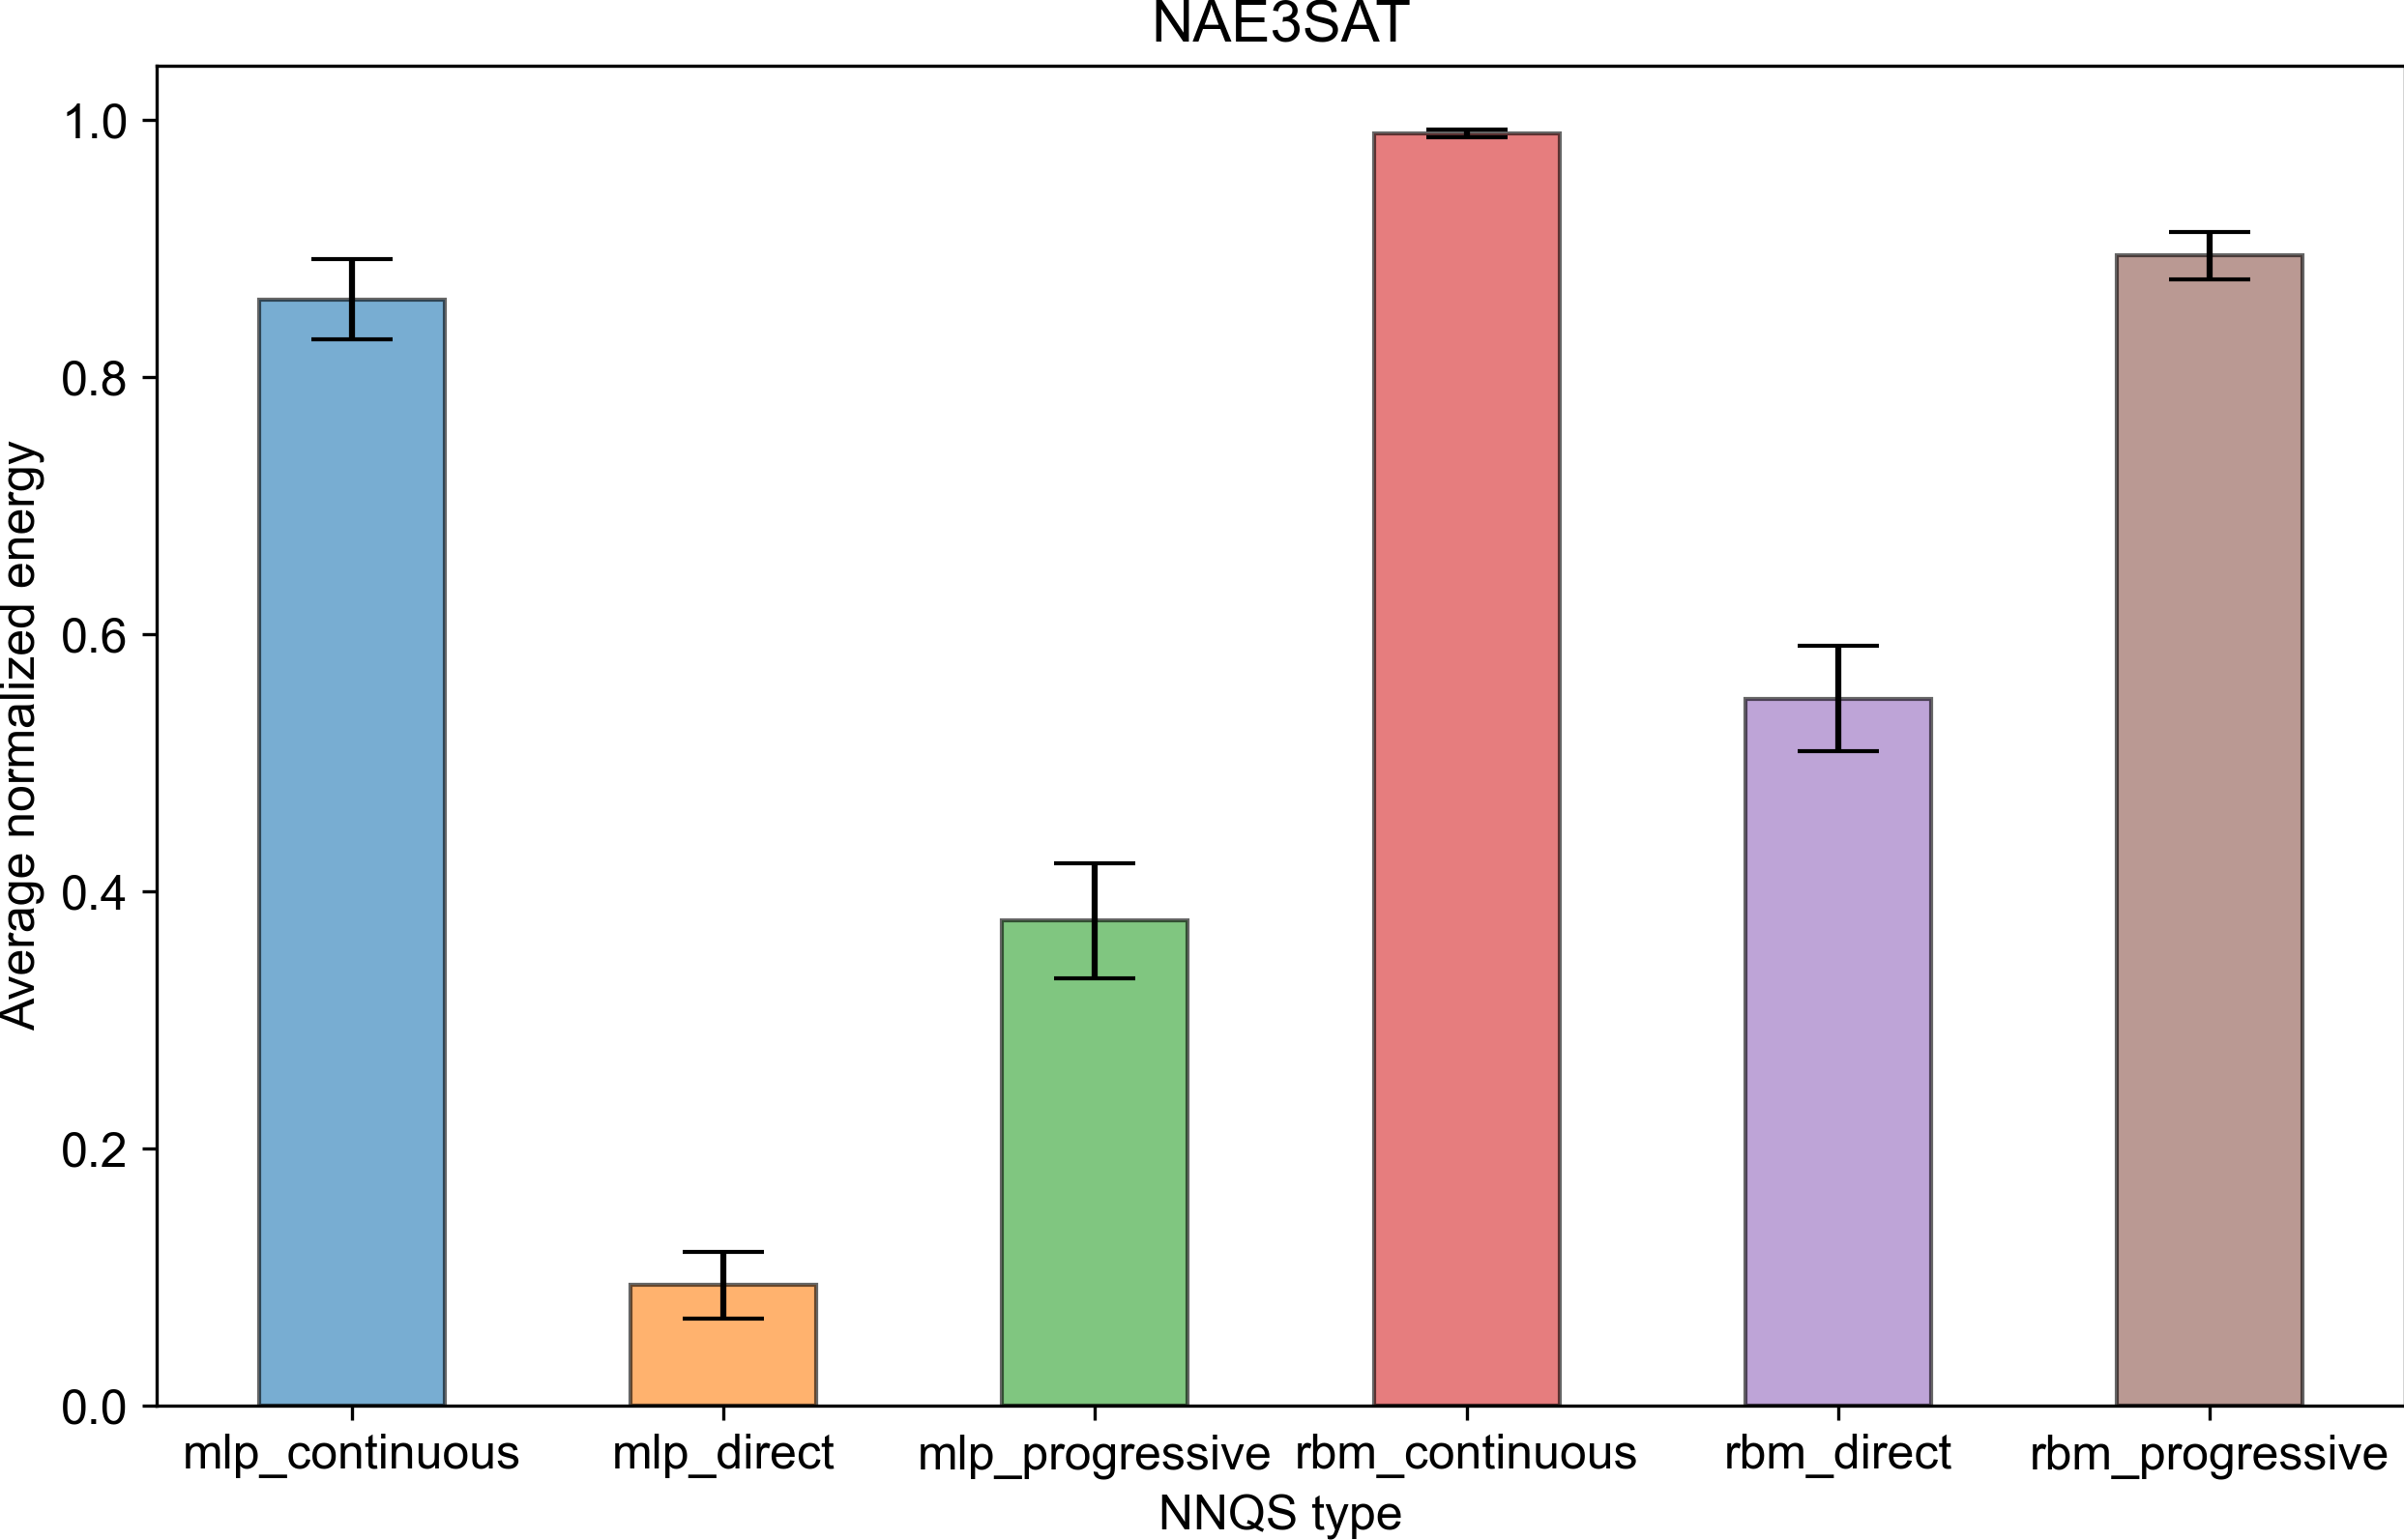
\includegraphics[width=1\linewidth]{images/nae3sat_nnqs_avg.png}
    \caption{Performance of different NNQS types on the NAE3SAT dataset}
    \label{nnqs-nae3sat-average}
\end{figure}

\begin{figure}[!h]
    \centering
    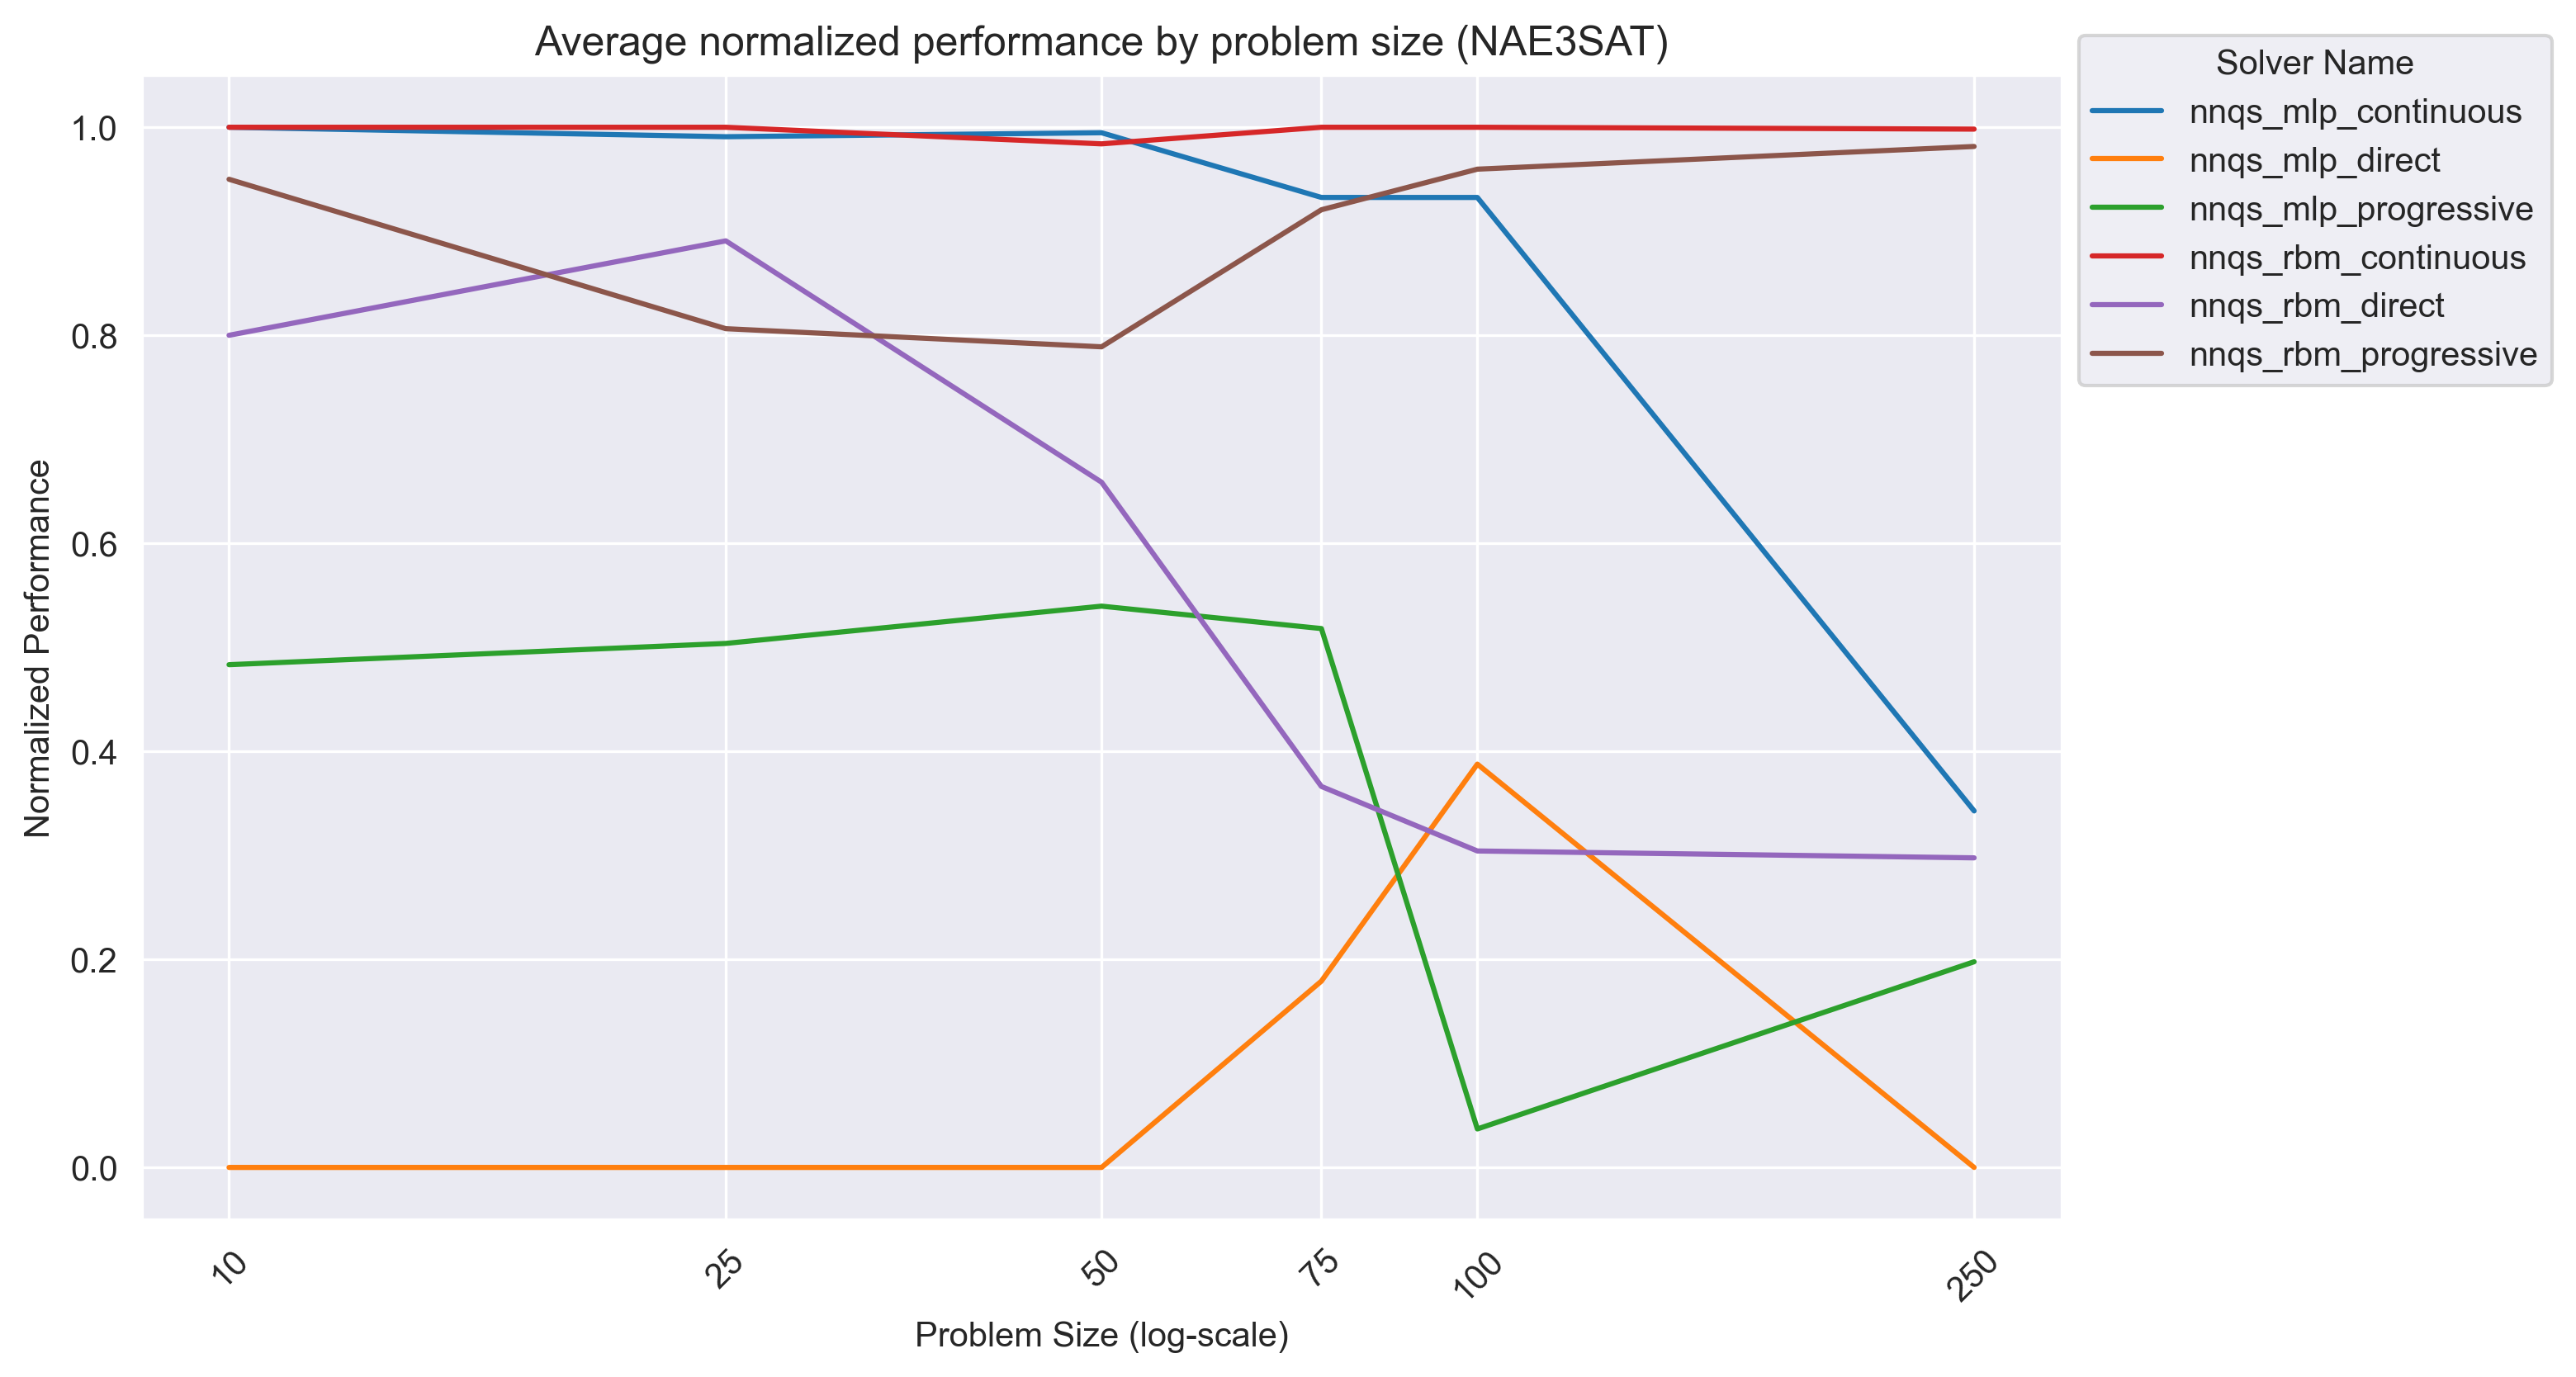
\includegraphics[width=1\linewidth]{images/nae3sat_nnqs_size.png}
    \caption{Performance by size on the NAE3SAT dataset}
    \label{nnqs-nae3sat-size}
\end{figure}

\subsection{Max-cut}
\begin{figure}[!h]
    \centering
    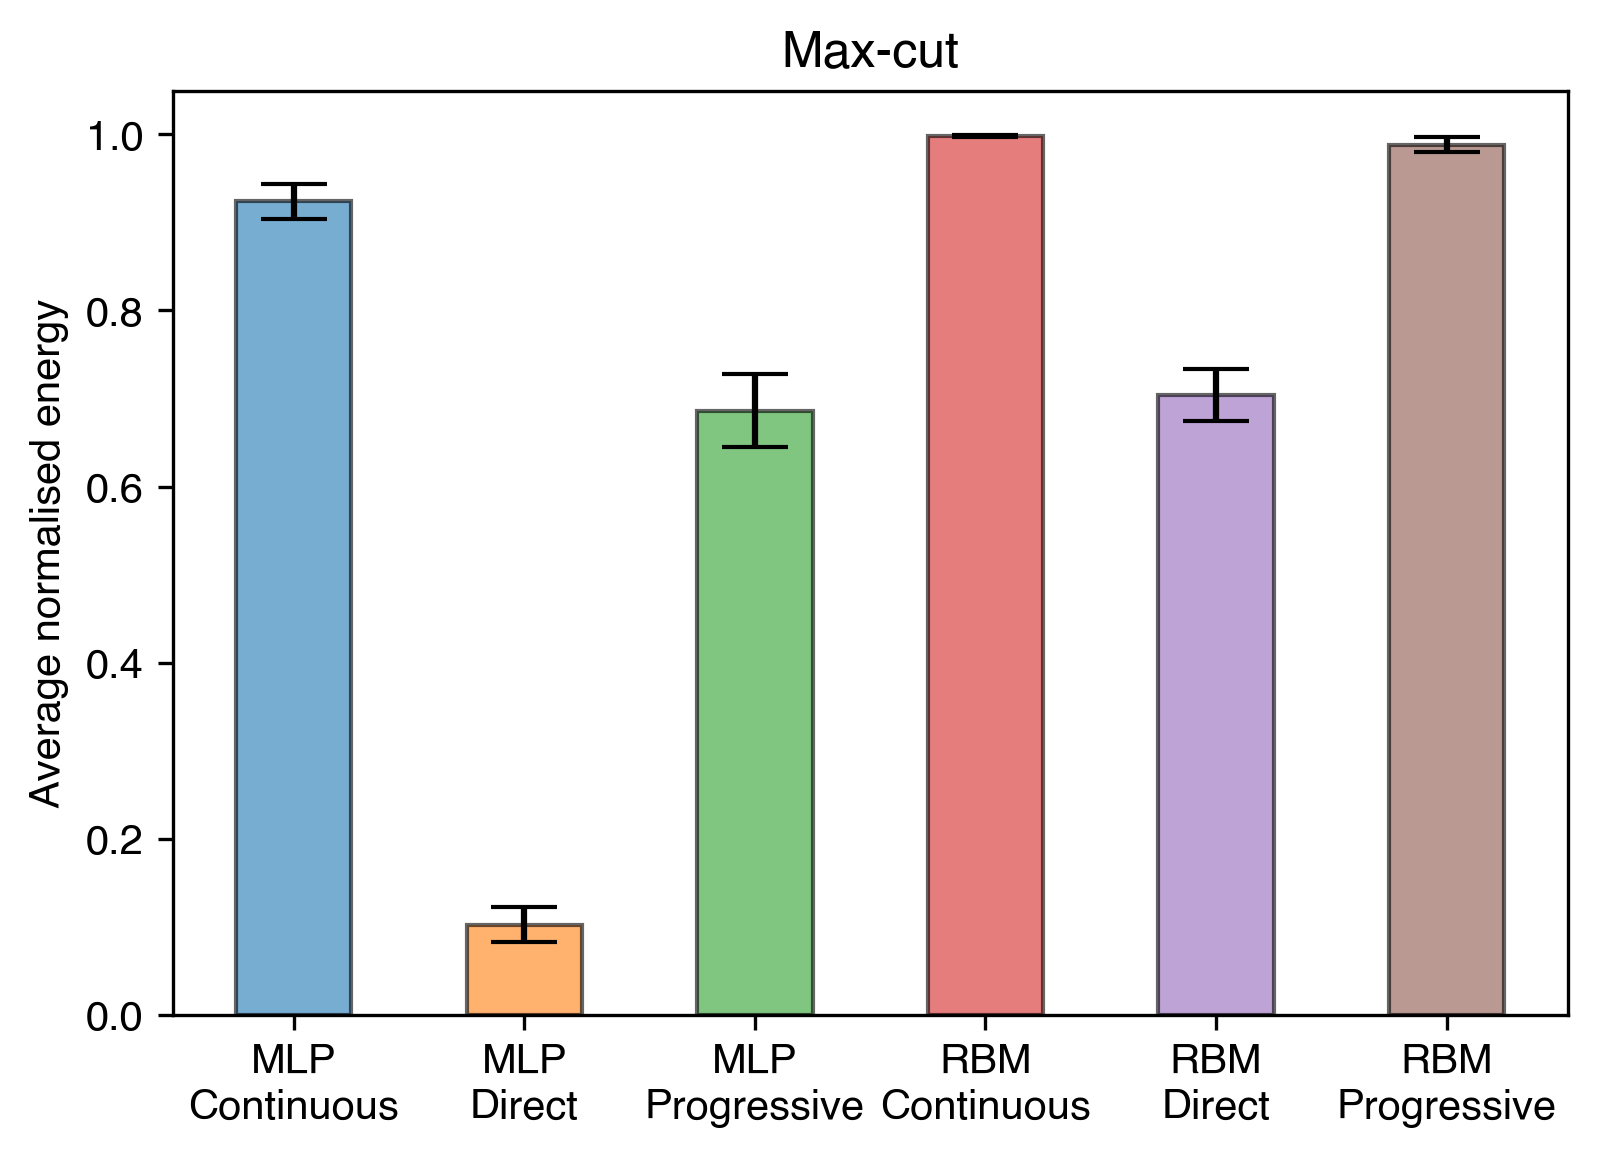
\includegraphics[width=1\linewidth]{images/maxcut_nnqs_avg.png}
    \caption{Performance of different NNQS types on the max-cut dataset}
    \label{nnqs-maxcut-average}
\end{figure}

\begin{figure}[!h]
    \centering
    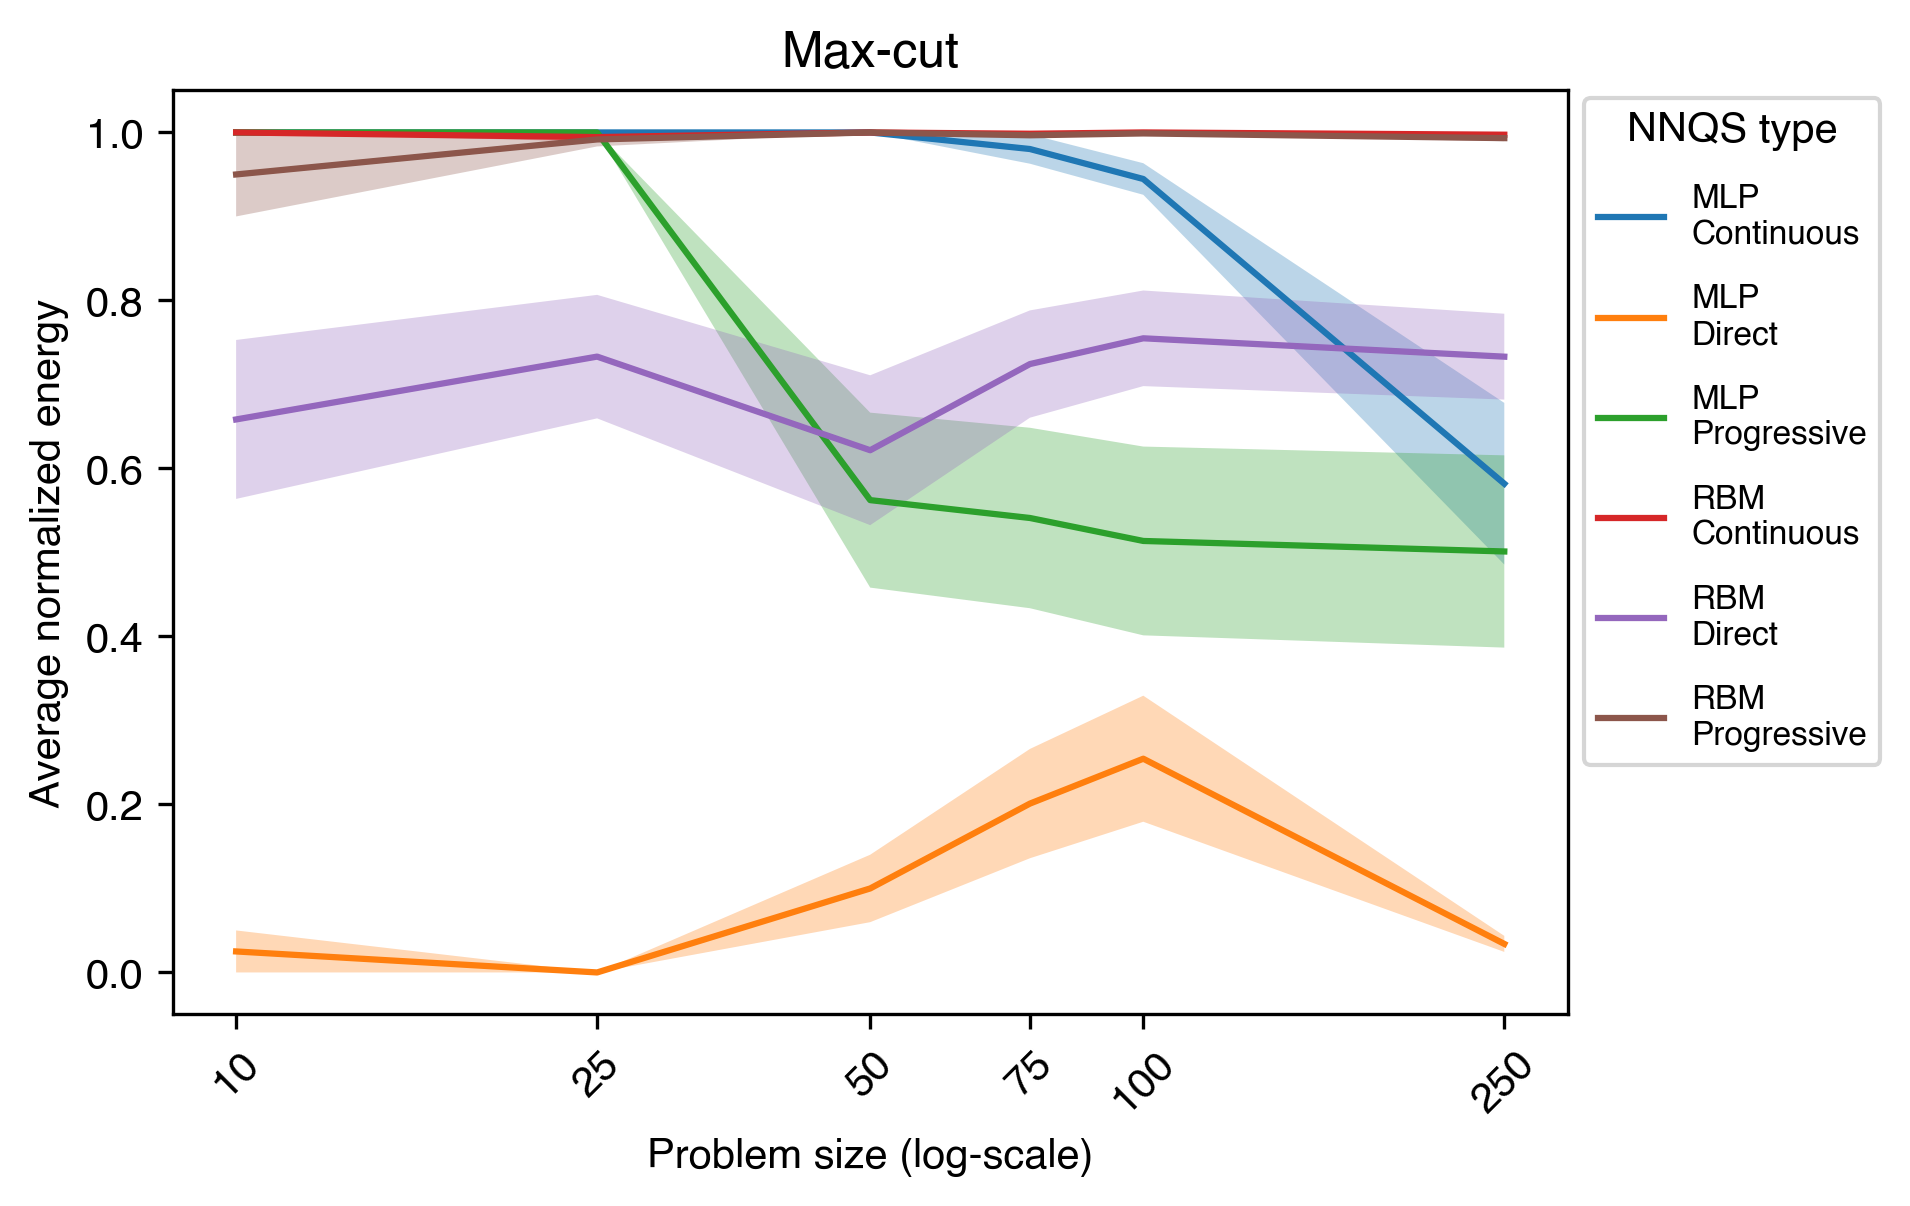
\includegraphics[width=1\linewidth]{images/maxcut_nnqs_size.png}
    \caption{Performance by size on the max-cut dataset}
    \label{nnqs-maxcut-size}
\end{figure}

\subsection{SK Model}
\begin{figure}[!h]
    \centering
    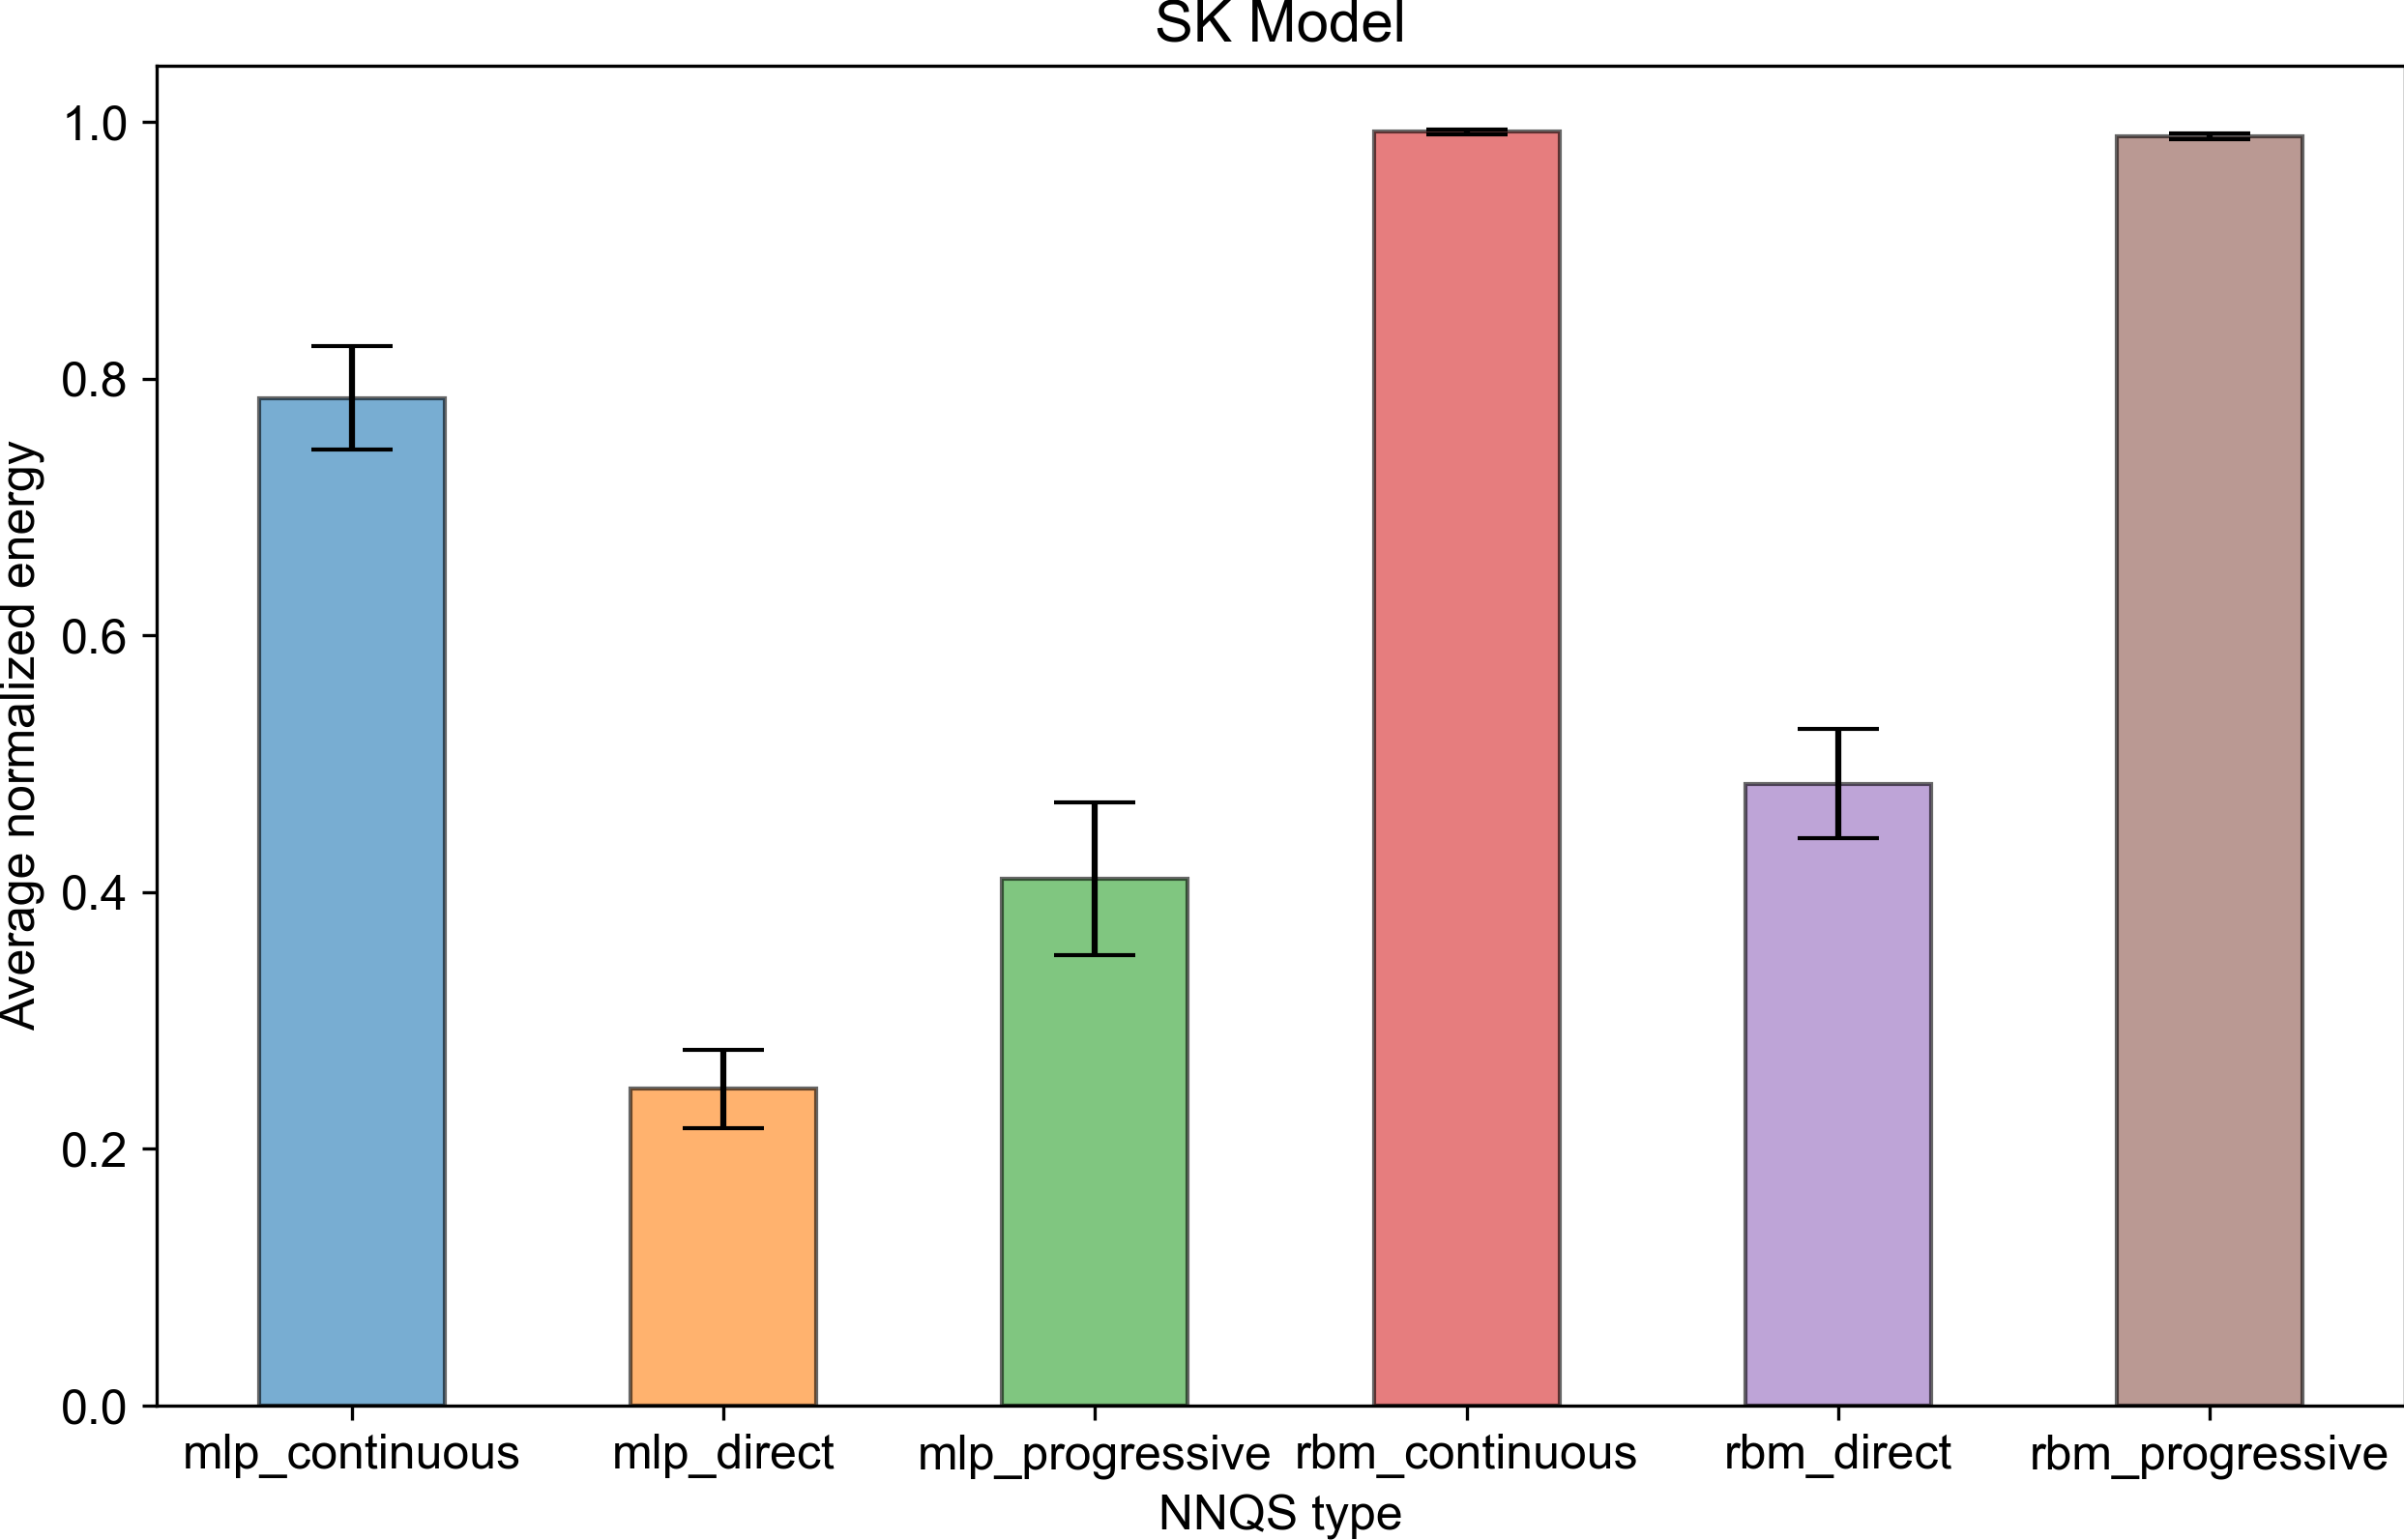
\includegraphics[width=1\linewidth]{images/skmodel_nnqs_avg.png}
    \caption{Performance of different NNQS types on the SK model dataset}
    \label{nnqs-skmodel-average}
\end{figure}

\begin{figure}[!h]
    \centering
    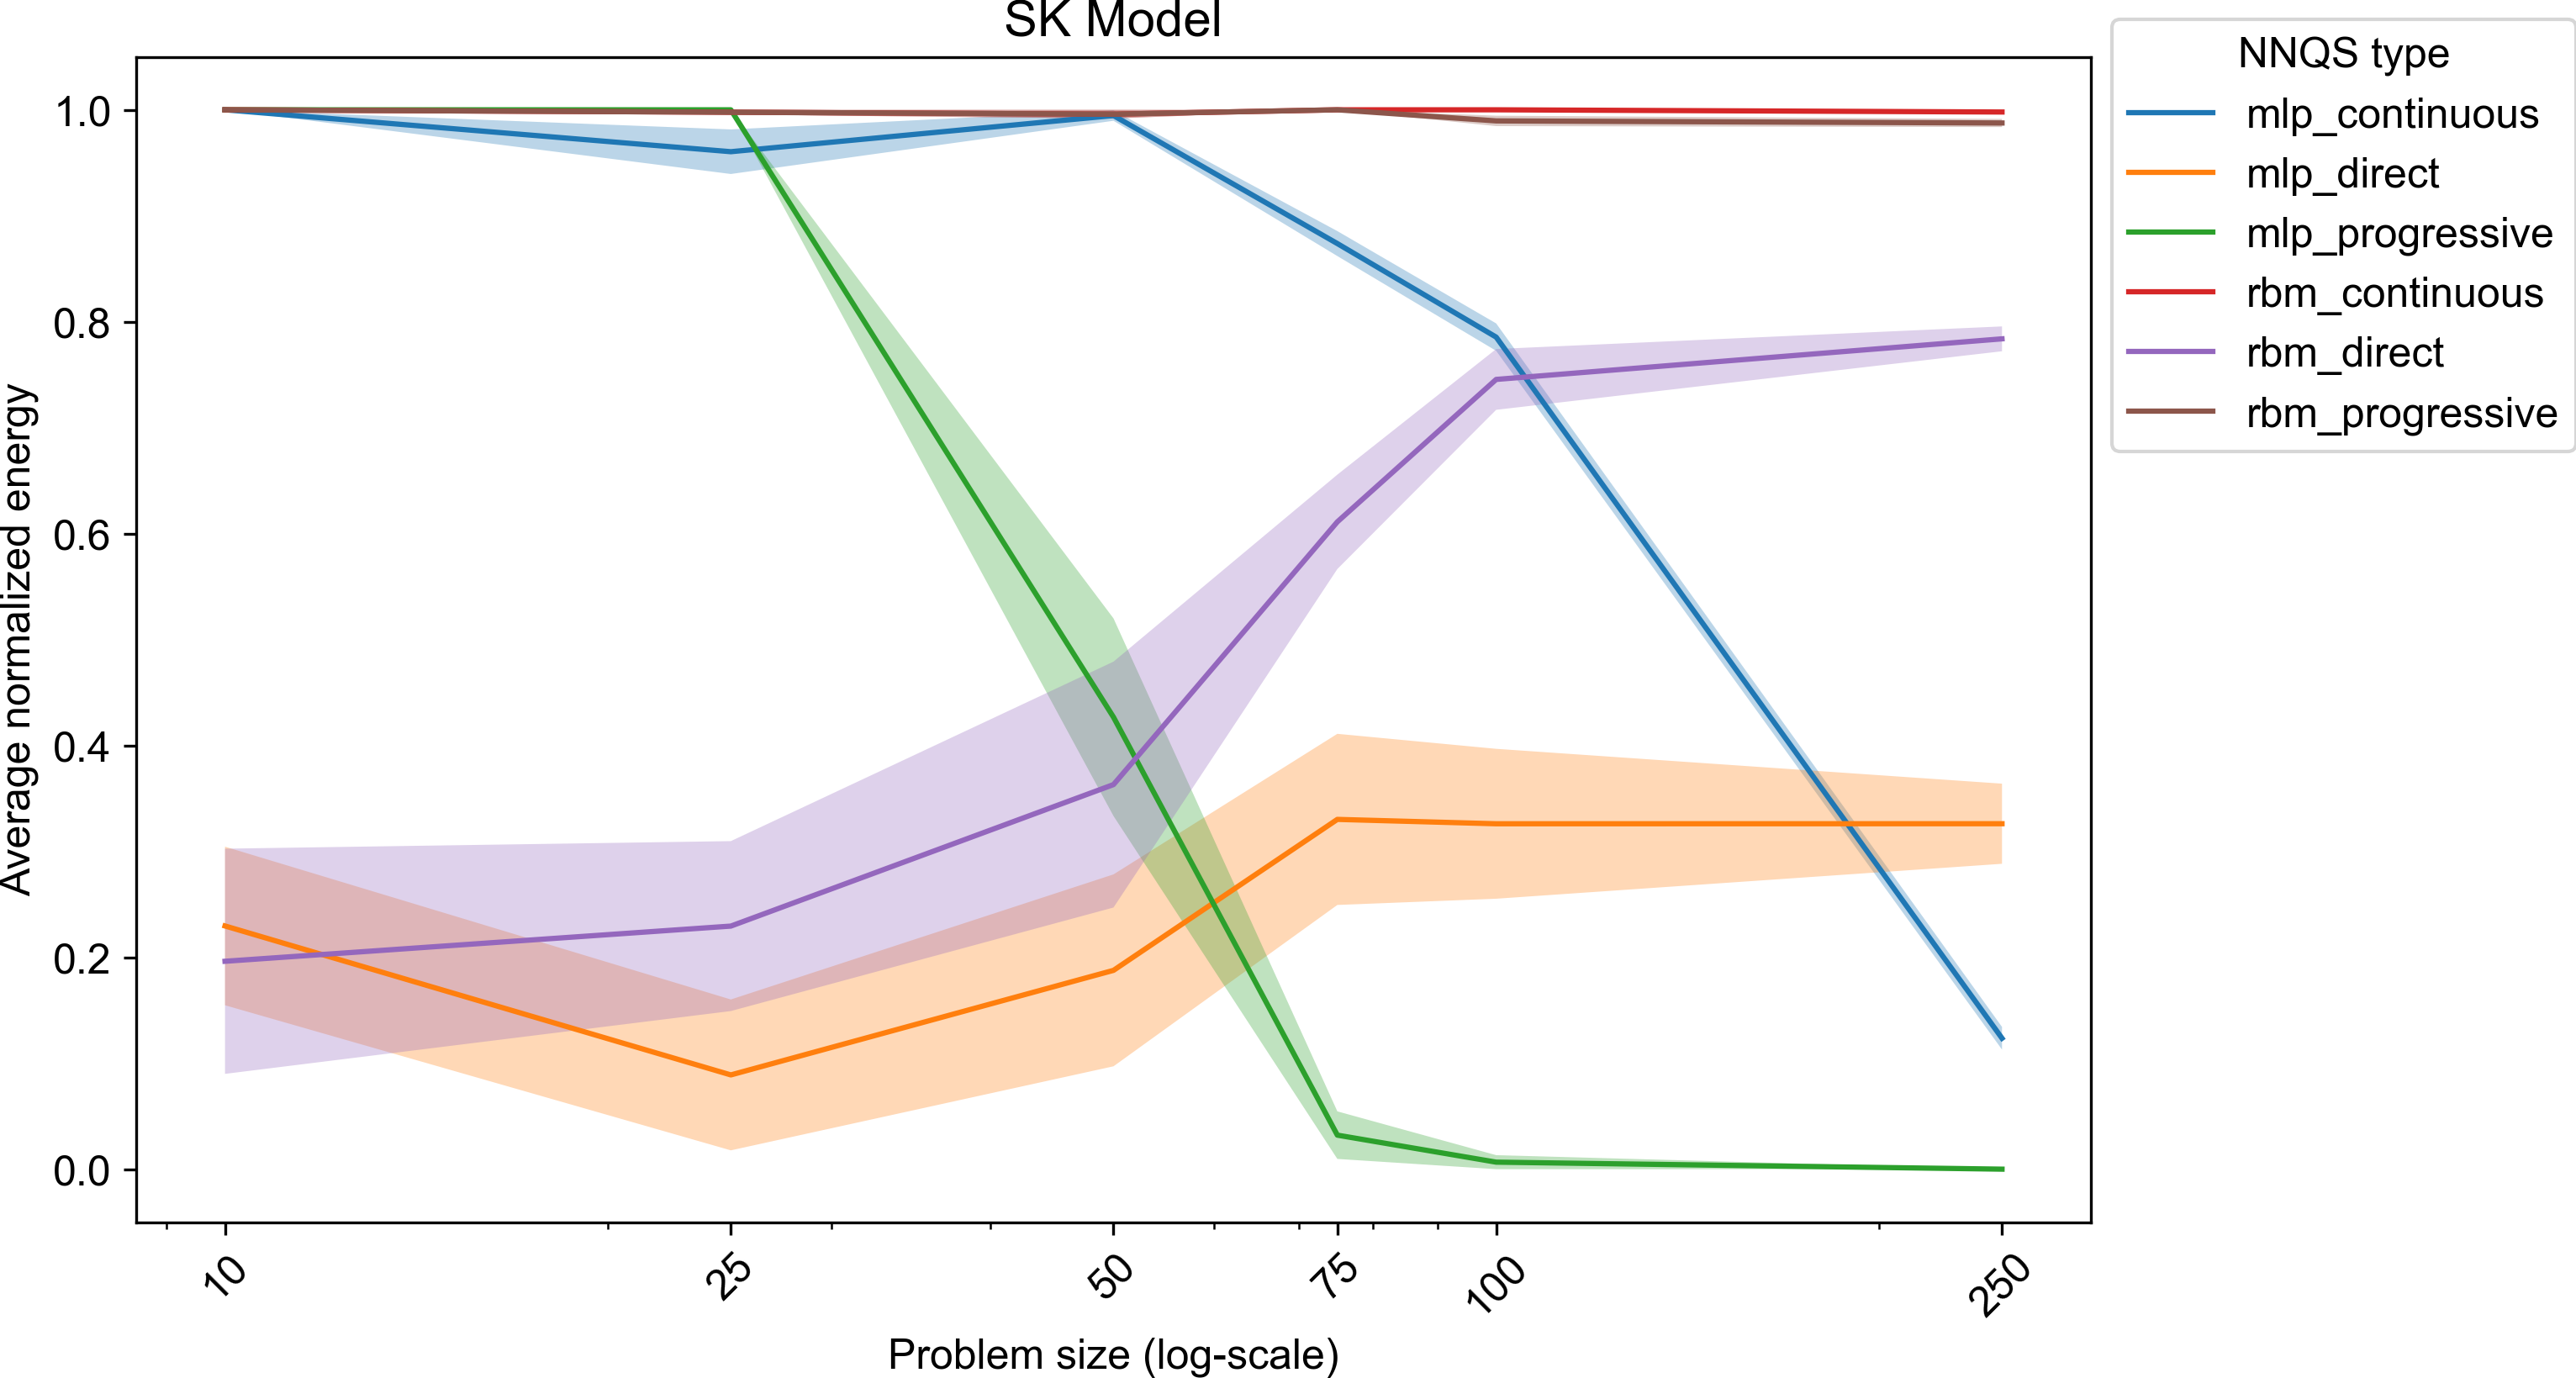
\includegraphics[width=1\linewidth]{images/skmodel_nnqs_size.png}
    \caption{Performance by size on the SK model dataset}
    \label{nnqs-skmodel-size}
\end{figure}

Using the RBM with a continuous training scheme gives the highest normalized performance across all datasets.

\section{Future Work}
Future studies could investigate if more state-of-the-art machine learning models such as Graph Neural Networks or Attention-based Neural Networks can be used as the underlying architecture for NNQS.

To investigate whether the NNQS closely models the wave function of a D-wave solver in the annealing process, we can do a quench of the D-wave annealing process in order to take a snapshot of the intermediate state. Some initial work is detailed in \autoref{appendix:quenching} but is not included in the main report as the results are not substantial.
\chapter{Conclusion}

This chapter summarises our study's contributions and limitations. It also makes recommendations for further work that future projects could investigate.

\section{Contributions}
In this study, we have benchmarked $5$ QUBO solvers:
\begin{enumerate}
    \item D-Wave Quantum Annealer
    \item Neural Network Quantum States (NNQS)
    \item Quantum Approximate Optimization Algorithm (QAOA)
    \item GUROBI Optimizer
    \item Fixstars Amplify QUBO Solver
\end{enumerate}
We used three types of combinatorial optimisation problems: not-all-equal 3-satisfiability (NAE3SAT), max-cut, and Sherrington-Kirkpatrick model (SK model) problems as datasets to evaluate the solvers' performance.

Our results show that the D-Wave and NNQS solvers perform the best among the quantum-inspired solvers. The NNQS solver is generally better than the D-Wave solver except for the SK model dataset. The QAOA solver achieves generally poor performance across datasets and is not comparable due to the limitations on problem size. All three quantum-inspired solvers underperform the two classical solvers, with the simulated-annealing-based Fixstars solver achieving the best performance for all datasets.

When the runtimes of the D-Wave, GUROBI, and Fixstars solvers were matched, the D-Wave solver could outperform the GUROBI solver for specific ranges of problem sizes. This inspires further development of quantum annealers that can handle larger problems with dense connectivity.

We also investigated the NNQS solver with different architectures and training algorithms. The Restricted Boltzmann Machine (RBM) and the Multilayer Perceptron (MLP) were used as the underlying neural networks along with three different training algorithms---progressive, direct, and continuous. We found that the RBM with a continuous training scheme performs best across all datasets.

\section{Limitations and Future Work}
The primary constraint of our study came from the limitations of the QAOA solver, which was intended to be run on a gate-based quantum computer. Due to restricted availability of real quantum computers, we used a quantum simulator capable of handling only up to $30$ variables. Nevertheless, as the simulator does not model quantum noise and the results from the QAOA solver for small problems are not promising, QAOA on an real quantum computer would likely perform even worse for larger problems and is thus not too interesting to benchmark in the current NISQ era. Another limitation was that there were many parameters for each solver that we did not have the resources to optimise for, such as the annealing time for the D-Wave solver and various forms of the QAOA Ansatz. These might be more suitable for future projects that investigates one specific QUBO solver.

Future studies can explore more QUBO problem types and attempt to classify problems that are difficult for annealing-based solvers, such as quantum annealers and simulated annealers, but easier for other solvers like the QAOA solver. When gate-based quantum computers are readily available, the QAOA solver with larger $p$ values ($p > 1$) could also be benchmarked, which has been shown to perform better but requires more computational resources.

For further work with NNQS, future studies could investigate if more modern machine learning models, such as Graph Neural Networks or Attention-based Neural Networks, can be used as the underlying architecture for NNQS and whether they provide better performance. It would also be interesting to investigate why the continuous training scheme performs better than the progressive training scheme.

Future studies could also determine whether NNQS closely approximates the wave function of a D-Wave solver during the quantum annealing process. A quench of the D-Wave annealing process can help take a snapshot of the intermediate state, which can be compared to the intermediate sampling results from the NNQS solver. Extra information is included in \autoref{appendix:quenching}.

\bibliographystyle{socreport}
\bibliography{report}

% Appendix (Remove if no appendix)
\appendix
\chapter{Reformulating the knapsack problem as a QUBO problem}\label{appendix:knapsack}

This appendix explains an example of how a combinatorial optimisation problem with inequality constraints can be formalised as a QUBO problem. The knapsack problem is a classic combinatorial optimisation problem with a knapsack with integer weight limit $W > 0$ and $n$ items, each with a weight $w_i > 0$ and profit $c_i > 0$. The problem seeks to find the optimal set of items to place in the knapsack to maximise total profit while not exceeding the weight limit. Formally, we have
\begin{align}
\max &\sum_{i=1}^n c_i x_i \label{eq:knapsack_cost}\\
\mathrm{st.} &\sum_{i=1}^n w_i x_i \leq W \label{eq:knapsack_constraint}\\
x_i &\in \{0,1\}^n \nonumber
\end{align}
The quantity \refeq{eq:knapsack_cost} refers to the total profit of the chosen items, and constraint \refeq{eq:knapsack_constraint} keeps the total weight below the weight limit. To convert this optimisation problem into a QUBO problem, we can include the inequality constraint in our QUBO formulation by introducing slack variables, $y_j$'s, which turn the inequality constraint into an equality constraint~\cite{b6}.
\begin{align}
\max &\sum_{i=1}^n c_i x_i \\
\mathrm{st.} &\sum_{i=1}^n w_i x_i = \sum_{j=1}^W jy_j \label{eq:knapsack_slack_weight}\\
&\sum_{j=1}^W y_j = 1 \label{eq:knapsack_slack_sum}\\
x &\in \{0,1\}^n, y \in \{0,1\}^W \nonumber
\end{align}
The slack variables $y_j$ track the total weight of the knapsack with $y_j = 1 \Leftrightarrow$ total weight is $j$. Constraint \refeq{eq:knapsack_slack_sum} ensures that only one of $y_j$ equals $1$. With penalty parameters $C_1 > \sum_{i=1}^n c_i$ and $C_2 > \sum_{i=0}^n c_i$, we can formulate the following QUBO problem:
\begin{align}
    \max f(x, y) &\coloneqq \sum_{i=1}^n c_i x_i - C_1 P_w^2 - C_2 P_n^2 \\
    P_w &\coloneqq \sum_{i=1}^n w_i x_i - \sum_{j=1}^W jy_j \\
    P_n &\coloneqq 1 - \sum_{j=1}^W y_j \\
    x &\in \{0,1\}^n, y \in \{0,1\}^W \nonumber
\end{align}
Since the penalty parameters are larger than $\sum_{i=1}^n c_i$, the optimal solution to the QUBO problem must have $P_w = P_n = 0$. Hence, it ensures that exactly one of the $y_i=1$ and the total weight is below the knapsack capacity. Since the optimal solution to the original knapsack must also have a total weight below the knapsack capacity, the value of $x$ that solves the QUBO must also solve the original knapsack problem. We can also formulate this QUBO problem in terms of $Q$ by following similar steps as \autoref{subsection:example_qubo}.
\chapter{Curve fitting for NNQS}\label{appendix:curvefitting}
This section will describe how we obtained an approximate analytical form of functions $A(s)$ and $B(s)$ as shown in \autoref{dwaveannealing}. The exact form is not provided in the D-wave documentation but a set of 1000 points is available from the documentation \cite{dwavefunctions}. A snapshot of the dataset is shown here:
\begin{table}[!h]
    \centering
    \begin{tabular}{cccc}
    \hline
    $s$ & $A(s)$ (GHz) & $B(s)$ (GHz)\\
    \hline
    0 & 0.000000 & $9.839417 \times 10^0$ \\
    0.001 & 0.001001 & $9.746483 \times 10^0$ \\
    0.002 & 0.002002 & $9.655434 \times 10^0$ \\
    ... & ... & ... \\
    0.998 & 0.997998 & $1.344913 \times 10^{-9}$\\
    0.999 & 0.998999 & $1.293784 \times 10^{-9}$\\
    1.000 & 1.000000 & $1.242656 \times 10^{-9}$\\
    \hline
    \end{tabular}
    \caption{Discrete points of annealing functions $A(s)$ and $B(s)$}
    \label{tab:dwavefunction}
\end{table}

To obtain an analytical form, we utilised the curve fit function from the scipy library. First, we normalize by the maximum value in $B(s)$ as only the ratio of $A$ and $B$ is We fit an exponential decay form of $a_{A}\cdot e^{-b_{A}\cdot s} + c_{A}$ to $A(s)$ and a quadratic function $a_{B} \cdot s^2 + b_{B} \cdot s + c_{B}$ function to $B(s)$. The forms of the functions were chosen from the D-wave documentation \cite{dwavefunctions}. We obtain fitted constants of $a_{A}=1.11, b_{A} = 7.06, c_A-0.00569, a_B = 0.680, b_B = 0.288, c_B = 0.0305$. The fitted functions are shown in \autoref{fittedequation} along with the discrete values from the documentation and are found to be a good fit.
\begin{figure}[!h]
    \centering
    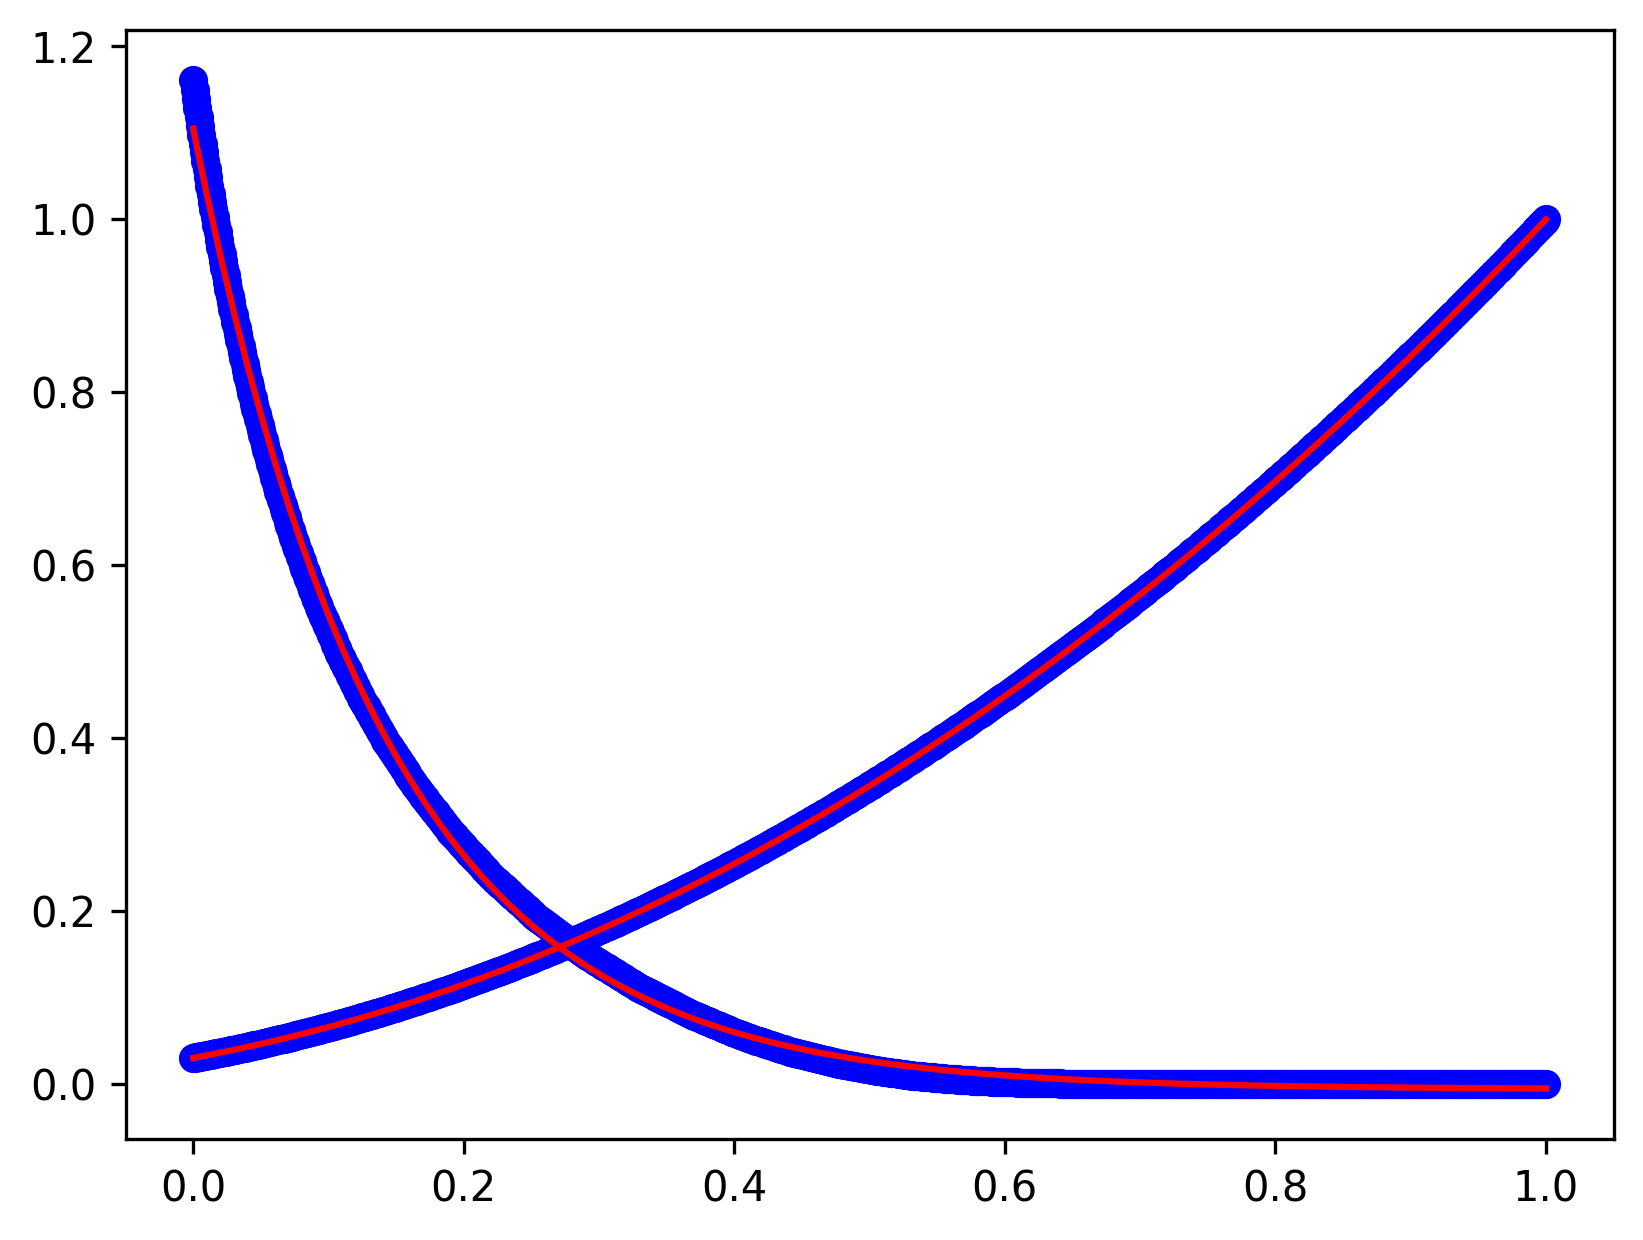
\includegraphics[width=0.8\linewidth]{images/fitted.png}
    \caption{Fitted $A(s)$ and $B(s)$ equations (red) with discrete values (blue) against the normalized annealing fraction $s$}
    \label{fittedequation}
\end{figure}
\chapter{NNQS exploration performance by sizes}\label{appendix:nnqssizegraph}

\section{NAE3SAT}
Refer to \autoref{nnqs-nae3sat-size}.

\begin{figure}[!htb]
    \centering
    \subfloat[Normalized energy]{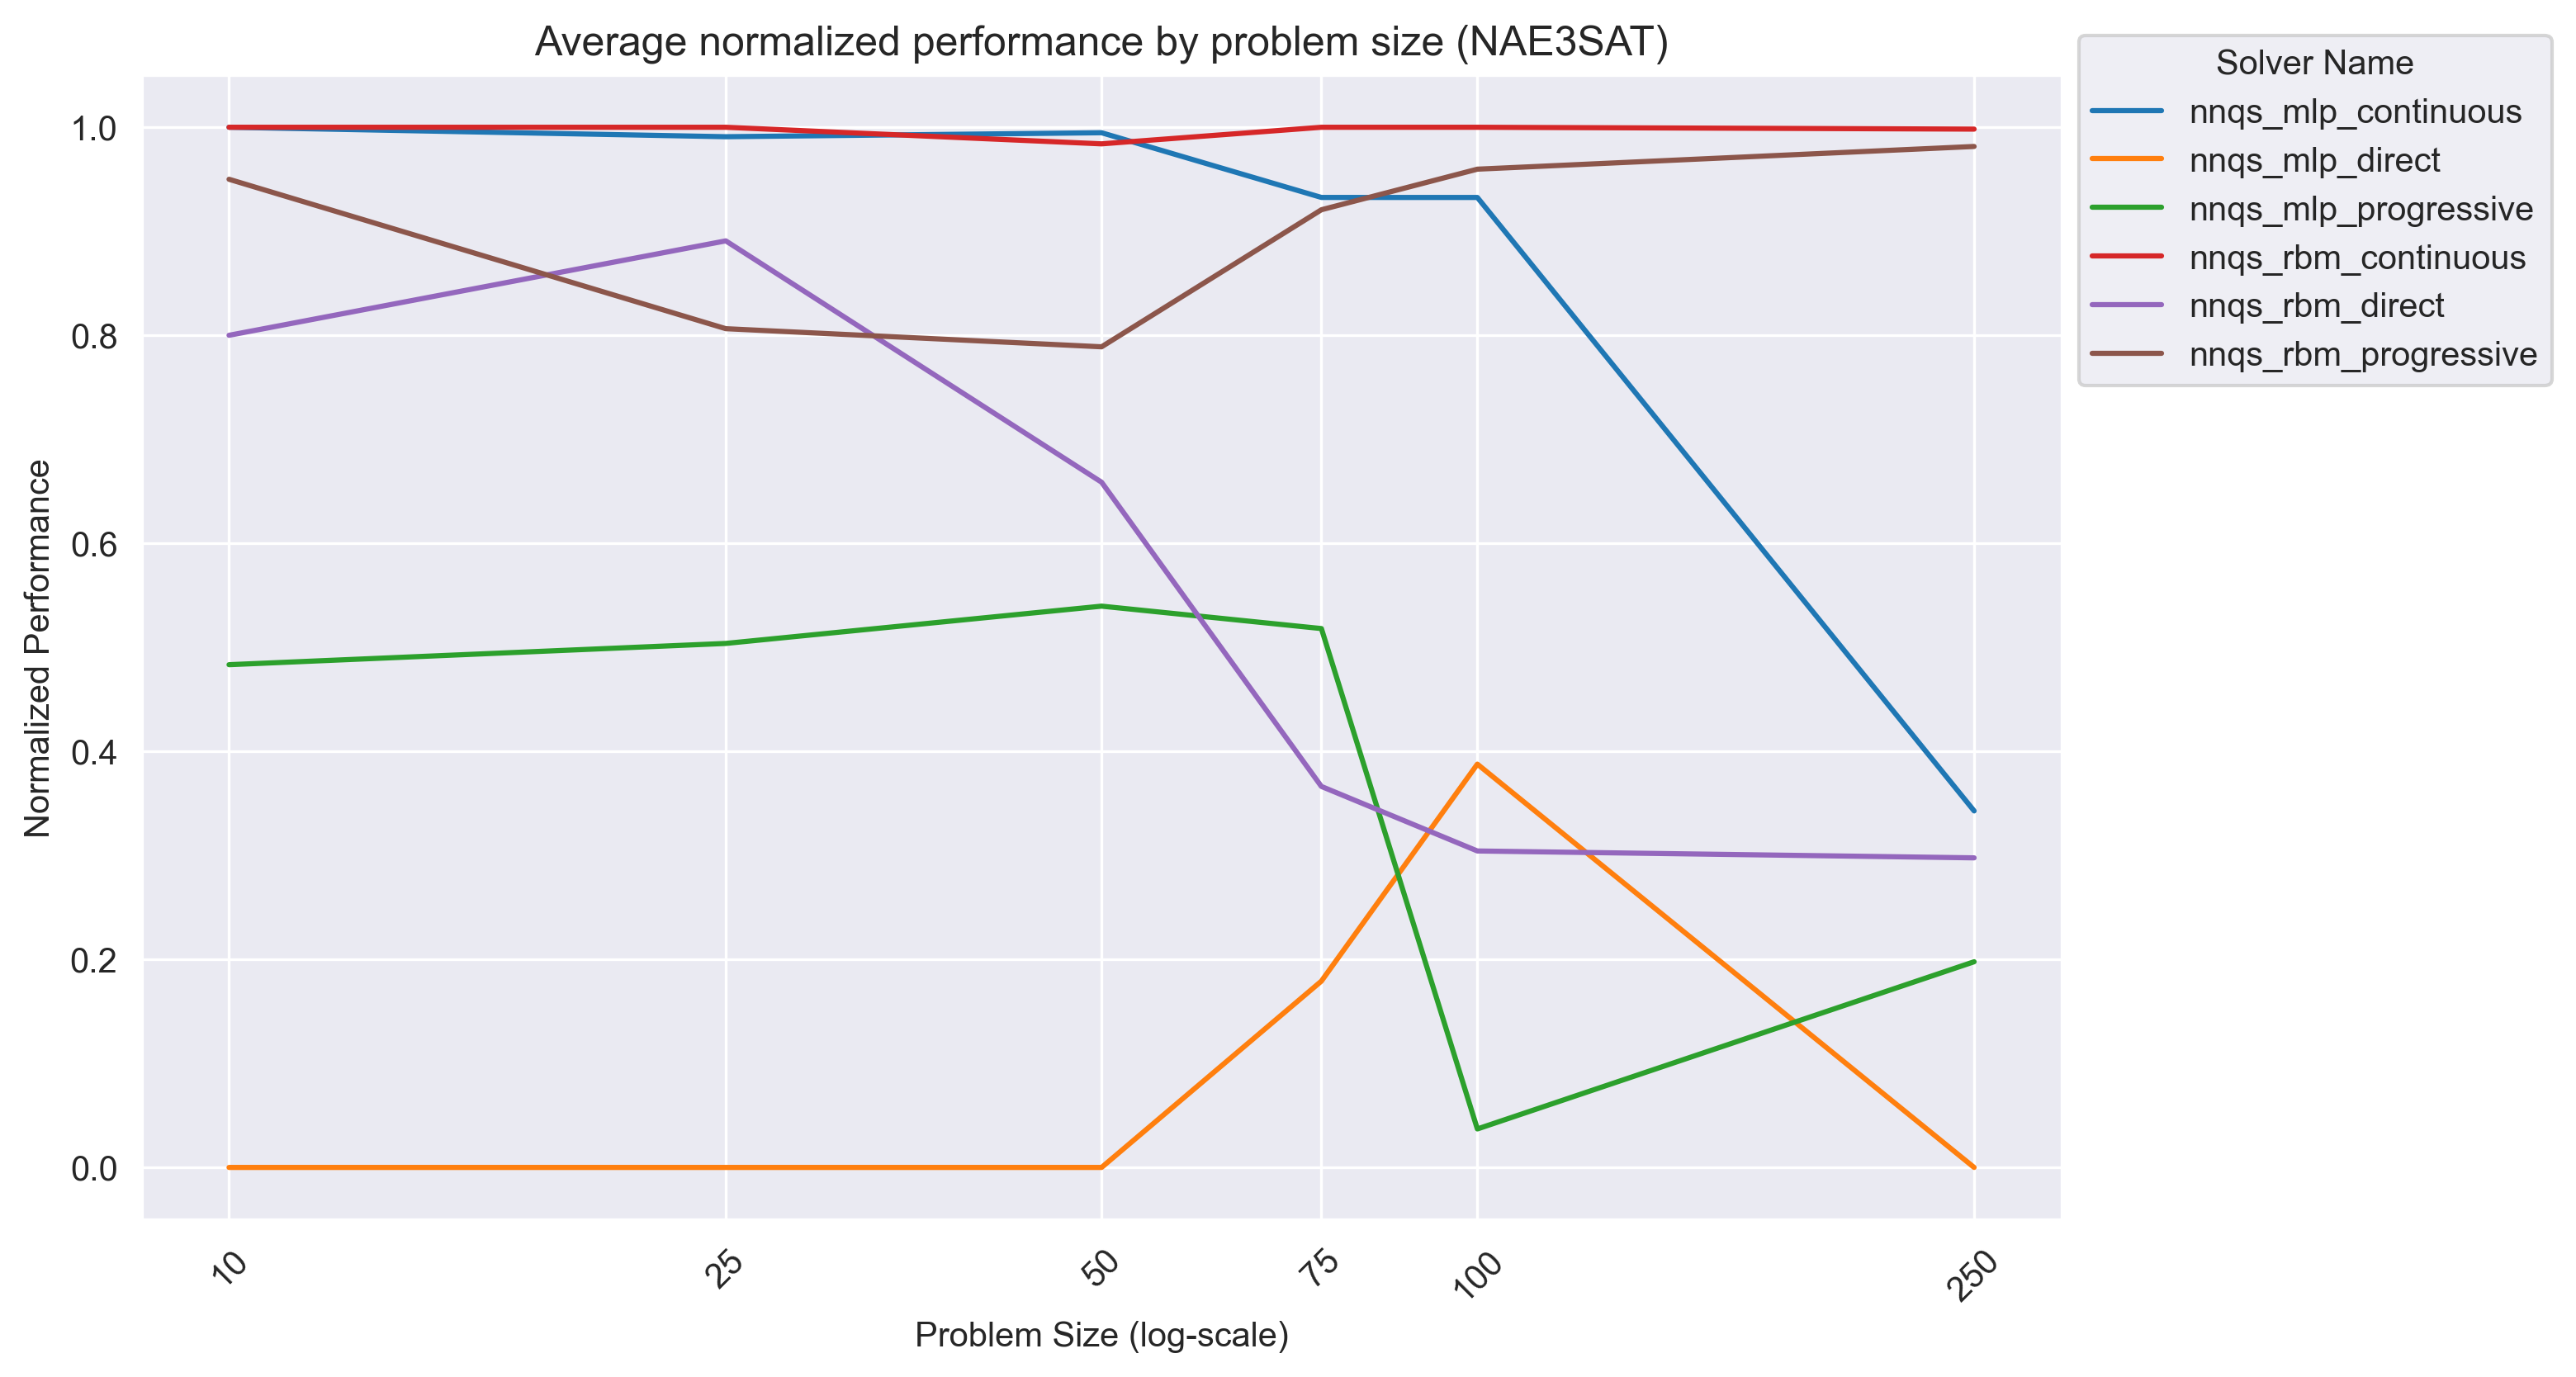
\includegraphics[width=0.8\textwidth]{images/nae3sat_nnqs_size.png}}
    \\
    \subfloat[Success probability]{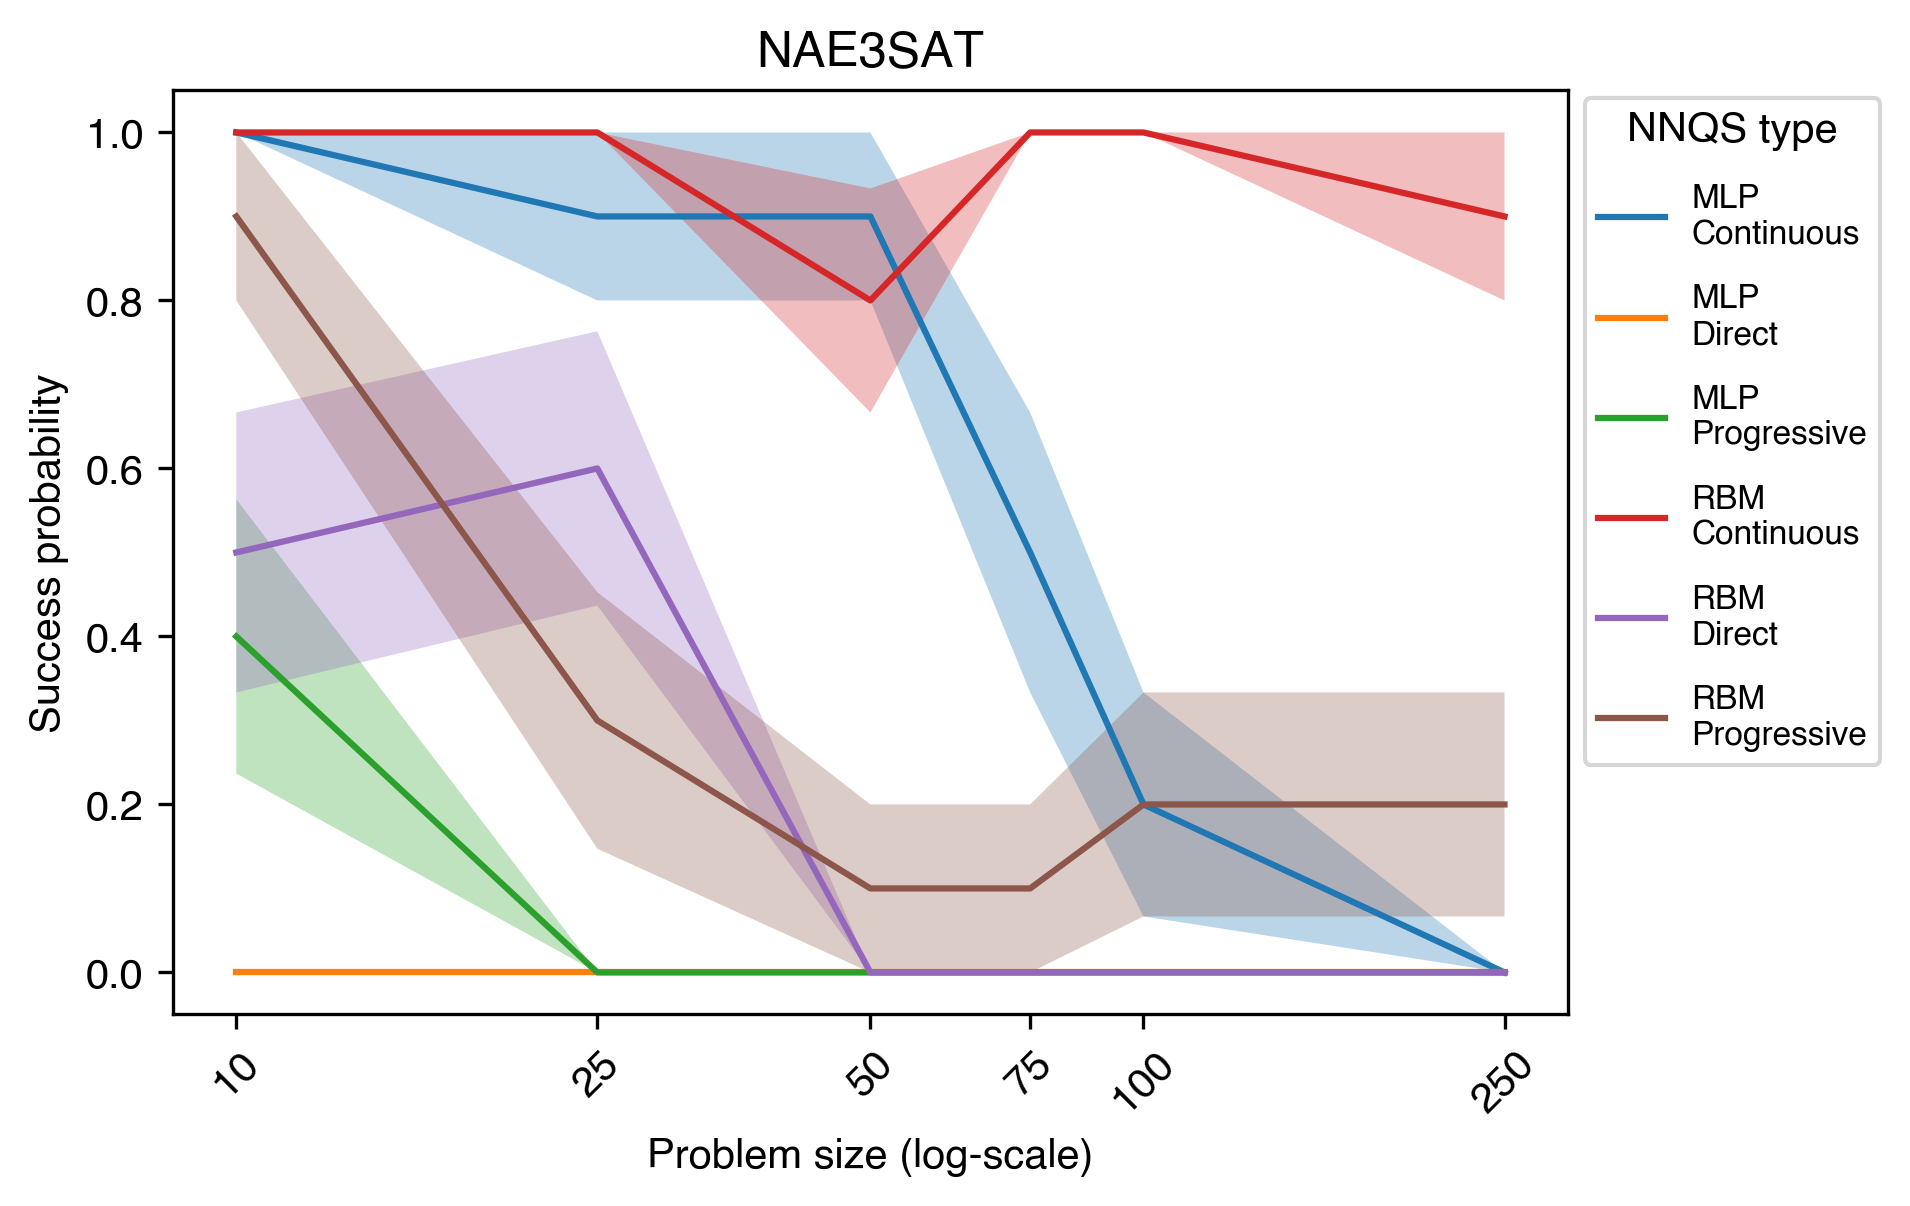
\includegraphics[width=0.8\textwidth]{images/nae3sat_nnqs_success_size.png}}
    \caption{Performance of different NNQS types for NAE3SAT by problem size}
    \label{nnqs-nae3sat-size}
\end{figure}

\section{Max-cut}
Refer to \autoref{nnqs-maxcut-size}.

\begin{figure}[!htb]
    \centering
    \subfloat[Normalized energy]{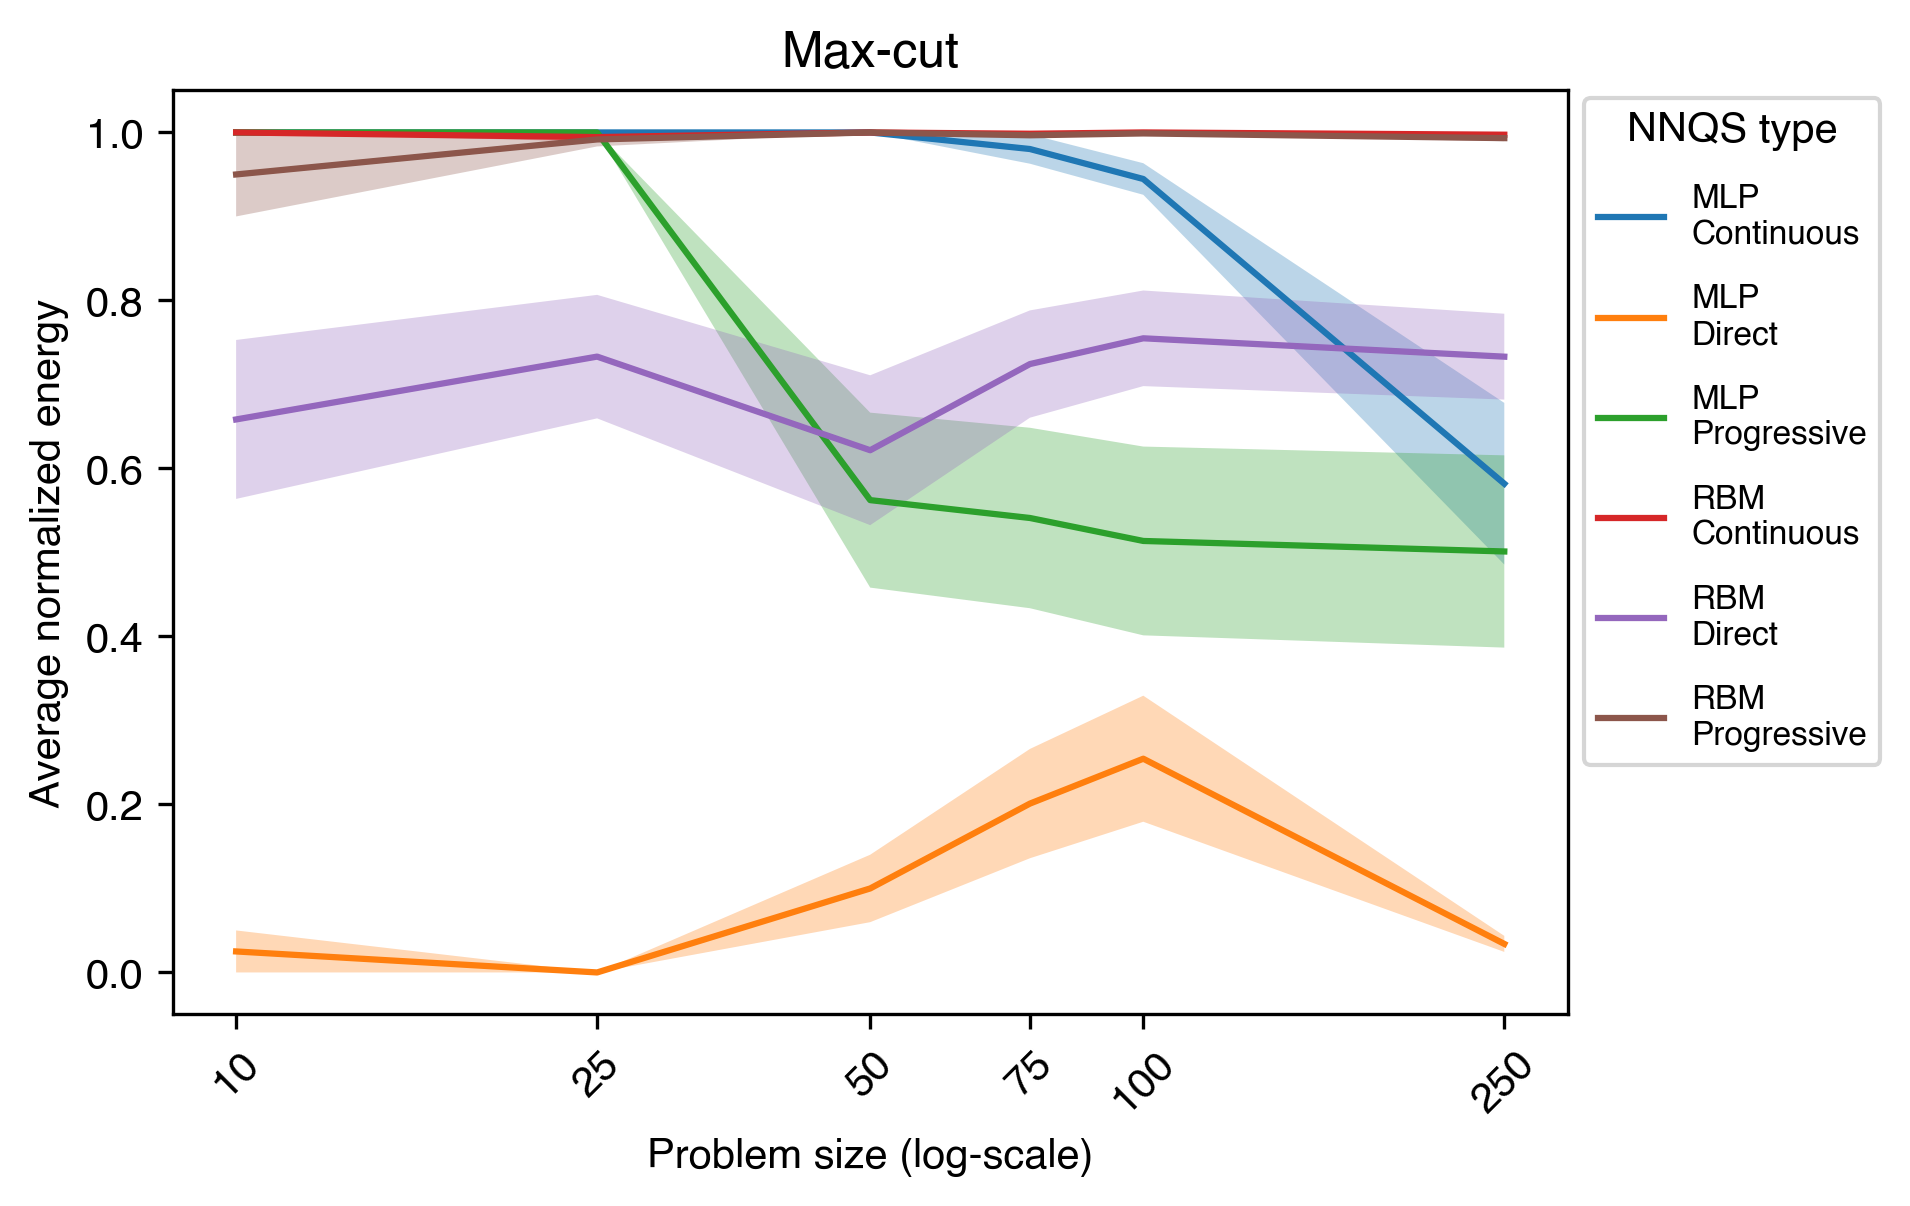
\includegraphics[width=0.8\textwidth]{images/maxcut_nnqs_size.png}}
    \\
    \subfloat[Success probability]{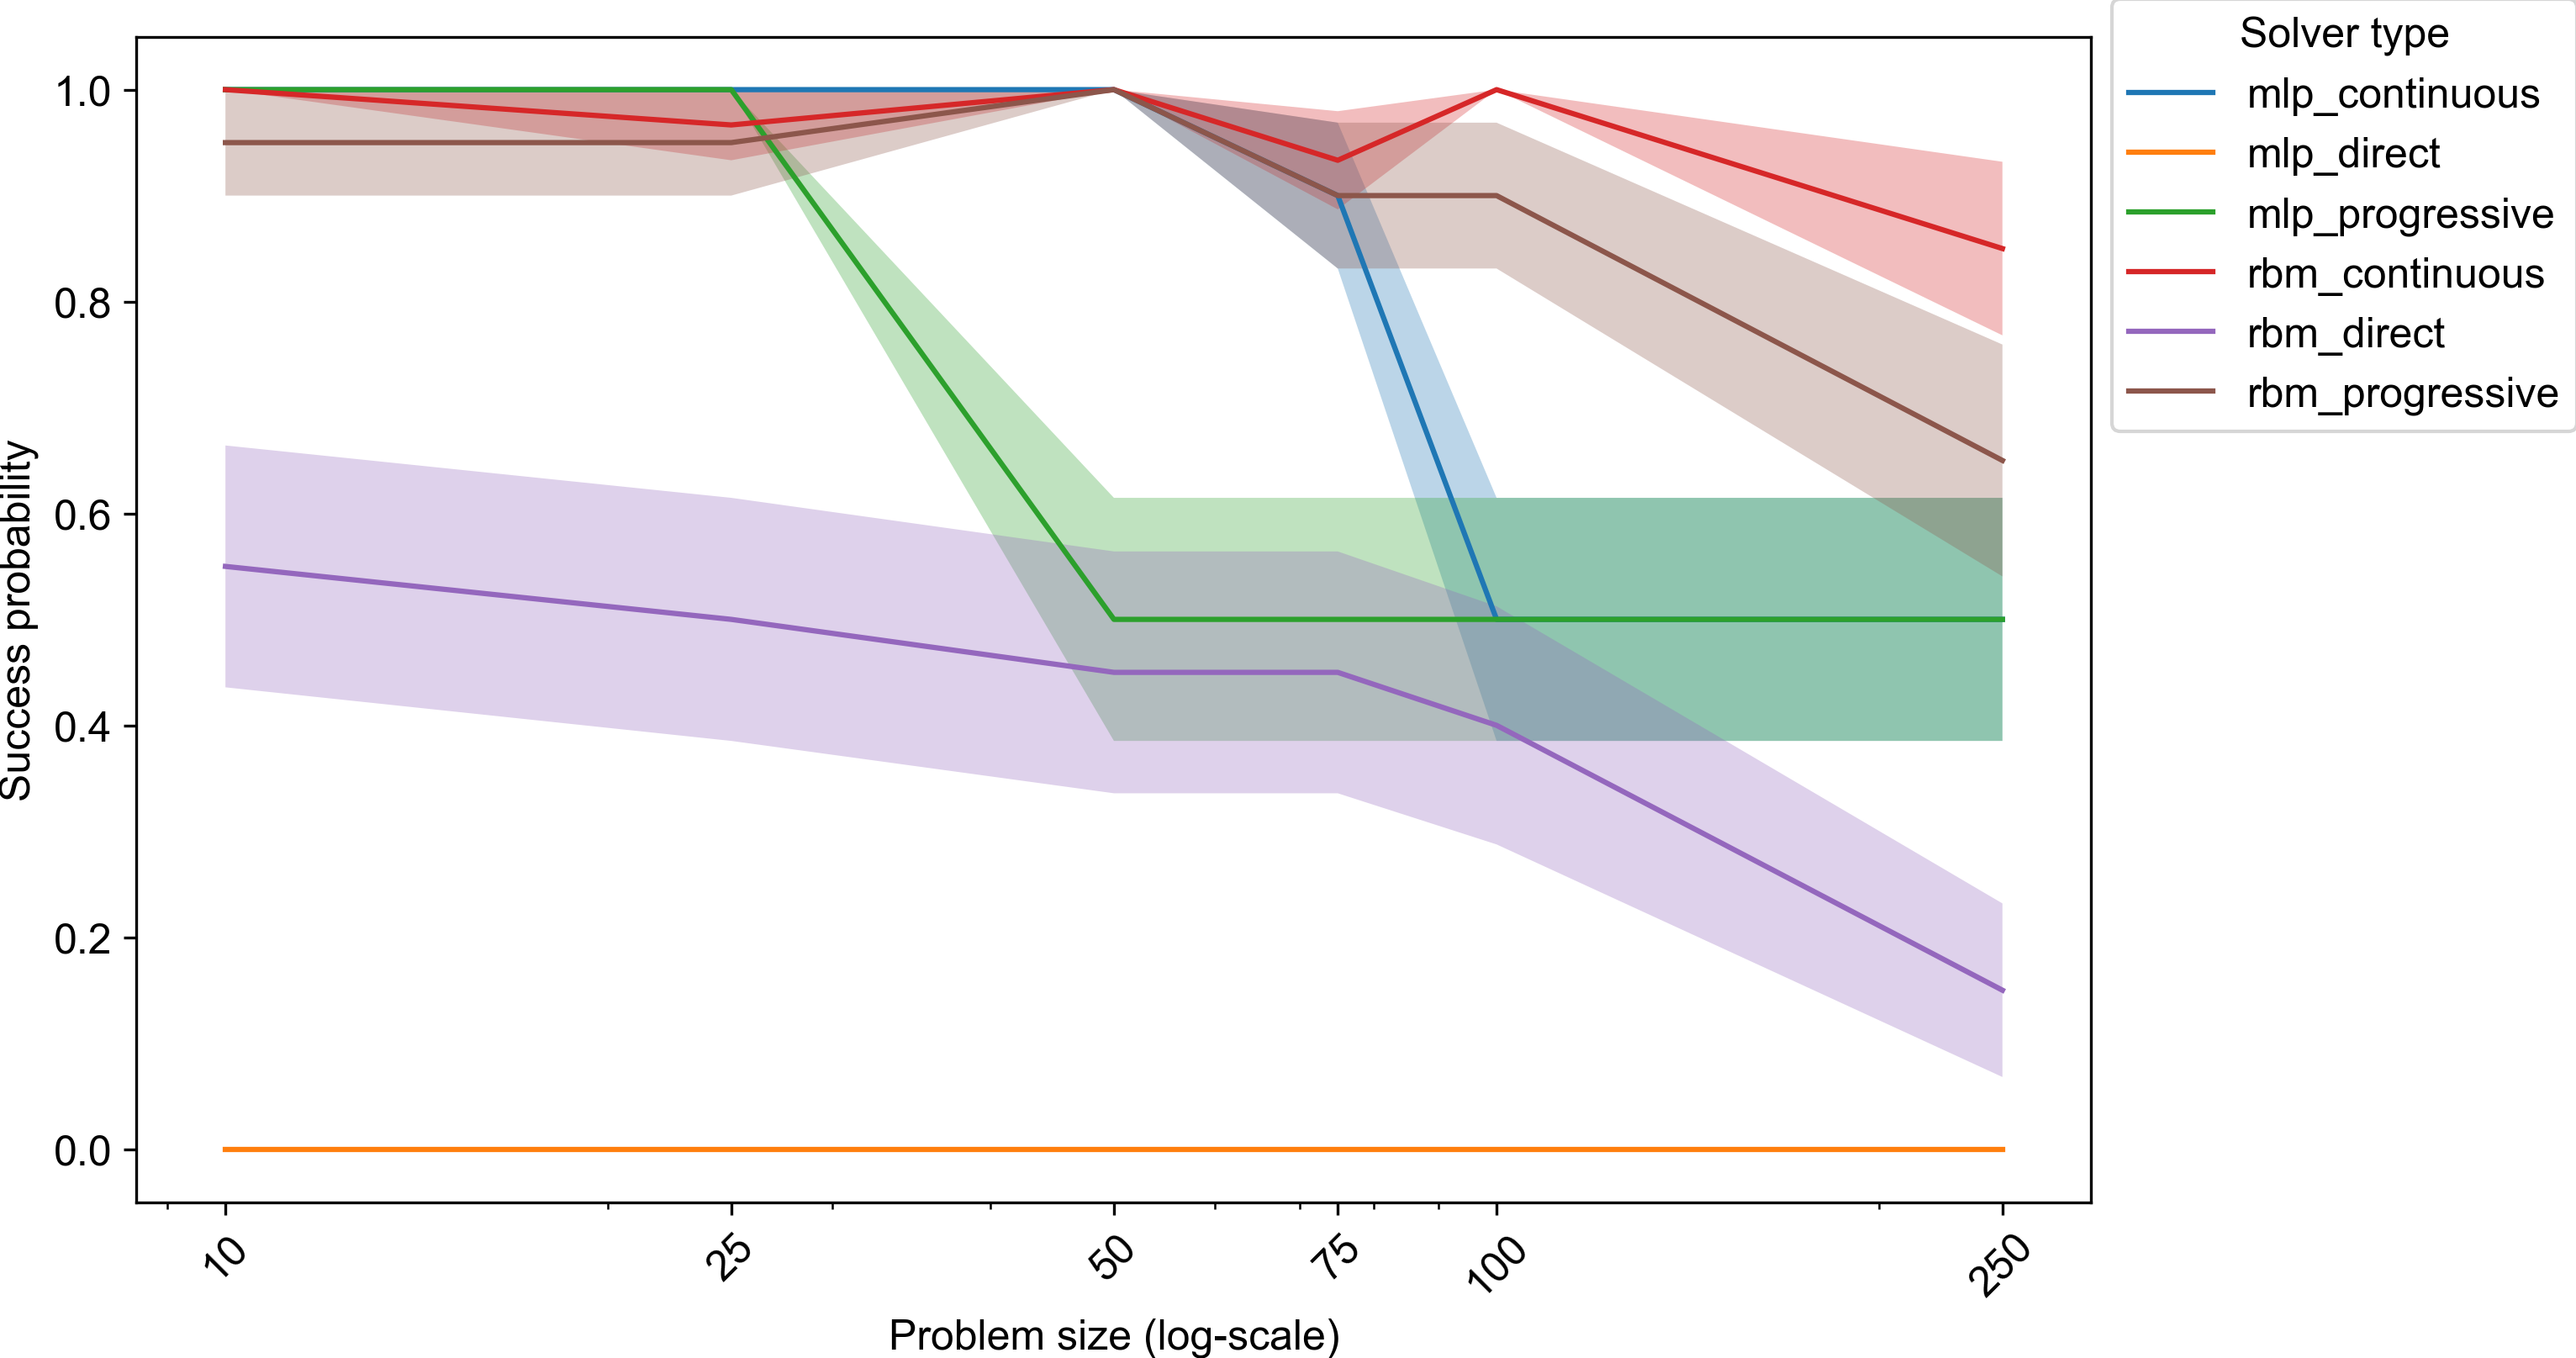
\includegraphics[width=0.8\textwidth]{images/maxcut_nnqs_success_size.png}}
    \caption{Performance of different NNQS types for max-cut by problem size}
    \label{nnqs-maxcut-size}
\end{figure}

\section{SK model}
Refer to \autoref{nnqs-skmodel-size}.

\begin{figure}[!htb]
    \centering
    \subfloat[Normalized energy]{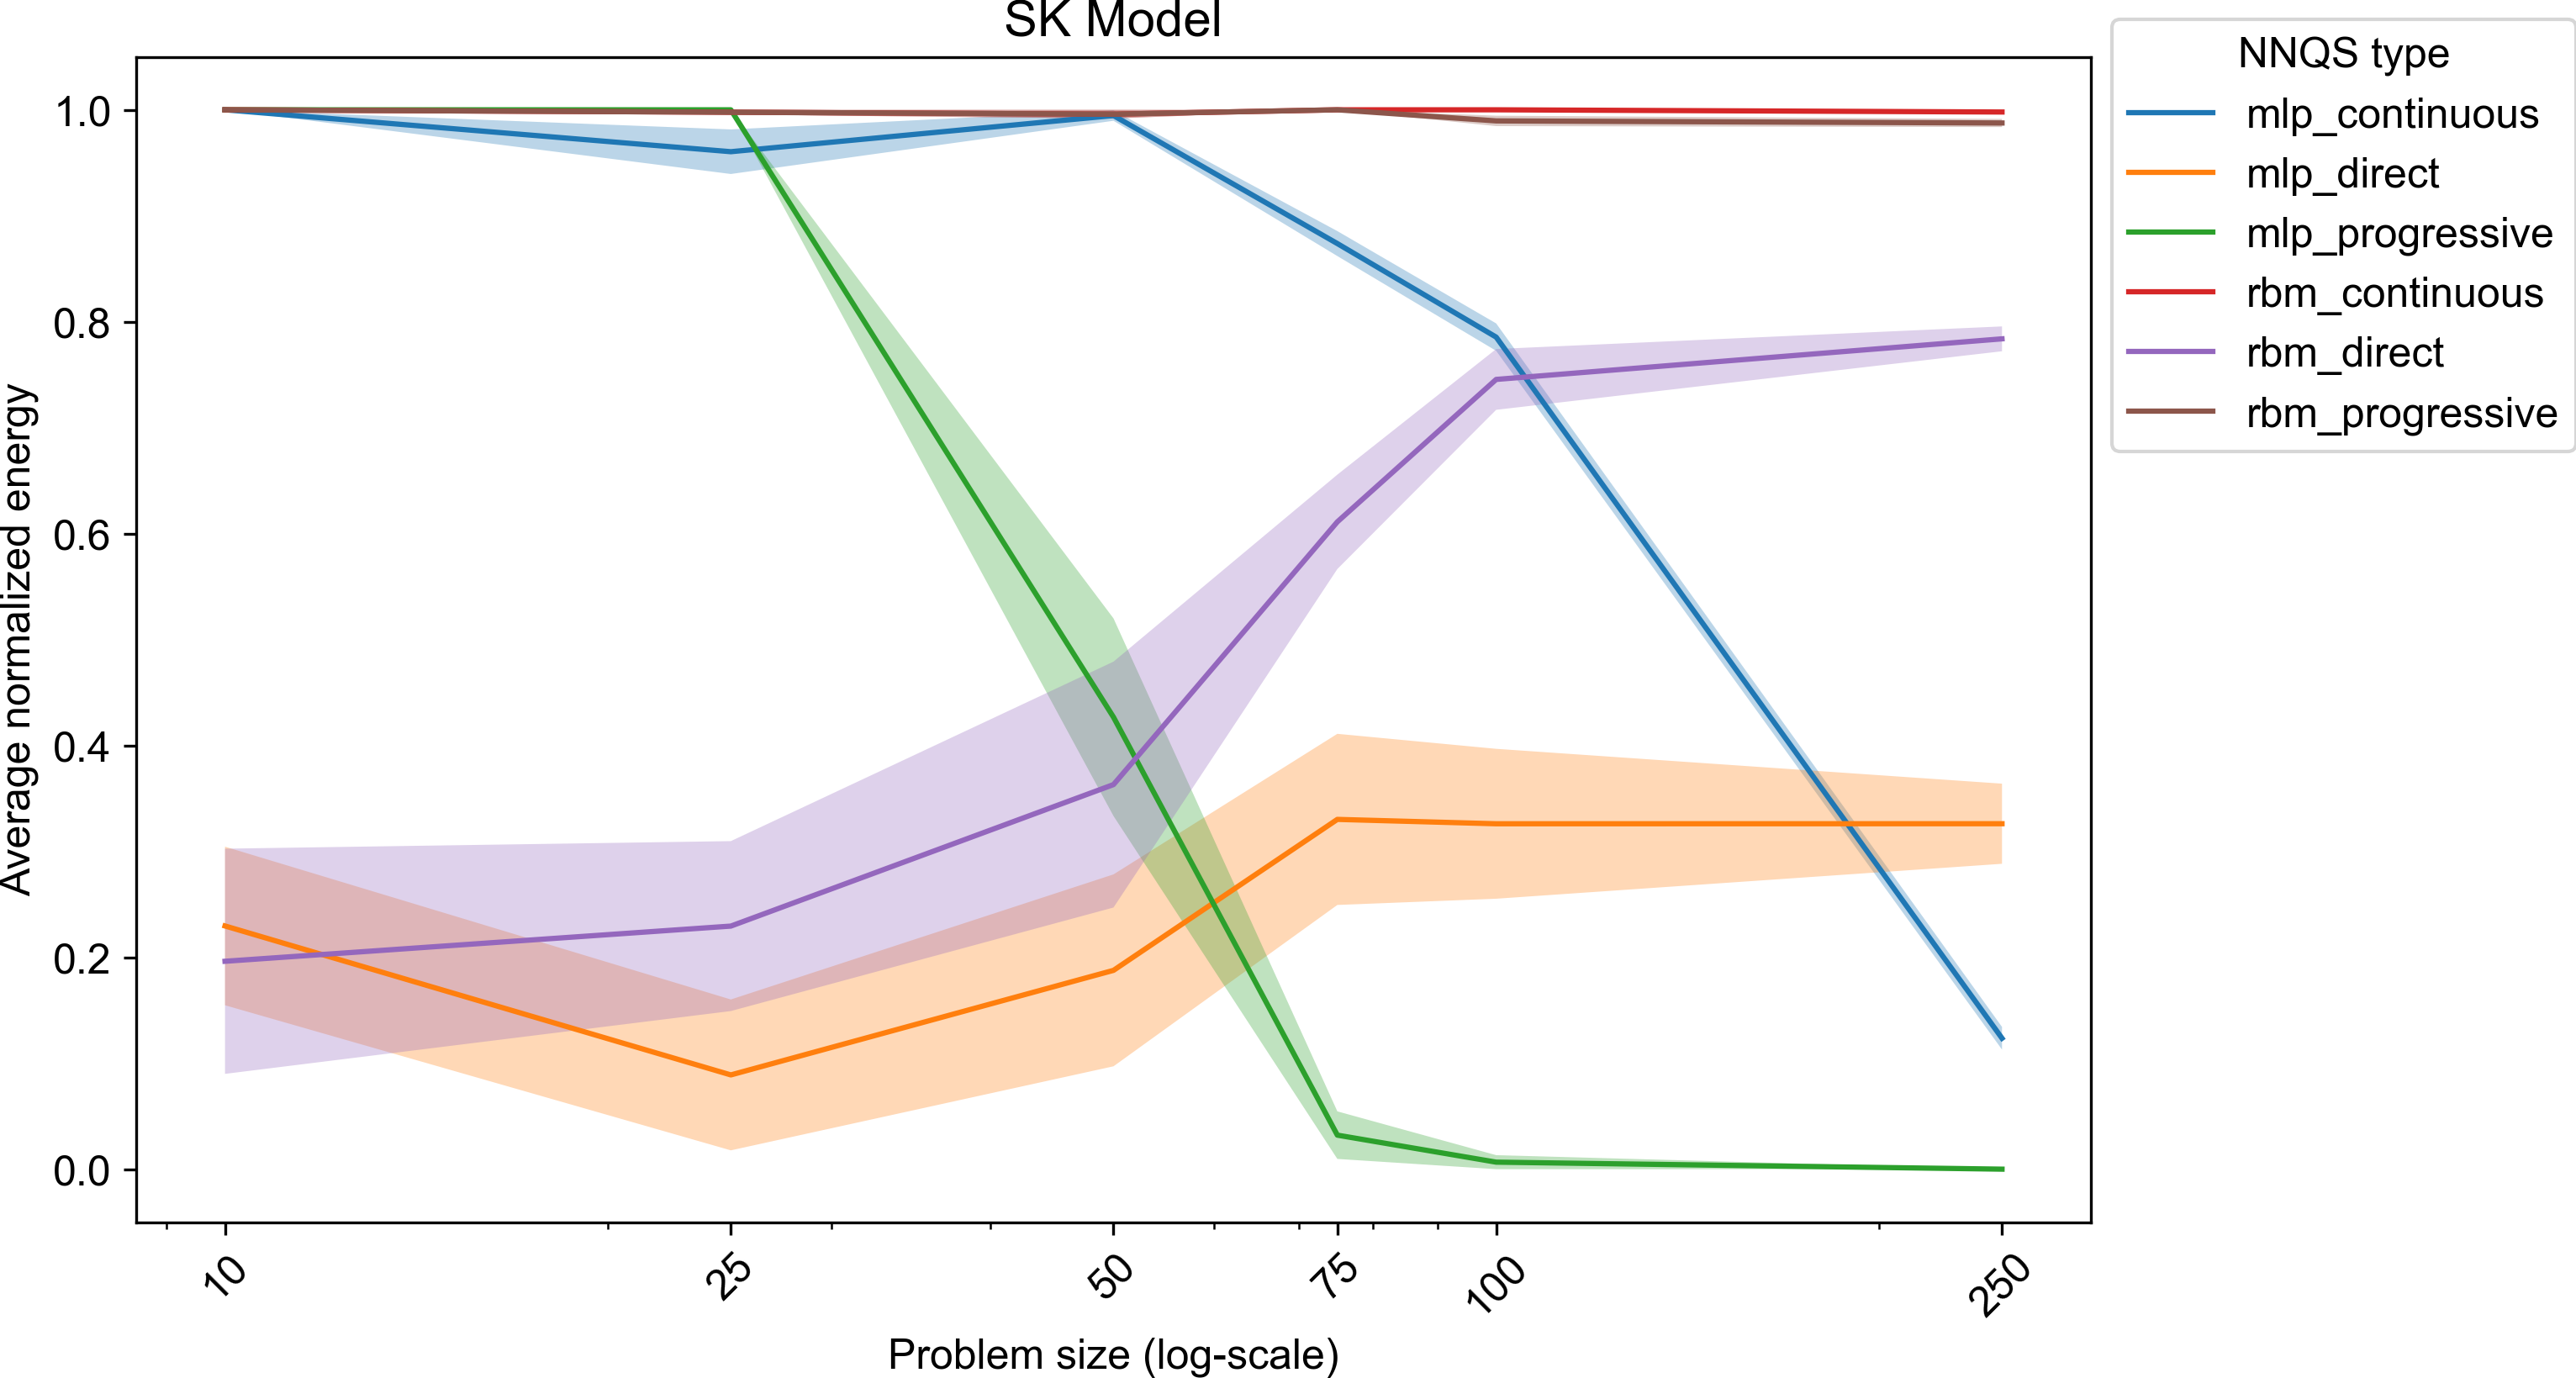
\includegraphics[width=0.8\textwidth]{images/skmodel_nnqs_size.png}}%\hfill
    \\
    \subfloat[Success probability]{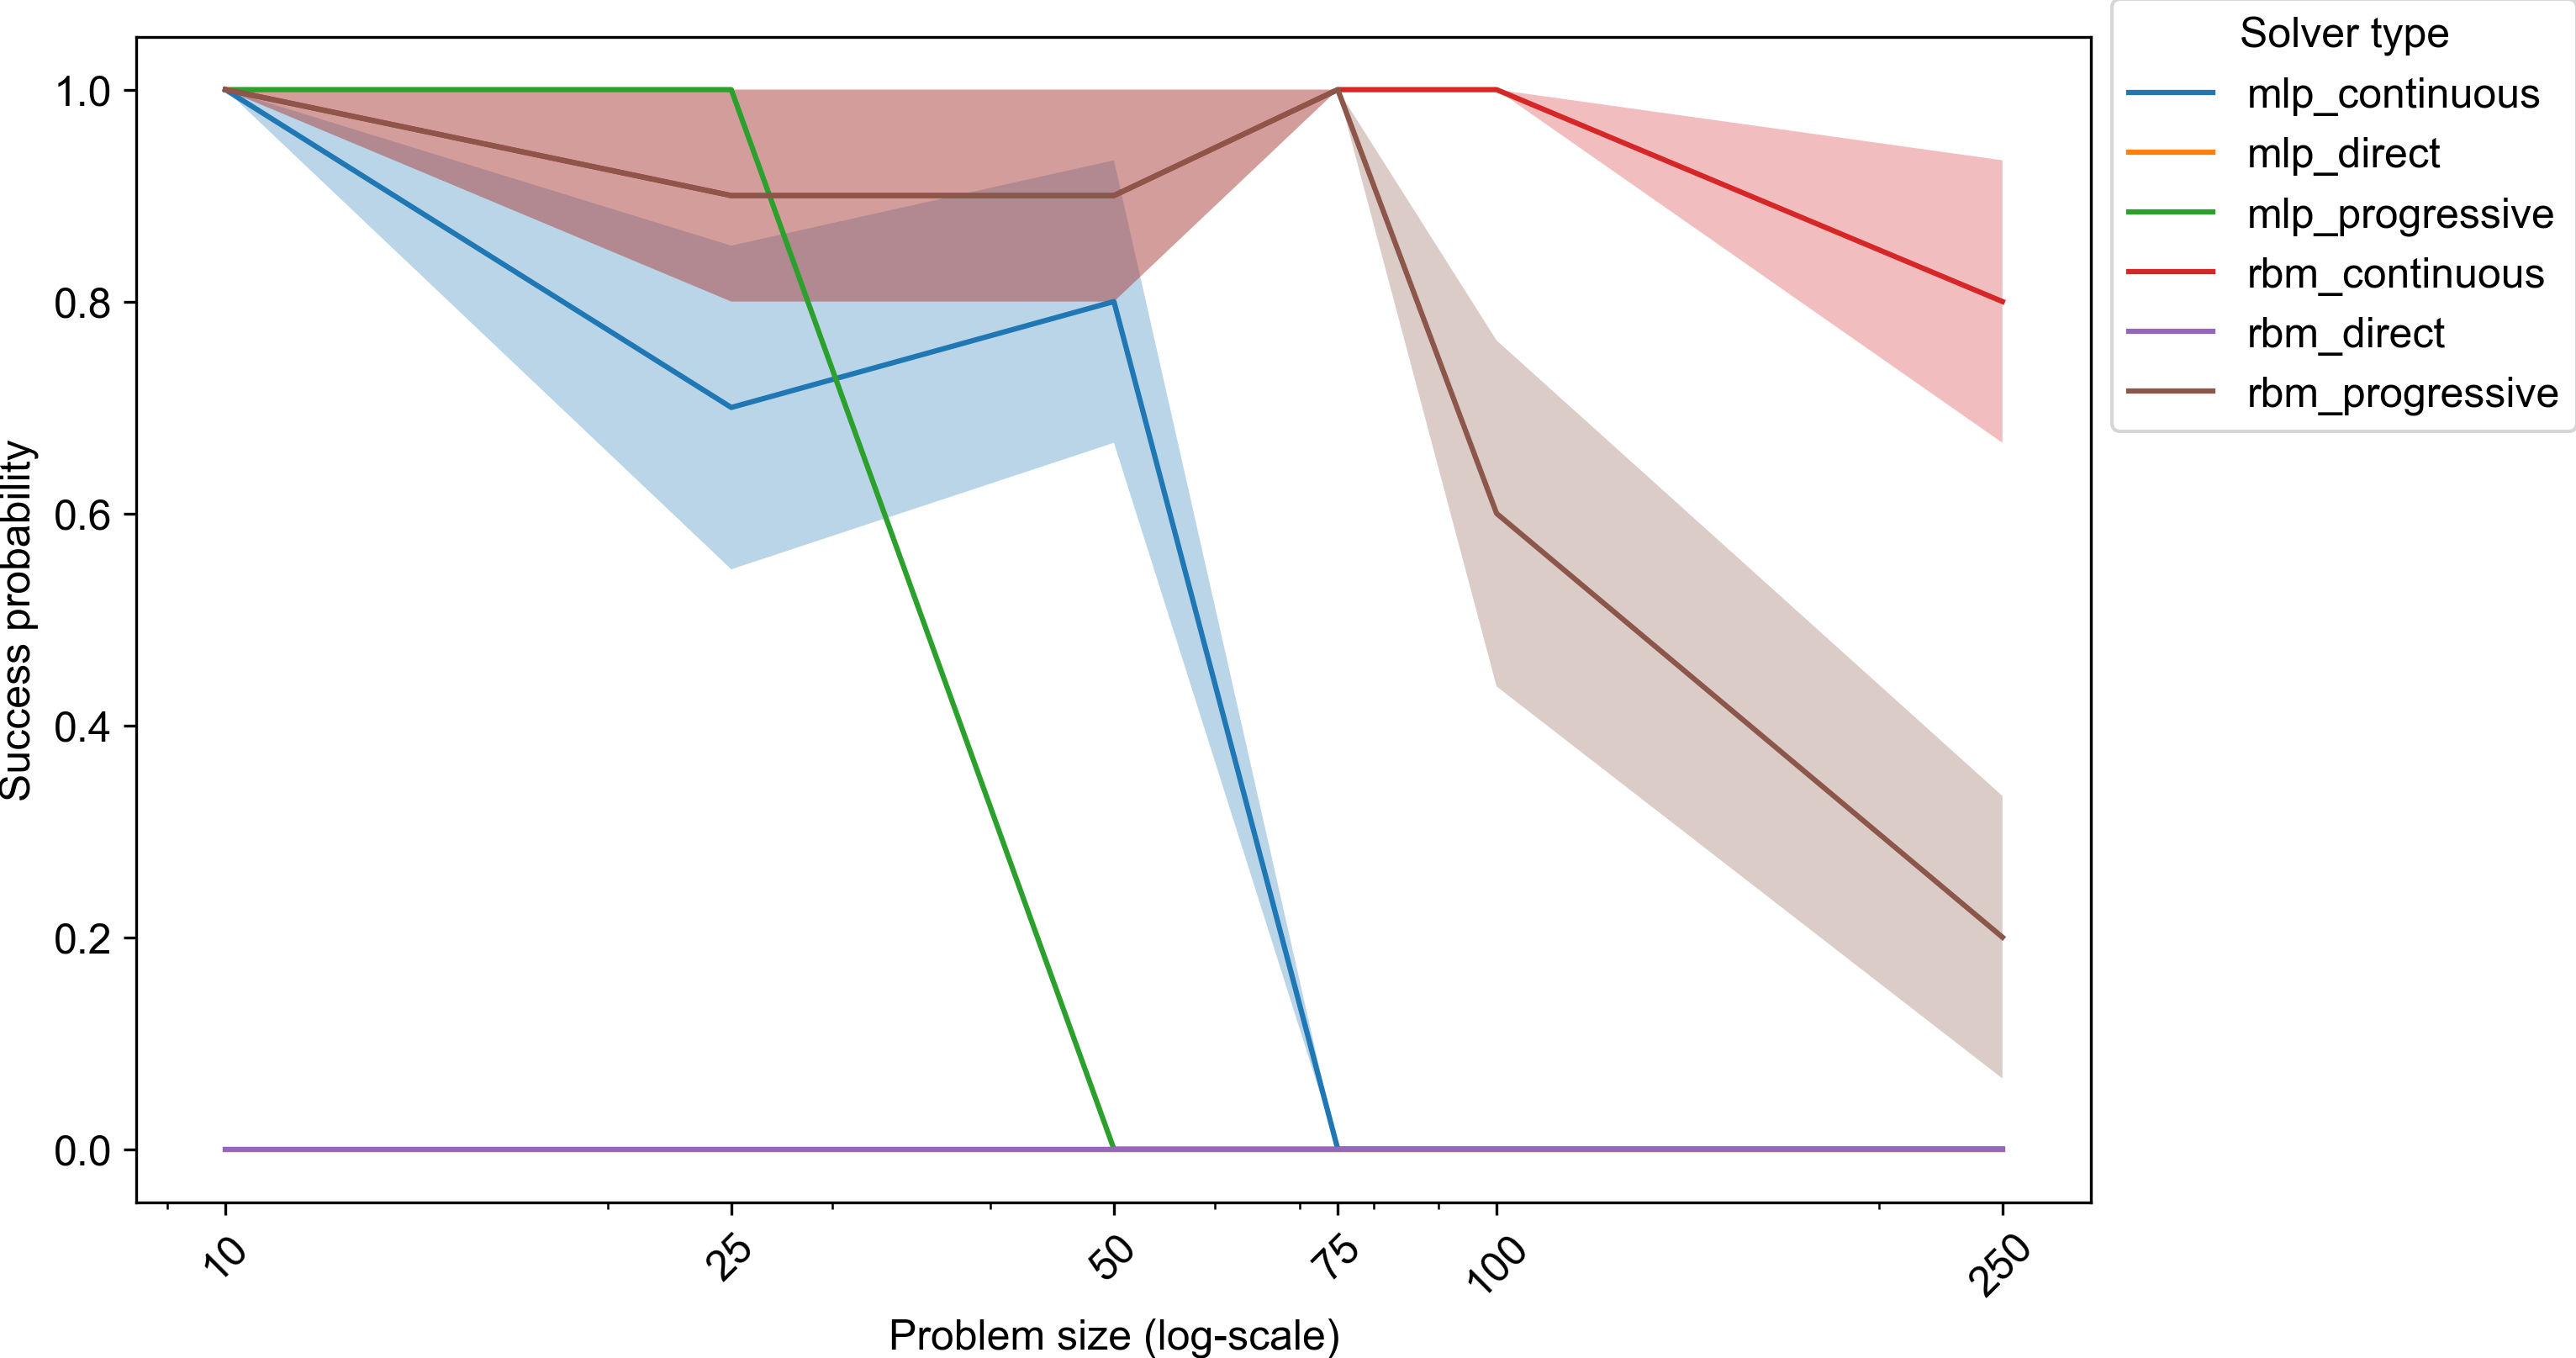
\includegraphics[width=0.8\textwidth]{images/skmodel_nnqs_success_size.png}}
    \caption{Performance of different NNQS types for SK model by problem size}
    \label{nnqs-skmodel-size}
\end{figure}
\chapter{Average runtime of solvers by problem type and sizes}\label{appendix:timesizegraph}

\section{NAE3SAT}
\autoref{time-nae3sat-size} shows the average runtime taken for NAE3SAT problems.
\begin{figure}[!h]
    \centering
    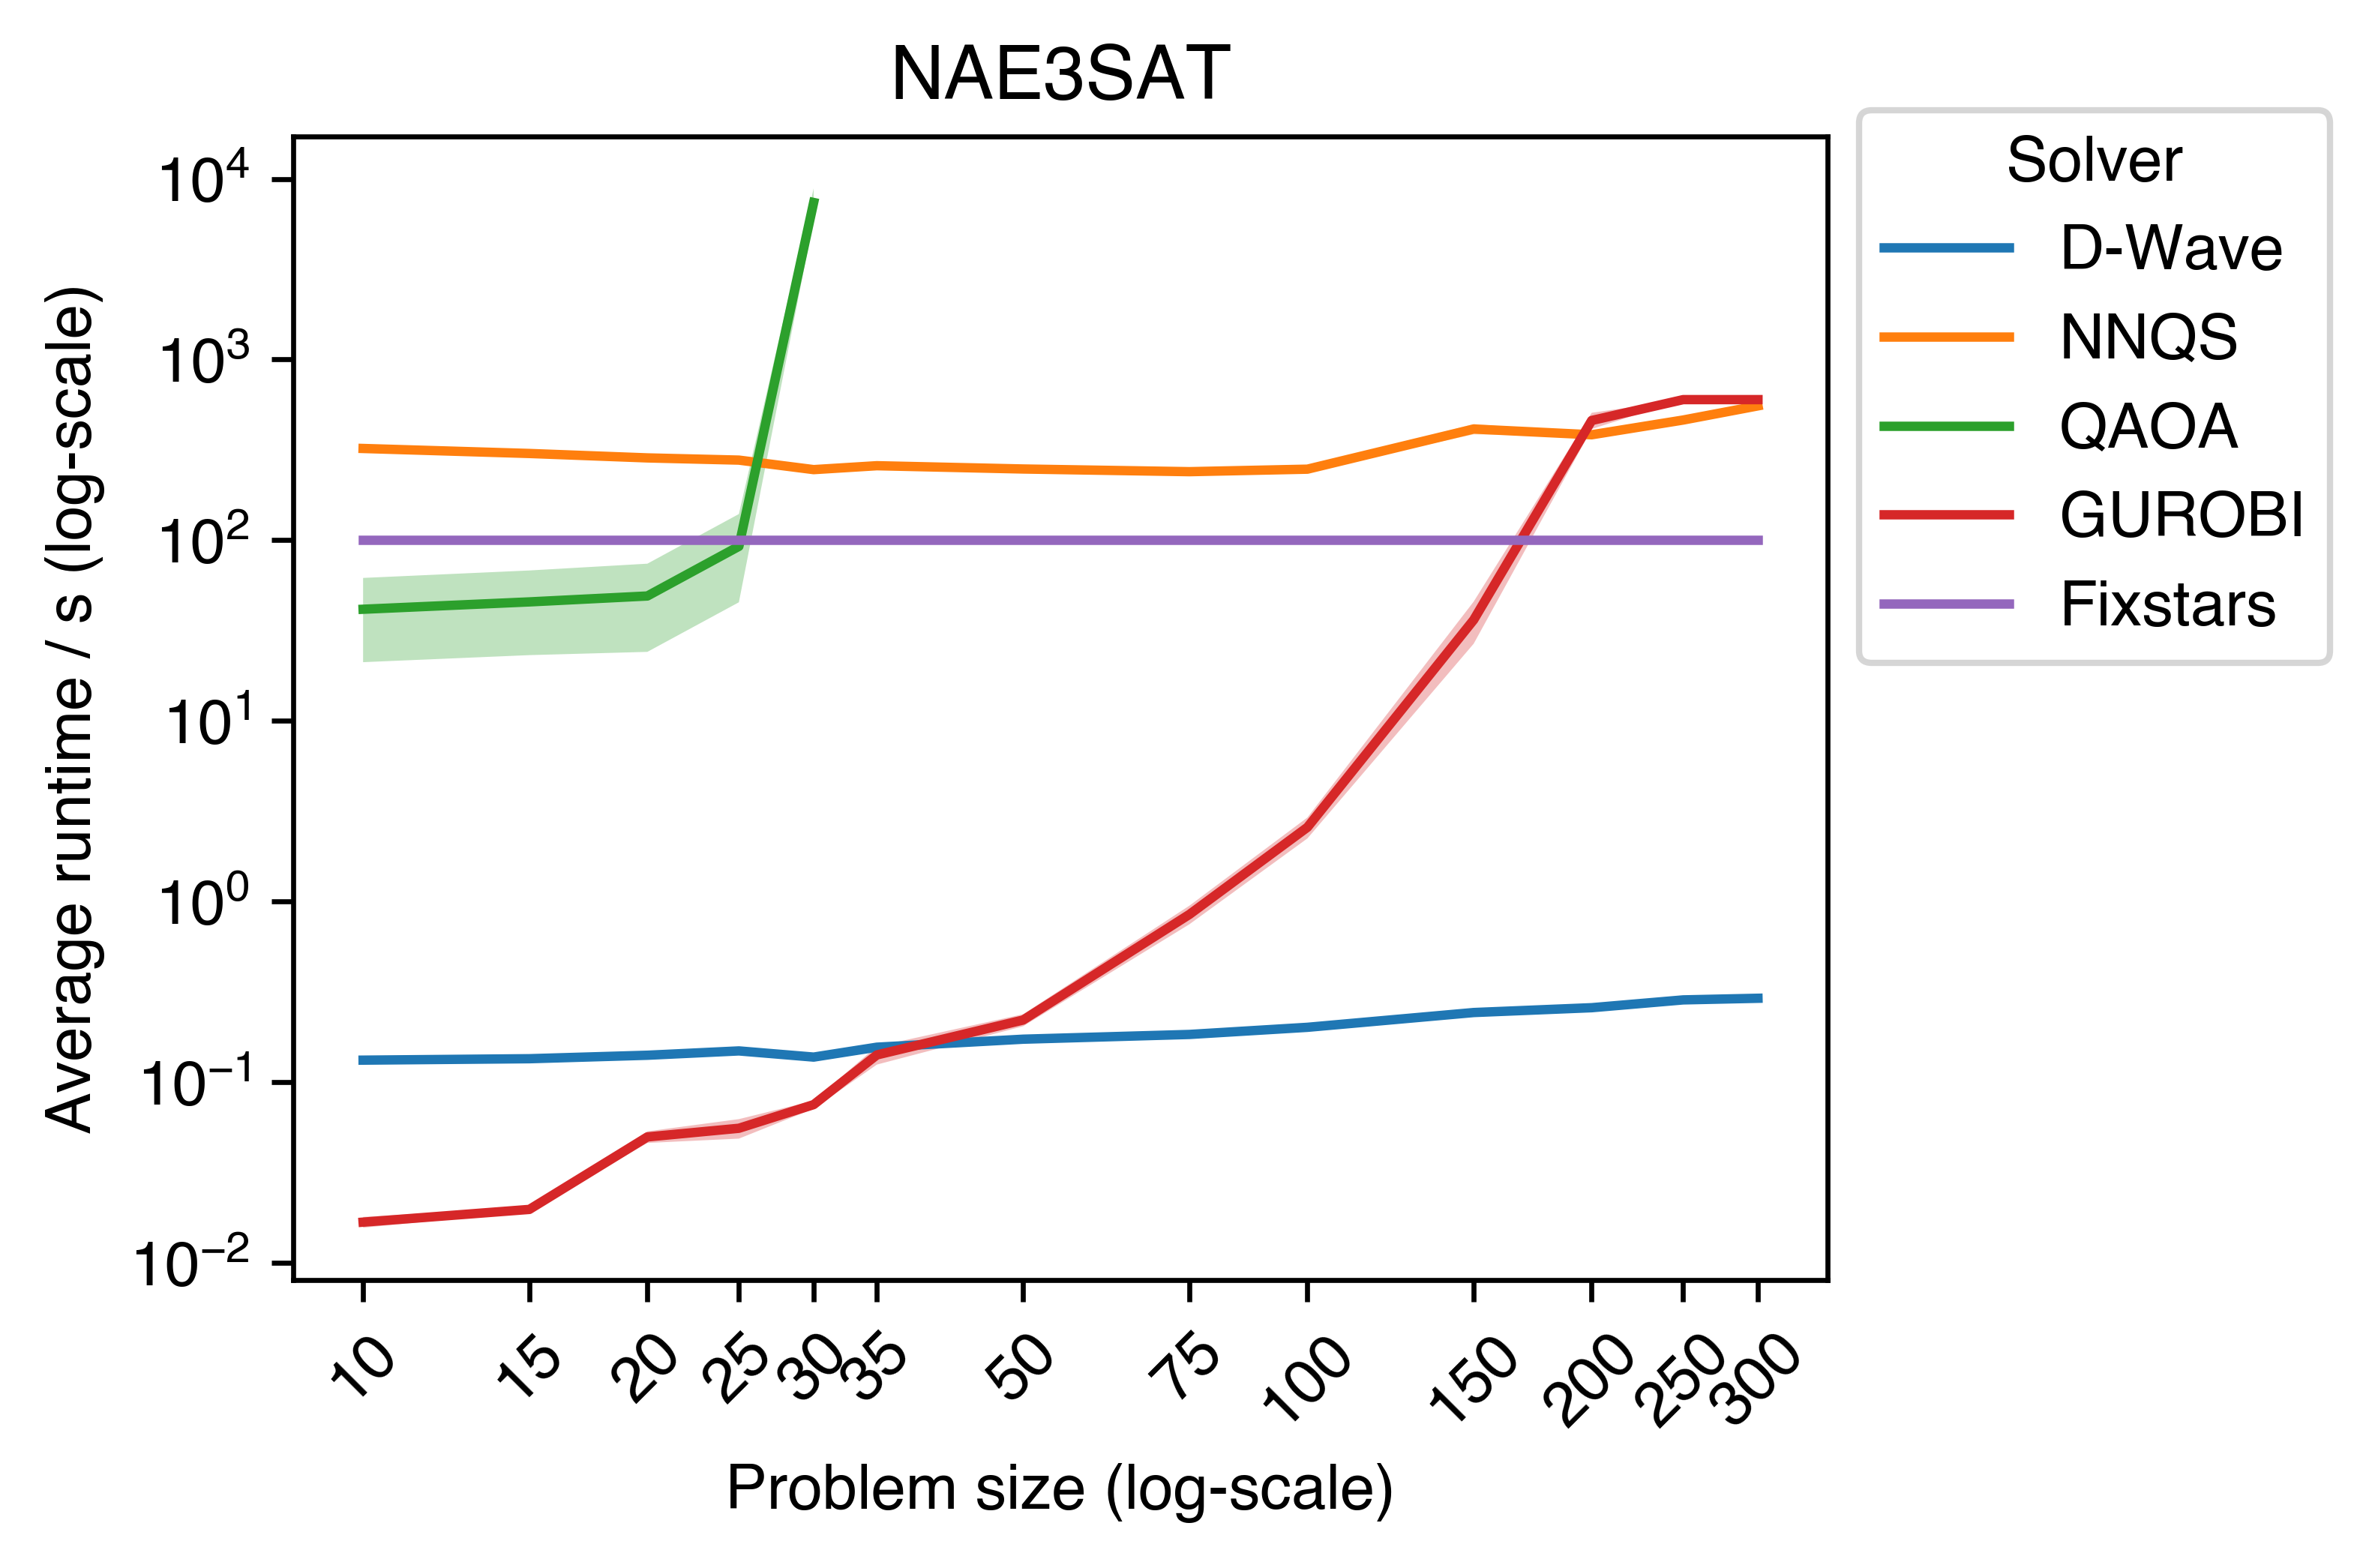
\includegraphics[width=0.8\textwidth]{images/nae3sat_all_time_size.png}
    \caption{Average runtime taken by different solvers for NAE3SAT by problem size}
    \label{time-nae3sat-size}
\end{figure}

\section{Max-cut}
\autoref{time-maxcut-size} shows the average runtime taken for max-cut problems.
\begin{figure}[!h]
    \centering
    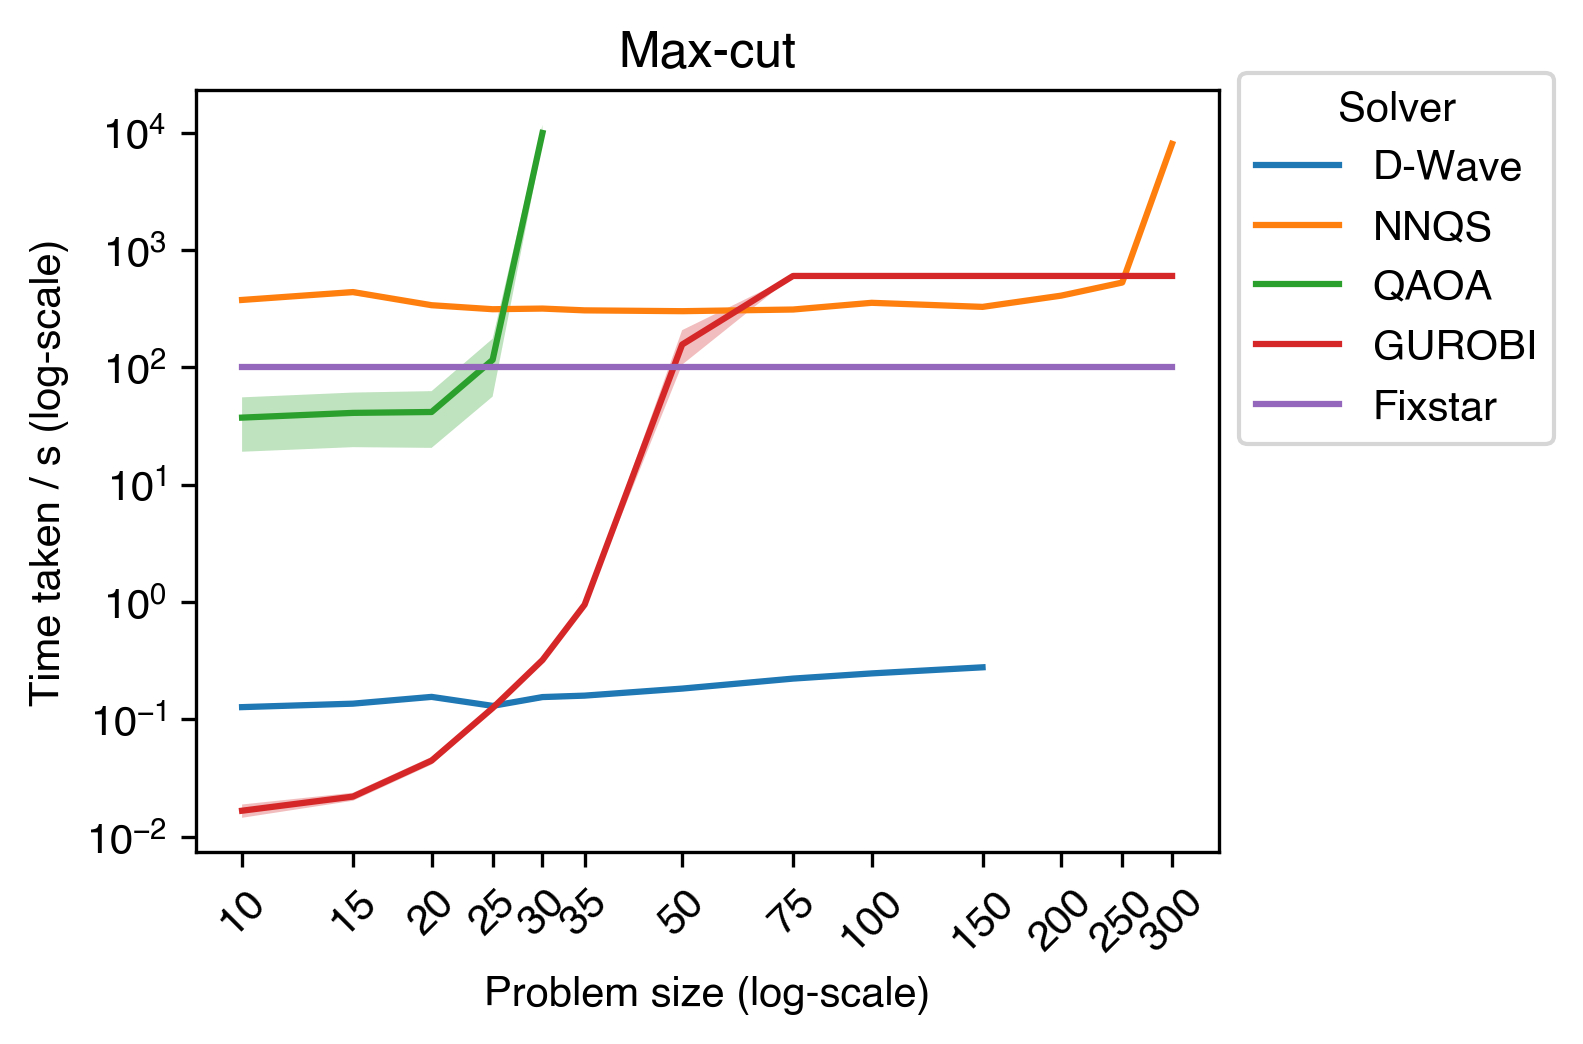
\includegraphics[width=0.8\textwidth]{images/maxcut_all_time_size.png}
    \caption{Average runtime taken by different solvers for max-cut by problem size}\label{time-maxcut-size}
\end{figure}

\section{SK model}
\autoref{time-skmodel-size} shows the average runtime taken for SK model problems.
\begin{figure}[!h]
    \centering
    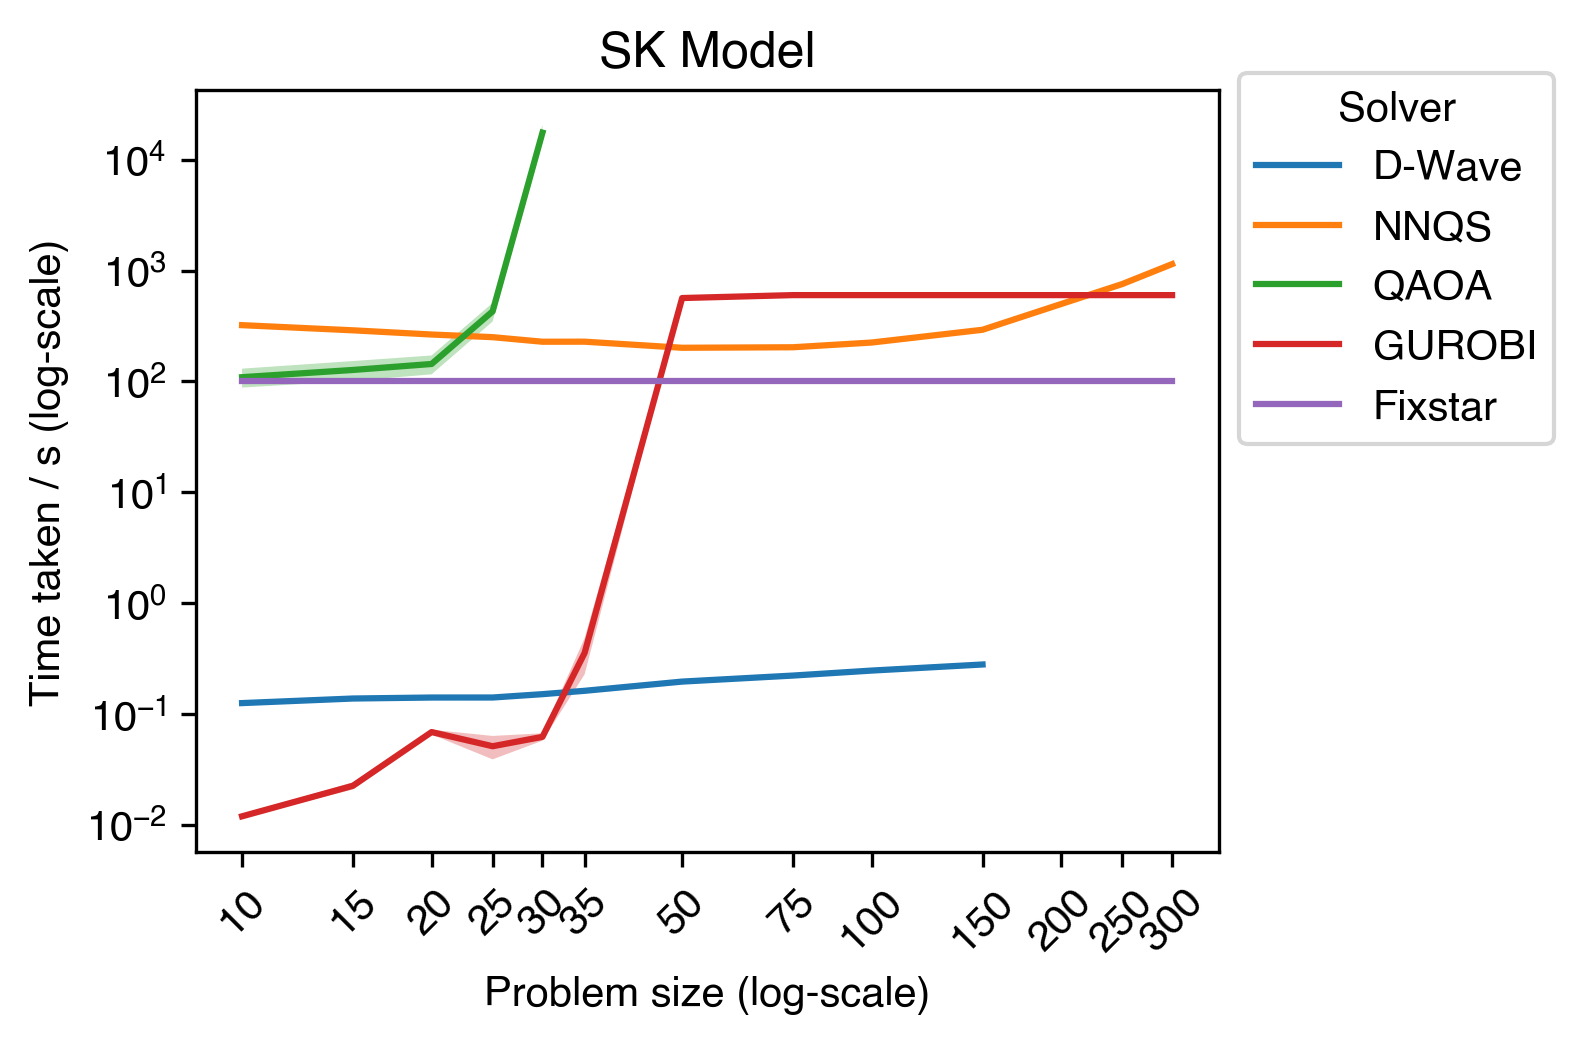
\includegraphics[width=0.8\textwidth]{images/skmodel_all_time_size.png}
    \caption{Average runtime taken by different solvers for SK model by problem size}    \label{time-skmodel-size}
\end{figure}
\chapter{Metadata of solvers by problem type and sizes}\label{appendix:metadata}

\section{D-wave}
For the D-wave solver, we recorded the average number of embedded qubits which is needed during the minor embedding phase shown in \autoref{table:numberofembedded}.

\begin{table}[!ht]
    \centering
    \resizebox{\textwidth}{!}{%
    \begin{tabular}{lrrrrrrrrrrrrr} \toprule
        $n$ & 10 & 15 & 20 & 25 & 30 & 35 & 50 & 75 & 100 & 150 & 200 & 250 & 300 \\ \midrule
        NAE3SAT & 15.15 & 27.90 & 42.20 & 58.85 & 80.90 & 102.25 & 184.05 & 379.65 & 622.15 & 1381.00 & 2322.65 & 3756.20 & 4493.60 \\
        Max-cut & 12.70 & 25.95 & 45.45 & 69.90 & 102.60 & 142.50 & 304.05 & 706.05 & 1290.00 & 3087.95 & - & - & - \\
        SK model & 17.05 & 35.80 & 54.50 & 87.65 & 121.15 & 169.80 & 331.60 & 739.45 & 1338.65 & 2995.25 & - & - & - \\ \bottomrule
    \end{tabular}}
    \caption{Average number of embedded qubits for the D-wave solver by problem type and size}
    \label{table:numberofembedded}
\end{table}

\section{QAOA}
For the D-wave solver, we recorded the average number of quantum gates and the circuit depth shown in \autoref{table:gates} and \autoref{table:depth} which help to quantify the complexity of the quantum circuit.

\begin{table}[!ht]
    \centering
    \begin{tabular}{lrrrrr} \toprule
        $n$ & 10 & 15 & 20 & 25 & 30\\ \midrule
        NAE3SAT & 77.75 & 127.80 & 181.50 & 235.20 & 292.30 \\
        Max-cut & 75.00 & 131.00 & 200.00 & 281.00 & 375.00 \\
        SK model & 95.00 & 180.00 & 290.00 & 425.00 & 585.00\\ \bottomrule
    \end{tabular}
    \caption{Average number of quantum gates in the quantum circuit used by the QAOA solver by problem type and size}
    \label{table:gates}
\end{table}

\begin{table}[!ht]
    \centering
    \begin{tabular}{lrrrrr} \toprule
        $n$ & 10 & 15 & 20 & 25 & 30\\ \midrule
        NAE3SAT & 18.65 & 25.30 & 30.70 & 35.15 & 40.00 \\
        Max-cut & 19.00 & 28.05 & 36.50 & 45.60 & 55.05 \\
        SK model & 22.00 & 32.00 & 42.00 & 52.00 & 62.00\\ \bottomrule
    \end{tabular}
    \caption{Average depth of the quantum circuit used by the QAOA solver by problem type and size}
    \label{table:depth}
\end{table}
\chapter{D-wave Quenching}\label{appendix:quenching}
blah blah


\end{document}
